\documentclass[encoding=utf8,british]{tumphthesis}
% \documentclass[pstricks,siunitx,addfonts,theorem,font=palatino,british]{tumphthesis}

% Das folgende Paket dient lediglich dazu, den Blindtext "Lorem ipsum ..."
% auszugeben und kann in einer echten Abschlussarbeit natürlich weggelassen 
% (oder auskommentiert) werden.
\usepackage{lipsum}
\usepackage{graphicx}
\usepackage{caption}
\usepackage{subcaption}
\usepackage{units}
\usepackage{capt-of}
\usepackage{subfig}
\usepackage{csquotes}
%\usepackage{natbib}
\usepackage{physics}
\usepackage[compat=1.1.0]{tikz-feynman}
\tikzset{/tikzfeynman/warn luatex=false}

%%%%%%%%%%%%%%%%%%%%%%%%%%%%%%%%%%%%%%%%%%%%%%%%%%%%%%%%%%%%%%%%%%%%%%%%%%%%%%%%
%
% new commands
%              for units, dbd, spacings, literature,
%                  experiments and equipment, codes, and isotopes 
%
% 2013-06-29 / pg    to be used in drafts, SC or GSTR
%%%%%%%%%%%%%%%%%%%%%%%%%%%%%%%%%%%%%%%%%%%%%%%%%%%%%%%%%%%%%%%%%%%%%%%%%%%%%%%%
\usepackage{amssymb}     % packages called in main file, e.g. gstr-template.tex
\usepackage{marvosym}    % symbols for EURO
\usepackage{upgreek}     % for upright greek letters in units
% units                  %%%%%%%%%%%%%%%%%%%%%%%%%%%%%%%%%%%%%%%%%%%%%%%%%%%%%%%
%
\newcommand{\versionabb}  {version 11.0 dated 20161109}
%
\newcommand{\ctsper}      {cts/(keV$\cdot$kg$\cdot$yr)}
\newcommand{\ctsperee}    {cts/(keV$_{ee}\cdot$kg$\cdot$yr)}
\newcommand{\ctsperrec}   {cts/(keV$_{rec}\cdot$kg$\cdot$yr)}
\newcommand{\zctsper}     {{$10^{-2}$~cts/(keV$\cdot$kg$\cdot$yr)}}
\newcommand{\tctsper}     {{$10^{-2}$~cts/(keV$\cdot$kg$\cdot$yr)}}
\newcommand{\pIbi}        {{$10^{-2}$~cts/(keV$\cdot$kg$\cdot$yr)}}
\newcommand{\dctsper}     {{$10^{-3}$~cts/(keV$\cdot$kg$\cdot$yr)}}
\newcommand{\pIIbi}       {{$10^{-3}$~cts/(keV$\cdot$kg$\cdot$yr)}}
\newcommand{\biperton}    {{1~cts/(keV$\cdot$t$\cdot$yr)}}
\newcommand{\vctsper}     {{$10^{-4}$~cts/(keV$\cdot$kg$\cdot$yr)}}
\newcommand{\ctsperx}     {$\frac{10^{-3}\rm cts}{\rm keV\cdot kg \cdot yr}$}
\newcommand{\kgy}         {{kg$\cdot$yr}}
\newcommand{\kgyr}        {{kg$\cdot$yr}}
\newcommand{\kevkgyr}     {{keV$\cdot$kg$\cdot$yr}}
\newcommand{\cum}         {{m$^3$}}
\newcommand{\mubq}        {{$\upmu$Bq}}
\newcommand{\mum}         {{$\upmu$m}}
\newcommand{\mus}         {{$\upmu$s}}
%\newcommand{\mubqperkg}   {{$\frac{\upmu\mathrm{Bq}}{\mathrm{kg}}$}}
\newcommand{\mubqperkg}   {{${\upmu\mathrm{Bq}}/{\mathrm{kg}}$}}
%
\def\cpowten#1#2{{$#1\cdot10^{#2}$}}
\def\powten#1{{$10^{#1}$}}
\newcommand{\baseT}[2]{\mbox{$#1{\cdot}10^{#2}$}}
\newcommand{\baseTsolo}[1]{$10^{#1}$}
%
\newcommand{\C}           {$^\circ$C}
\newcommand{\al}          {$\alpha$}
\newcommand{\be}          {$\beta$}
\newcommand{\ga}          {$\gamma$}
\newcommand{\gam}         {$\gamma$}
\newcommand{\gammas}      {$\gamma${s}}
\newcommand{\gline}       {$\gamma$ line}
\newcommand{\glines}      {$\gamma$ lines}
\newcommand{\gray}        {$\gamma$ ray}
\newcommand{\grays}       {$\gamma$ rays}
\newcommand{\qbb}         {{$Q_{\beta\beta}$}}
\newcommand{\upqbb}       {Q$_{\upbeta\upbeta}$}
\newcommand{\Qbb}         {{$\text{Q}_{\beta\beta}$}}
\newcommand{\thalfzero}   {${T^{0\nu}_{1/2}}$}
\newcommand{\thalftwo}    {${T^{2\nu}_{1/2}}$}
\newcommand{\thalfmajo}   {{${T^{0\nu \chi }_{1/2}}$}}
\newcommand{\nmez}        {${\cal M}^{0\nu}$}
\newcommand{\nmet}        {${\cal M}^{2\nu}$}
\newcommand{\mbb}         {${\langle m_{\beta\beta}\rangle}$}
\newcommand{\nPlus}       {n$^+$ electrode}
\newcommand{\pPlus}       {p$^+$ electrode}
\newcommand{\aoe}         {$A/E$}
\newcommand{\order}[1]    {\mbox{$\mathcal{O}$(#1)}}
% dbd                     %%%%%%%%%%%%%%%%%%%%%%%%%%%%%%%%%%%%%%%%%%%%%%%%%%%%%%
\newcommand{\bbno}        {{$0\nu\beta\beta$}}
\newcommand{\onbb}        {{$0\nu\beta\beta$}}
\newcommand{\onbbchi}     {{$0\nu\beta\beta\chi$}}
\newcommand{\nnbb}        {{$2\nu\beta\beta$}}
\newcommand{\uponbb}      {{$0\upnu\upbeta\upbeta$}}
\newcommand{\upnnbb}      {{$2\upnu\upbeta\upbeta$}}
\newcommand{\twonu}       {{$2\nu\beta\beta$}}
\newcommand{\onecec}      {{$0\nu\rm{ECEC}$}}
\newcommand{\nnecec}      {{$2\nu\rm{ECEC}$}}
% other usefull           %%%%%%%%%%%%%%%%%%%%%%%%%%%%%%%%%%%%%%%%%%%%%%%%%%%%%%
\newcommand{\tlive}       {\mbox{$t_{live}$}}
\newcommand{\flive}       {\mbox{$f_{live}$}}
\newcommand{\fge}         {\mbox{$f_{Ge}$}}
\newcommand{\fgesix}      {\mbox{$f_{76}$}}
\newcommand{\fgesixi}     {\mbox{$f_{76,i}$}}
\newcommand{\actmass}     {\mbox{$M_{act}$}}
\newcommand{\ssmass}      {\mbox{$M_{76}$}}
\newcommand{\factmass}    {\mbox{$f_{av}$}}
\newcommand{\factmassi}   {\mbox{$f_{av,i}$}}
\newcommand{\factvol}     {\mbox{$f_{av}$}}
\newcommand{\factvoli}    {\mbox{$f_{av,i}$}}
\newcommand{\subssix}     {\mbox{$_{76}$}}
\newcommand{\subssixi}    {\mbox{$_{76,i}$}}
\newcommand{\subav}       {\mbox{$_{av}$}}
\newcommand{\subavi}      {\mbox{$_{av,i}$}}
%\newcommand{\ }
%% spacings for tables etc %%%%%%%%%%%%%%%%%%%%%%%%%%%%%%%%%%%%%%%%%%%%%%%%%%%%%
\newcommand{\bal}         {\rule{10mm}{0.2mm}}
\newcommand{\balf}        {\rule{10mm}{2mm}}
\newcommand{\tabta}       {\rule[-1,5mm]{0mm}{7,5mm}}
\newcommand{\tabtag}      {\rule[-3mm]{0mm}{9mm}}
\newcommand{\up}          {\rule{0mm}{5mm}}
\newcommand{\down}        {\rule[-2mm]{0mm}{3mm}}
% for literature
\newcommand{\etal}        {\textit{et al.}}
\newcommand{\bulitem}     {\item[{\large$\bullet$}]}
\newcommand{\prep}        {\textit{Preprint}}
\newcommand{\NIM}         {Nucl.~Instr.~Meth.}
\newcommand{\PRB}         {Phys.~Rev.~B}
\newcommand{\mpik}        {\mbox{MPI-K}}
\newcommand{\mpip}        {\mbox{MPI-P}}
% experiments and equipment  %%%%%%%%%%%%%%%%%%%%%%%%%%%%%%%%%%%%%%%%%%%%%%%%%%%
\newcommand{\gerda}       {\textsc{Gerda}}
\newcommand{\G}           {{\mbox{\textsc{Gerda}}}}
\newcommand{\GERDA}       {\mbox{\sc Gerda}}  
%
\newcommand{\lngs}        {{\mbox{\textsc{Lngs}}}}
\newcommand{\LNGS}        {{\mbox{\sc Lngs}}}
\newcommand{\WT}          {water tank}
%\newcommand{\ln}          {LN}            is already defined !!!!!
\newcommand{\lar}         {LAr}
\newcommand{\geni}        {{\mbox{\textsc{Genius}}}}
\newcommand{\gdl}         {\textsc{Gdl}}
\newcommand{\gerdalarge}  {\textsc{Gerda-LArGe}}
\newcommand{\bege}        {{\sc BEGe}}
\newcommand{\phaseone}    {Phase~I}
\newcommand{\phasetwo}    {Phase~II}
\newcommand{\phasetwop}   {Phase~II$^+$}
\newcommand{\PI}          {Phase\,I}
\newcommand{\PII}         {Phase\,II}

%\newcommand{\gerdanext}   {\textsc{Gerda}\,200}
\newcommand{\gerdanext}   {{\sc{Gerda-upgrade}}}


%\newcommand{\LARGE}{\mbox{{\sc LArGe}}}  don't do this, this is a LATEX command
\newcommand{\LArGe}       {\textsc{LArGe}}
\newcommand{\SUB}         {{\mbox{\text{SUB}}}}
\newcommand{\Gerdella}    {{\mbox{\textsc{Gerdella}}}}
\newcommand{\GeMPI}       {Ge\textsc{MPI}}
%\newcommand{\GEMPI}       {Ge\textsc{MPI}}
\newcommand{\GEMPI}       {Ge\textsc{mpi}}
%    other exps.          %%%%%%%%%%%%%%%%%%%%%%%%%%%%%%%%%%%%%%%%%%%%%%%%%%%%%%
\newcommand{\majorana}    {\textsc{Majorana}}
\newcommand{\Majorana}    {{\mbox{\textsc{Majorana}}}}
\newcommand{\MAJORANA}    {{\sc Majorana}}
\newcommand{\eureca}      {{\sc Eureca}}
\newcommand{\igex}        {\textsc{Igex}}
\newcommand{\IGEX}        {{\mbox{\textsc{Igex}}}}
\newcommand{\hdm}         {\textsc{HdM}}
\newcommand{\HdM}         {\mbox{\textsc{HdM}}}  
\newcommand{\HDM}         {\mbox{\textsc{HdM}}}  
\newcommand{\BX}          {\mbox{\textsc{Borexino}}}
\newcommand{\borex}       {\mbox{\textsc{Borexino}}}
\newcommand{\borexino}       {\mbox{\textsc{Borexino}}}
\newcommand{\EUROBALL}    {\textsc{Euroball}}
\newcommand{\ICARUS}      {\textsc{Icarus}}
\newcommand{\LENS}        {\textsc{Lens}}
\newcommand{\STRAW}       {\textsc{Straw}}
\newcommand{\Gallex}      {\textsc{Gallex}}
\newcommand{\LVD}         {{\mbox{\textsc{Lvd}}}}
\newcommand{\GNO}         {{\mbox{\textsc{Gno}}}}
\newcommand{\KAMLAND}     {{\mbox{\textsc{KAMland}}}}
\newcommand{\CUORI}       {{\mbox{\textsc{Cuoricino}}}}
\newcommand{\CUORE}       {{\mbox{\textsc{Cuore}}}}
\newcommand{\cuore}       {{\mbox{\textsc{Cuore}}}}
\newcommand{\AGATA}       {{\mbox{\textsc{Agata}}}}
\newcommand{\WMAP}        {{\mbox{\textsc{Wmap}}}}
\newcommand{\NEMO}        {{\mbox{\textsc{Nemo}}}}
\newcommand{\KATRIN}      {{\mbox{\textsc{Katrin}}}}
\newcommand{\MOON}        {{\mbox{\textsc{Moon}}}}
\newcommand{\EXO}         {{\mbox{\textsc{Exo}}}}
\newcommand{\GEM}         {{\mbox{\textsc{Gem}}}}
\newcommand{\CAMEO}       {{\mbox{\textsc{Cameo}}}}
\newcommand{\COBRA}       {{\mbox{\textsc{Cobra}}}}
\newcommand{\CRYOGENM}    {{\mbox{\textsc{Cryogenmash}}}}
\newcommand{\xenon}       {{\mbox{\textsc{Xenon}}}}
\newcommand{\Xenon}       {{\mbox{\textsc{Xenon}}}}
\newcommand{\taiga}       {{\mbox{\textsc{Taiga}}}}
% codes                   %%%%%%%%%%%%%%%%%%%%%%%%%%%%%%%%%%%%%%%%%%%%%%%%%%%%%%
\newcommand{\geant}       {\textsc{Geant4}}
\newcommand{\GEANT}       {\textsc{\mbox{{Geant}}}}
\newcommand{\rootv}       {\textsc{Root}}
\newcommand{\CERN}        {{\mbox{\textsc{Cern}}}}
\newcommand{\mage}        {\textsc{MaGe} }
\newcommand{\gelatio}     {\textsc{Gelatio}}
\newcommand{\mgdo}        {\mbox{MGDO}}
\newcommand{\tier}        {\textsc{Tier}}
% isotopes                %%%%%%%%%%%%%%%%%%%%%%%%%%%%%%%%%%%%%%%%%%%%%%%%%%%%%%
\newcommand{\gesix}       {{$^{76}$Ge}}
\newcommand{\geseven}     {{$^{77}$Ge}}
\newcommand{\gefour}      {{$^{74}$Ge}}
\newcommand{\gethree}     {{$^{73}$Ge}}
\newcommand{\gess}        {{$^{76}$Ge}}
\newcommand{\gesf}        {{$^{74}$Ge}}
\newcommand{\geenr}       {{$^{\rm enr}$Ge}}          %$^{\rm enr}$Ge
\newcommand{\genat}       {{$^{\rm nat}$Ge}}
\newcommand{\gedep}       {{$^{\rm dep}$Ge}}
\newcommand{\geox}        {{GeO$_2$}}
\newcommand{\enrgecoax}   {{$^{\rm enr}$Ge-coax}} 
\newcommand{\nuc}[2]      {{$^{#2}$\rm #1}}

\newcommand{\cosix}       {{$^{60}$Co}}
\newcommand{\radzzs}      {{$^{226}$Ra}}
\newcommand{\thzza}       {{$^{228}$Th}}
\newcommand{\tlzna}       {{$^{208}$Tl}}
\newcommand{\kvn}         {{$^{40}$K}}
\newcommand{\kvz}         {{$^{42}$K}}
\newcommand{\Am}          {$^{241}$Am}
\newcommand{\Rn}          {$^{222}$Rn}
\newcommand{\Ra}          {$^{226}$Ra}
\newcommand{\Po}          {$^{210}$Po}
\newcommand{\Ar}          {$^{39}$Ar}
\newcommand{\Kr}          {$^{85}$Kr}
\newcommand{\Xe}          {$^{133}$Xe}
\newcommand{\Ba}          {$^{133}$Ba}
\newcommand{\Bi}          {$^{214}$Bi}
\newcommand{\Yb}          {$^{176}$Yb}
\newcommand{\Fe}          {$^{55}$Fe}
\newcommand{\Th}          {$^{228}$Th}
\newcommand{\Tl}          {$^{208}$Tl}
\newcommand{\Ul}          {$^{235}$U}
\newcommand{\Uh}          {$^{238}$U}
\newcommand{\Be}          {$^7$Be}
\newcommand{\YO}          {Yb$_2$O$_3$}
\newcommand{\Co}          {$^{60}$Co}
%%%%%%%%%%%%%%%%%%%%%%%%%%%%%%%%%%%%%%%%%%%%%%%%%%%%%%%%%%%%%%%%%%%%%%%%%%%%%%%%
\newcommand{\exposure}    {\mbox{$\cal E$}}
\newcommand{\effqual}     {\mbox{$\varepsilon_{qcut}$}}
\newcommand{\effpsd}      {\mbox{$\varepsilon_{psd}$}}
\newcommand{\effres}      {\mbox{$\varepsilon_{res}$}}
\newcommand{\efffep}      {\mbox{$\varepsilon_{fep}$}}
\newcommand{\effquali}    {\mbox{$\varepsilon_{qcut,i}$}}
\newcommand{\effpsdi}     {\mbox{$\varepsilon_{psd,i}$}}
\newcommand{\effresi}     {\mbox{$\varepsilon_{res,i}$}}
\newcommand{\efffepi}     {\mbox{$\varepsilon_{fep,i}$}}
%
\newcommand{\effmuon}     {\mbox{$\varepsilon_\mu$}}
\newcommand{\effmurej}    {\mbox{$\varepsilon_{rej}$}}
\newcommand{\effmureji}   {\mbox{$\varepsilon_{rej,i}$}}
%%%%%%%%%%%%%%%%%%%%%%%%%%%%%%%%%%%%%%%%%%%%%%%%%%%%%%%%%%%%%%%%%%%%%%%%%%%%%%%%

%new
\newcommand{\thalfzeroLimitFreq} [3] {\thalfzero$\,>#1\cdot$\powten{#2}\,{yr} (#3\,\% C.L.)}
\newcommand{\thalfzeroSens}      [2] {\thalfzero$\,>#1\cdot$\powten{#2}\,{yr}}
\newcommand{\thalfzeroLimitPII}      {\thalfzeroLimitFreq{5.2}{25}{90}}
\newcommand{\thalfzeroSensPII}       {\thalfzeroSens{4.0}{25}}
\newcommand{\bi}                 [2] {#1$\cdot$\powten{#2}\,\ctsper}
\newcommand{\biError}            [4] {\bi{#1$^{+#2}_{-#3}$}{#4}}
\newcommand{\biPIIbege}              {\biError{0.7}{1.1}{0.5}{-3}}
\newcommand{\biPIIcoax}              {\biError{3.5}{2.1}{1.5}{-3}}




\makeatletter
\renewcommand{\@chapapp}{}% Not necessary...
\newenvironment{chapquote}[2][2em]
  {\raggedright
   \setlength{\@tempdima}{#1}%
   \def\chapquote@author{#2}%
   \parshape 1 \@tempdima \dimexpr\textwidth-2\@tempdima\relax%
   \itshape
   }
  {\par\normalfont\hfill--\ \chapquote@author\hspace*{\@tempdima}\par\bigskip}
\makeatother


%\usepackage{draftwatermark}
%\SetWatermarkScale{3}

% Die Metadaten der Abschlussarbeit werden auf dem Deckblatt gedruckt und
% in dem PDF eingetragen.
\subject{Abschlussarbeit im Bachelorstudiengang Physik}
\title{Titel der Abschlussarbeit}
%\subtitle{\foreignlanguage{british}{Title in English}}
\author{Moritz Neuberger}
\date{31.~Juli 2011}
%\cooperators{Max-Planck-Institut für Physik}

% Auf der Rückseite des Deckblatts können Themensteller, Zweitgutachter 
% und Tag der mündlichen Prüfung vermerkt werden.
\lowertitleback{Erstgutachter (Themensteller): Prof.\ S.~Schönert\\
Zweitgutachter: Prof.\ S.~Preuss}


%-------------------------------------------------------------------------------
%\usepackage[BCOR=10mm,DIV=12,headinclude=false,footinclude=false]{typearea}
\areaset[10mm]{160mm}{230mm}
\setlength{\voffset}{10mm}
\usepackage[pdftex,draft=false,debug=false]{hyperref}
\usepackage[utf8]{inputenc}
\usepackage[T1]{fontenc}
\usepackage[german,american]{babel}
%\usepackage[ansinew]{inputenc}
\usepackage{cite}
%\usepackage{eurosym}
\usepackage{marvosym}  %EURO symbols
\usepackage{graphicx}
\usepackage{epsfig}
\usepackage{multicol,graphics,verbatim}
\usepackage{longtable}
\usepackage{colortbl}
\usepackage{rotating}  
\usepackage{multirow}
\usepackage{booktabs}  %better hlines in tables
\usepackage{nicefrac}  % for nice 1/2 sign
\usepackage{calc}      % for parbox = including indented paragraph
\usepackage{amssymb,amsthm,amsmath}
\usepackage{units}
\usepackage{upgreek}   %  for upright greek letters in units
\usepackage{ifthen}
\usepackage{lineno}
\usepackage{lipsum}
\usepackage{amsmath}
\usepackage{capt-of}
\modulolinenumbers[5]
%%%%%%%%%%%%%%%%%%%%%%%%%%%%%%%%%%%%%%%%%   switch on/off line numbers
\linenumbers                            %   comment to switch off
%%%%%%%%%%%%%%%%%%%%%%%%%%%%%%%%%%%%%%%%%   switch off figures
\usepackage{ifthen}                     %   
\newboolean{makefigures}                %   declaration
\setboolean{makefigures}{true}          %   definition    on  == true
%\setboolean{makefigures}{false}        %   definition    off == false
%%%%%%%%%%%%%%%%%%%%%%%%%%%%%%%%%%%%%%%%%

\itemsep -4pt
\renewcommand{\floatpagefraction}{0.09}

%tables
\usepackage{array}
\newcolumntype{L}[1]{>{\raggedright\let\newline\\\arraybackslash\hspace{0pt}}m{#1}}
\newcolumntype{C}[1]{>{\centering\let\newline\\\arraybackslash\hspace{0pt}}m{#1}}
\newcolumntype{R}[1]{>{\raggedleft\let\newline\\\arraybackslash\hspace{0pt}}m{#1}}              % packages/settings
%%%%%%%%%%%%%%%%%%%%%%%%%%%%%%%%%%%%%%%%%%%%%%%%%%%%%%%%%%%%%%%%%%%%%%%%%%%%%%%%%
%
% new commands
%              for units, dbd, spacings, literature,
%                  experiments and equipment, codes, and isotopes 
%
% 2013-06-29 / pg    to be used in drafts, SC or GSTR
%%%%%%%%%%%%%%%%%%%%%%%%%%%%%%%%%%%%%%%%%%%%%%%%%%%%%%%%%%%%%%%%%%%%%%%%%%%%%%%%
\usepackage{amssymb}     % packages called in main file, e.g. gstr-template.tex
\usepackage{marvosym}    % symbols for EURO
\usepackage{upgreek}     % for upright greek letters in units
% units                  %%%%%%%%%%%%%%%%%%%%%%%%%%%%%%%%%%%%%%%%%%%%%%%%%%%%%%%
%
\newcommand{\versionabb}  {version 11.0 dated 20161109}
%
\newcommand{\ctsper}      {cts/(keV$\cdot$kg$\cdot$yr)}
\newcommand{\ctsperee}    {cts/(keV$_{ee}\cdot$kg$\cdot$yr)}
\newcommand{\ctsperrec}   {cts/(keV$_{rec}\cdot$kg$\cdot$yr)}
\newcommand{\zctsper}     {{$10^{-2}$~cts/(keV$\cdot$kg$\cdot$yr)}}
\newcommand{\tctsper}     {{$10^{-2}$~cts/(keV$\cdot$kg$\cdot$yr)}}
\newcommand{\pIbi}        {{$10^{-2}$~cts/(keV$\cdot$kg$\cdot$yr)}}
\newcommand{\dctsper}     {{$10^{-3}$~cts/(keV$\cdot$kg$\cdot$yr)}}
\newcommand{\pIIbi}       {{$10^{-3}$~cts/(keV$\cdot$kg$\cdot$yr)}}
\newcommand{\biperton}    {{1~cts/(keV$\cdot$t$\cdot$yr)}}
\newcommand{\vctsper}     {{$10^{-4}$~cts/(keV$\cdot$kg$\cdot$yr)}}
\newcommand{\ctsperx}     {$\frac{10^{-3}\rm cts}{\rm keV\cdot kg \cdot yr}$}
\newcommand{\kgy}         {{kg$\cdot$yr}}
\newcommand{\kgyr}        {{kg$\cdot$yr}}
\newcommand{\kevkgyr}     {{keV$\cdot$kg$\cdot$yr}}
\newcommand{\cum}         {{m$^3$}}
\newcommand{\mubq}        {{$\upmu$Bq}}
\newcommand{\mum}         {{$\upmu$m}}
\newcommand{\mus}         {{$\upmu$s}}
%\newcommand{\mubqperkg}   {{$\frac{\upmu\mathrm{Bq}}{\mathrm{kg}}$}}
\newcommand{\mubqperkg}   {{${\upmu\mathrm{Bq}}/{\mathrm{kg}}$}}
%
\def\cpowten#1#2{{$#1\cdot10^{#2}$}}
\def\powten#1{{$10^{#1}$}}
\newcommand{\baseT}[2]{\mbox{$#1{\cdot}10^{#2}$}}
\newcommand{\baseTsolo}[1]{$10^{#1}$}
%
\newcommand{\C}           {$^\circ$C}
\newcommand{\al}          {$\alpha$}
\newcommand{\be}          {$\beta$}
\newcommand{\ga}          {$\gamma$}
\newcommand{\gam}         {$\gamma$}
\newcommand{\gammas}      {$\gamma${s}}
\newcommand{\gline}       {$\gamma$ line}
\newcommand{\glines}      {$\gamma$ lines}
\newcommand{\gray}        {$\gamma$ ray}
\newcommand{\grays}       {$\gamma$ rays}
\newcommand{\qbb}         {{$Q_{\beta\beta}$}}
\newcommand{\upqbb}       {Q$_{\upbeta\upbeta}$}
\newcommand{\Qbb}         {{$\text{Q}_{\beta\beta}$}}
\newcommand{\thalfzero}   {${T^{0\nu}_{1/2}}$}
\newcommand{\thalftwo}    {${T^{2\nu}_{1/2}}$}
\newcommand{\thalfmajo}   {{${T^{0\nu \chi }_{1/2}}$}}
\newcommand{\nmez}        {${\cal M}^{0\nu}$}
\newcommand{\nmet}        {${\cal M}^{2\nu}$}
\newcommand{\mbb}         {${\langle m_{\beta\beta}\rangle}$}
\newcommand{\nPlus}       {n$^+$ electrode}
\newcommand{\pPlus}       {p$^+$ electrode}
\newcommand{\aoe}         {$A/E$}
\newcommand{\order}[1]    {\mbox{$\mathcal{O}$(#1)}}
% dbd                     %%%%%%%%%%%%%%%%%%%%%%%%%%%%%%%%%%%%%%%%%%%%%%%%%%%%%%
\newcommand{\bbno}        {{$0\nu\beta\beta$}}
\newcommand{\onbb}        {{$0\nu\beta\beta$}}
\newcommand{\onbbchi}     {{$0\nu\beta\beta\chi$}}
\newcommand{\nnbb}        {{$2\nu\beta\beta$}}
\newcommand{\uponbb}      {{$0\upnu\upbeta\upbeta$}}
\newcommand{\upnnbb}      {{$2\upnu\upbeta\upbeta$}}
\newcommand{\twonu}       {{$2\nu\beta\beta$}}
\newcommand{\onecec}      {{$0\nu\rm{ECEC}$}}
\newcommand{\nnecec}      {{$2\nu\rm{ECEC}$}}
% other usefull           %%%%%%%%%%%%%%%%%%%%%%%%%%%%%%%%%%%%%%%%%%%%%%%%%%%%%%
\newcommand{\tlive}       {\mbox{$t_{live}$}}
\newcommand{\flive}       {\mbox{$f_{live}$}}
\newcommand{\fge}         {\mbox{$f_{Ge}$}}
\newcommand{\fgesix}      {\mbox{$f_{76}$}}
\newcommand{\fgesixi}     {\mbox{$f_{76,i}$}}
\newcommand{\actmass}     {\mbox{$M_{act}$}}
\newcommand{\ssmass}      {\mbox{$M_{76}$}}
\newcommand{\factmass}    {\mbox{$f_{av}$}}
\newcommand{\factmassi}   {\mbox{$f_{av,i}$}}
\newcommand{\factvol}     {\mbox{$f_{av}$}}
\newcommand{\factvoli}    {\mbox{$f_{av,i}$}}
\newcommand{\subssix}     {\mbox{$_{76}$}}
\newcommand{\subssixi}    {\mbox{$_{76,i}$}}
\newcommand{\subav}       {\mbox{$_{av}$}}
\newcommand{\subavi}      {\mbox{$_{av,i}$}}
%\newcommand{\ }
%% spacings for tables etc %%%%%%%%%%%%%%%%%%%%%%%%%%%%%%%%%%%%%%%%%%%%%%%%%%%%%
\newcommand{\bal}         {\rule{10mm}{0.2mm}}
\newcommand{\balf}        {\rule{10mm}{2mm}}
\newcommand{\tabta}       {\rule[-1,5mm]{0mm}{7,5mm}}
\newcommand{\tabtag}      {\rule[-3mm]{0mm}{9mm}}
\newcommand{\up}          {\rule{0mm}{5mm}}
\newcommand{\down}        {\rule[-2mm]{0mm}{3mm}}
% for literature
\newcommand{\etal}        {\textit{et al.}}
\newcommand{\bulitem}     {\item[{\large$\bullet$}]}
\newcommand{\prep}        {\textit{Preprint}}
\newcommand{\NIM}         {Nucl.~Instr.~Meth.}
\newcommand{\PRB}         {Phys.~Rev.~B}
\newcommand{\mpik}        {\mbox{MPI-K}}
\newcommand{\mpip}        {\mbox{MPI-P}}
% experiments and equipment  %%%%%%%%%%%%%%%%%%%%%%%%%%%%%%%%%%%%%%%%%%%%%%%%%%%
\newcommand{\gerda}       {\textsc{Gerda}}
\newcommand{\G}           {{\mbox{\textsc{Gerda}}}}
\newcommand{\GERDA}       {\mbox{\sc Gerda}}  
%
\newcommand{\lngs}        {{\mbox{\textsc{Lngs}}}}
\newcommand{\LNGS}        {{\mbox{\sc Lngs}}}
\newcommand{\WT}          {water tank}
%\newcommand{\ln}          {LN}            is already defined !!!!!
\newcommand{\lar}         {LAr}
\newcommand{\geni}        {{\mbox{\textsc{Genius}}}}
\newcommand{\gdl}         {\textsc{Gdl}}
\newcommand{\gerdalarge}  {\textsc{Gerda-LArGe}}
\newcommand{\bege}        {{\sc BEGe}}
\newcommand{\phaseone}    {Phase~I}
\newcommand{\phasetwo}    {Phase~II}
\newcommand{\phasetwop}   {Phase~II$^+$}
\newcommand{\PI}          {Phase\,I}
\newcommand{\PII}         {Phase\,II}

%\newcommand{\gerdanext}   {\textsc{Gerda}\,200}
\newcommand{\gerdanext}   {{\sc{Gerda-upgrade}}}


%\newcommand{\LARGE}{\mbox{{\sc LArGe}}}  don't do this, this is a LATEX command
\newcommand{\LArGe}       {\textsc{LArGe}}
\newcommand{\SUB}         {{\mbox{\text{SUB}}}}
\newcommand{\Gerdella}    {{\mbox{\textsc{Gerdella}}}}
\newcommand{\GeMPI}       {Ge\textsc{MPI}}
%\newcommand{\GEMPI}       {Ge\textsc{MPI}}
\newcommand{\GEMPI}       {Ge\textsc{mpi}}
%    other exps.          %%%%%%%%%%%%%%%%%%%%%%%%%%%%%%%%%%%%%%%%%%%%%%%%%%%%%%
\newcommand{\majorana}    {\textsc{Majorana}}
\newcommand{\Majorana}    {{\mbox{\textsc{Majorana}}}}
\newcommand{\MAJORANA}    {{\sc Majorana}}
\newcommand{\eureca}      {{\sc Eureca}}
\newcommand{\igex}        {\textsc{Igex}}
\newcommand{\IGEX}        {{\mbox{\textsc{Igex}}}}
\newcommand{\hdm}         {\textsc{HdM}}
\newcommand{\HdM}         {\mbox{\textsc{HdM}}}  
\newcommand{\HDM}         {\mbox{\textsc{HdM}}}  
\newcommand{\BX}          {\mbox{\textsc{Borexino}}}
\newcommand{\borex}       {\mbox{\textsc{Borexino}}}
\newcommand{\borexino}       {\mbox{\textsc{Borexino}}}
\newcommand{\EUROBALL}    {\textsc{Euroball}}
\newcommand{\ICARUS}      {\textsc{Icarus}}
\newcommand{\LENS}        {\textsc{Lens}}
\newcommand{\STRAW}       {\textsc{Straw}}
\newcommand{\Gallex}      {\textsc{Gallex}}
\newcommand{\LVD}         {{\mbox{\textsc{Lvd}}}}
\newcommand{\GNO}         {{\mbox{\textsc{Gno}}}}
\newcommand{\KAMLAND}     {{\mbox{\textsc{KAMland}}}}
\newcommand{\CUORI}       {{\mbox{\textsc{Cuoricino}}}}
\newcommand{\CUORE}       {{\mbox{\textsc{Cuore}}}}
\newcommand{\cuore}       {{\mbox{\textsc{Cuore}}}}
\newcommand{\AGATA}       {{\mbox{\textsc{Agata}}}}
\newcommand{\WMAP}        {{\mbox{\textsc{Wmap}}}}
\newcommand{\NEMO}        {{\mbox{\textsc{Nemo}}}}
\newcommand{\KATRIN}      {{\mbox{\textsc{Katrin}}}}
\newcommand{\MOON}        {{\mbox{\textsc{Moon}}}}
\newcommand{\EXO}         {{\mbox{\textsc{Exo}}}}
\newcommand{\GEM}         {{\mbox{\textsc{Gem}}}}
\newcommand{\CAMEO}       {{\mbox{\textsc{Cameo}}}}
\newcommand{\COBRA}       {{\mbox{\textsc{Cobra}}}}
\newcommand{\CRYOGENM}    {{\mbox{\textsc{Cryogenmash}}}}
\newcommand{\xenon}       {{\mbox{\textsc{Xenon}}}}
\newcommand{\Xenon}       {{\mbox{\textsc{Xenon}}}}
\newcommand{\taiga}       {{\mbox{\textsc{Taiga}}}}
% codes                   %%%%%%%%%%%%%%%%%%%%%%%%%%%%%%%%%%%%%%%%%%%%%%%%%%%%%%
\newcommand{\geant}       {\textsc{Geant4}}
\newcommand{\GEANT}       {\textsc{\mbox{{Geant}}}}
\newcommand{\rootv}       {\textsc{Root}}
\newcommand{\CERN}        {{\mbox{\textsc{Cern}}}}
\newcommand{\mage}        {\textsc{MaGe} }
\newcommand{\gelatio}     {\textsc{Gelatio}}
\newcommand{\mgdo}        {\mbox{MGDO}}
\newcommand{\tier}        {\textsc{Tier}}
% isotopes                %%%%%%%%%%%%%%%%%%%%%%%%%%%%%%%%%%%%%%%%%%%%%%%%%%%%%%
\newcommand{\gesix}       {{$^{76}$Ge}}
\newcommand{\geseven}     {{$^{77}$Ge}}
\newcommand{\gefour}      {{$^{74}$Ge}}
\newcommand{\gethree}     {{$^{73}$Ge}}
\newcommand{\gess}        {{$^{76}$Ge}}
\newcommand{\gesf}        {{$^{74}$Ge}}
\newcommand{\geenr}       {{$^{\rm enr}$Ge}}          %$^{\rm enr}$Ge
\newcommand{\genat}       {{$^{\rm nat}$Ge}}
\newcommand{\gedep}       {{$^{\rm dep}$Ge}}
\newcommand{\geox}        {{GeO$_2$}}
\newcommand{\enrgecoax}   {{$^{\rm enr}$Ge-coax}} 
\newcommand{\nuc}[2]      {{$^{#2}$\rm #1}}

\newcommand{\cosix}       {{$^{60}$Co}}
\newcommand{\radzzs}      {{$^{226}$Ra}}
\newcommand{\thzza}       {{$^{228}$Th}}
\newcommand{\tlzna}       {{$^{208}$Tl}}
\newcommand{\kvn}         {{$^{40}$K}}
\newcommand{\kvz}         {{$^{42}$K}}
\newcommand{\Am}          {$^{241}$Am}
\newcommand{\Rn}          {$^{222}$Rn}
\newcommand{\Ra}          {$^{226}$Ra}
\newcommand{\Po}          {$^{210}$Po}
\newcommand{\Ar}          {$^{39}$Ar}
\newcommand{\Kr}          {$^{85}$Kr}
\newcommand{\Xe}          {$^{133}$Xe}
\newcommand{\Ba}          {$^{133}$Ba}
\newcommand{\Bi}          {$^{214}$Bi}
\newcommand{\Yb}          {$^{176}$Yb}
\newcommand{\Fe}          {$^{55}$Fe}
\newcommand{\Th}          {$^{228}$Th}
\newcommand{\Tl}          {$^{208}$Tl}
\newcommand{\Ul}          {$^{235}$U}
\newcommand{\Uh}          {$^{238}$U}
\newcommand{\Be}          {$^7$Be}
\newcommand{\YO}          {Yb$_2$O$_3$}
\newcommand{\Co}          {$^{60}$Co}
%%%%%%%%%%%%%%%%%%%%%%%%%%%%%%%%%%%%%%%%%%%%%%%%%%%%%%%%%%%%%%%%%%%%%%%%%%%%%%%%
\newcommand{\exposure}    {\mbox{$\cal E$}}
\newcommand{\effqual}     {\mbox{$\varepsilon_{qcut}$}}
\newcommand{\effpsd}      {\mbox{$\varepsilon_{psd}$}}
\newcommand{\effres}      {\mbox{$\varepsilon_{res}$}}
\newcommand{\efffep}      {\mbox{$\varepsilon_{fep}$}}
\newcommand{\effquali}    {\mbox{$\varepsilon_{qcut,i}$}}
\newcommand{\effpsdi}     {\mbox{$\varepsilon_{psd,i}$}}
\newcommand{\effresi}     {\mbox{$\varepsilon_{res,i}$}}
\newcommand{\efffepi}     {\mbox{$\varepsilon_{fep,i}$}}
%
\newcommand{\effmuon}     {\mbox{$\varepsilon_\mu$}}
\newcommand{\effmurej}    {\mbox{$\varepsilon_{rej}$}}
\newcommand{\effmureji}   {\mbox{$\varepsilon_{rej,i}$}}
%%%%%%%%%%%%%%%%%%%%%%%%%%%%%%%%%%%%%%%%%%%%%%%%%%%%%%%%%%%%%%%%%%%%%%%%%%%%%%%%

%new
\newcommand{\thalfzeroLimitFreq} [3] {\thalfzero$\,>#1\cdot$\powten{#2}\,{yr} (#3\,\% C.L.)}
\newcommand{\thalfzeroSens}      [2] {\thalfzero$\,>#1\cdot$\powten{#2}\,{yr}}
\newcommand{\thalfzeroLimitPII}      {\thalfzeroLimitFreq{5.2}{25}{90}}
\newcommand{\thalfzeroSensPII}       {\thalfzeroSens{4.0}{25}}
\newcommand{\bi}                 [2] {#1$\cdot$\powten{#2}\,\ctsper}
\newcommand{\biError}            [4] {\bi{#1$^{+#2}_{-#3}$}{#4}}
\newcommand{\biPIIbege}              {\biError{0.7}{1.1}{0.5}{-3}}
\newcommand{\biPIIcoax}              {\biError{3.5}{2.1}{1.5}{-3}}

 % for definitions see:  abbreviations.tex
%-------------------------------------------------------------------------------

%%%%%%%%%%%%%%%%%%%%%%%%%%%%%%%%%%%%%%%%%%%%%%%%%%%%%%%%%%%%%%%%%%%%%%%%%%%%%%%%
% -----------------------------------------------------  DEFINE YOUR REPORT  ---
%%%%%%%%%%%%%%%%%%%%%%%%%%%%%%%%%%%%%%%%%%%%%%%%%%%%%%%%%%%%%%%%%%%%%%%%%%%%%%%%
%\newcommand{\repnumber}  {GSTR-18-0xx}    % REPNUMBER (yy->year, 0xx->running number)
%\newcommand{\repdate}    {August 8, 2018} % DATE
%\newcommand{\titleheader}{Analysis of \Kr concentration in the liquid argon of GERDA Phase II} % TITLE
%%%%%%%%%%%%%%%%%%%%%%%%%%%%%%%%%%%%%%%%%%%%%%%%%%%%%%%%%%%%%%%%%%%%%%%%%%%%%%%%
%%%%%%%%%%%%%%%%%%%%%%%%%%%%%%%%%%%%%%%%%%%%%%%%%%%%%%%%%%%%%%%%%%%%%%%%%%%%%%%%


% --------------------------------------------------------  begin document   ---
\begin{document}
\selectlanguage{british}
\frontmatter
\maketitle


% --------------------------------------------------------  begin title page  --
%\begin{titlepage}
% --------------------------------------------------------- logo /header -------
%\vspace*{20mm}
%\begin{center}
%{\Large\textbf{\titleheader}}
%\vspace*{10mm}

%%%%%%%%%%%%%%%%%%%%%%%%%%%%%%%%%%%%%%%%%%%%%%%%%%%%%%%%%%%%%%%%%%%%%%%%%%%%%%%%
% ----------------------------------------------------  DEFINE YOUR AUTHORS  ---
%%%%%%%%%%%%%%%%%%%%%%%%%%%%%%%%%%%%%%%%%%%%%%%%%%%%%%%%%%%%%%%%%%%%%%%%%%%%%%%%
%Moritz Neuberger, Christoph Wiesinger$^o$), Steffan Schönert$^o$)
%\vspace*{5mm}

% Address:  (select the appropriate ones and change letters if needed) 
%$^a$)  INFN Laboratori Nazionali del Gran Sasso  and Gran Sasso Science Institute, Assergi,  Italy\\[1mm]
%$^b$)  INFN Laboratori Nazionali del Sud, Catania, Italy\\[1mm]
%$^c$)  Institute of Physics, Jagiellonian University, Cracow, Poland\\[1mm]
%$^d$)  Institut f{\"u}r Kern- und Teilchenphysik Technische Universit{\"a}t Dresden, Dresden, Germany\\[1mm]
%$^e$)  Joint Institute for Nuclear Research, Dubna, Russia\\[1mm]
%$^f$)  European Commission, JRC-Geel, Geel, Belgium\\[1mm]
%$^g$)  Max-Planck-Institut f{\"u}r Kernphysik, Heidelberg, Germany\\[1mm]
%$^h$)  Universit{\`a} di Milano Bicocca, Milan, Italy\\[1mm]  
%$^i$)  INFN Milano Bicocca, Milan, Italy\\[1mm]                                     
%$^j$)  Universit{\`a} degli Studi di Milano e INFN Milano, Milan, Italy\\[1mm]                                 
%$^k$)  Institute for Nuclear Research of the Russian Academy of Sciences, Moscow, Russia\\[1mm]                 
%$^l$)  Institute for Theoretical and Experimental Physics, NRC ``Kurchatov Institute'', Moscow, Russia\\[1mm]                                
%$^m$)  National Research Centre ``Kurchatov Institute'', Moscow, Russia\\[1mm]                                       
%$^n$)  Max-Planck-Institut f{\"ur} Physik, Munich, Germany\\[1mm]                                          
%$^o$)  Physik Department E15 and Excellence Cluster Universe, Technische  Universit{\"a}t M{\"u}nchen, Munich, Germany\\[1mm]                           
%$^p$)  Dipartimento di Fisica e Astronomia dell{`}Universit{\`a} di Padova, Padova, Italy\\[1mm]         
%$^q$)  INFN  Padova, Padova, Italy\\[1mm]
%$^r$)  Physikalisches Institut, Eberhard Karls Universit{\"a}t T{\"u}bingen, T{\"u}bingen, Germany\\[1mm]       
%$^s$)  Physik Institut der Universit{\"a}t Z{\"u}rich, Z{\"u}rich, Switzerland\\[1mm] 
%\vspace*{20mm}
%%%%%%%%%%%%%%%%%%%%%%%%%%%%%%%%%%%%%%%%%%%%%%%%%%%%%%%%%%%%%%%%%%%%%%%%%%%%%%%%
%%%%%%%%%%%%%%%%%%%%%%%%%%%%%%%%%%%%%%%%%%%%%%%%%%%%%%%%%%%%%%%%%%%%%%%%%%%%%%%%

%%%%%%%%%%%%%%%%%%%%%%%%%%%%%%%%%%%%%%%%%%%%%%%%%%%%%%%%%%%%%%%%%%%%%%%%%%%%%%%%
% --------------------------------------------------  WRITE A SHORT ASTRACT  ---
%%%%%%%%%%%%%%%%%%%%%%%%%%%%%%%%%%%%%%%%%%%%%%%%%%%%%%%%%%%%%%%%%%%%%%%%%%%%%%%%
%\begin{abstract}
%Seite beabsichtigt leer gelassen.
%\end{abstract}
%%%%%%%%%%%%%%%%%%%%%%%%%%%%%%%%%%%%%%%%%%%%%%%%%%%%%%%%%%%%%%%%%%%%%%%%%%%%%%%%
%%%%%%%%%%%%%%%%%%%%%%%%%%%%%%%%%%%%%%%%%%%%%%%%%%%%%%%%%%%%%%%%%%%%%%%%%%%%%%%%
%\end{center}
%\vfill
%\end{titlepage}
%\vfill

% ---------------------------------------------------------------- settings  ---
%\pagenumbering{arabic}
%\setcounter{page}{1}
%\pagestyle{myheadings}
%\markboth{~-~~\repnumber\hfill\titleheader}{\titleheader\hfill\repnumber~~-~}
%\newpage
%----------------------------------------------------------------- body --------

% Ist die Arbeit auf Englisch verfasst, hier die Sprache umschalten. 
% Die Sprache muss als Klassenoption angegeben sein.

%\chapter{Titel des ersten Kapitels}
%\section{Erster Abschnitt}
%\lipsum[2-5]\cite{schwabl-qqi2002}

%Und noch etwas \emph{betontes}.

%\section{Zweiter Abschnitt}
%\lipsum[6] Test\cite{Setare:2013dra}
%\begin{figure}
%	\centering
%	
\includegraphics[width=\textwidth]{tumlogo}
%	\caption{\label{fig:test}Test}
%\end{figure}
%\subsection{Unterabschnitt}
%\lipsum[7]\cite{schwabl-qqi2002,schwabl-qffi2002}
%\subsubsection{Unterunterabschnitt}
%\paragraph{Absatz} \lipsum[8]


	%%%%%%%%%%%%%%%%%%%%%%%%%%%%%%%%%%%%%%%%%%%%%%%%%%%%%%%%%%%%%%%%%%%%%%%%%%%%%%%%
% ---------------------------------------------------  ADD HERE YOUR REPORT  ---
%%%%%%%%%%%%%%%%%%%%%%%%%%%%%%%%%%%%%%%%%%%%%%%%%%%%%%%%%%%%%%%%%%%%%%%%%%%%%%%%

%sources:
% 0: https://arxiv.org/pdf/1006.1718v2.pdf


\chapter*{Abstract}
The GERmanium Detector Array (GERDA) experiment tries to find evidence for the neutrino less double beta decay in \nuc{Ge}{76}.
Because it is well known, that the half life of a neutrinoless double beta decay would be greater than 10$^{26}$yr a lot of background suppression has to be applied.
The liquid argon in which the detectors are located acts as coolant, shielding against radiation from the outside and as an active veto due to its scintillation capability.
A residual radioactive isotope in the liquid argon creating measurable background in the detectors is \nuc{Kr}{85}.
The aim of this thesis is the determination of its specific activity.
Two different and independent approaches will be applied to measure this value.
The second method, which uses the change in the count rate over time and was only intended as a cross check, finally failed due to falsely made assumptions.
The first method however, using a line count rate, determined \nuc{Kr}{85}'s specific activity to be $0.508\frac{\unit{mBq}}{\unit{l}}$.

\begin{otherlanguage}{ngerman}
\chapter*{Zusammenfassung}
Das GERmanium Detector Array (GERDA) Experiment versucht Beweise für den neutrinolosen doppelten Beta-Zerfall in \nuc{Ge}{76} zu finden.
Da bekannt ist, dass die Halbwertszeit eines solchen neutrinolosen doppelten Beta-Zerfall größer als 10$^{26}$yr sein muss, wird viel Aufwand dafür verwendent jeglichen Hintergrund zu unterdrücken.
Das flüssige Argon, in dem sich die Detektoren befinden, wirkt als Kühlmittel, als Abschirmung gegen äußere Strahlung und als aktives Veto aufgrund seiner Szintillationsfähigkeit.
Ein zurückgebliebenes radioaktives Isotop im flüssigen Argon, das einen messbaren Hintergrund in den Detektoren erzeugt, ist \nuc{Kr}{85}.
Das Ziel dieser Arbeit ist die Bestimmung der spezifischen Aktivität dieses Isotops.
Zur Messung dieses Wertes werden zwei unterschiedliche und unabhängige Ansätze angewendet.
Die zweite Methode, die die Änderung der Zählrate über die Zeit nutzt und nur als Gegenprobe gedacht war, scheiterte an falsch getroffenen Annahmen.
Die erste Methode jedoch, bei der die Anzahl an Messungen in einem bestimmen Interval verwendet wurde, bestimmte die spezifische Aktivität von \nuc{Kr}{85} auf $0,508\frac{mBq} {\unit{l}}$.
\end{otherlanguage}

\tableofcontents

\mainmatter

\chapter{Introduction}
\label{sec:intro}

The GERmanium Detector Array (GERDA) experiment tries to find evidence for the neutrino less double beta (\onbb) decay in \nuc{Ge}{76}.
The normal double beta (\twonu) decay has been observed in several isotopes where single beta decay is forbidden.
\onbb\ decay will only occur when neutrinos are Majorana particles.
Majorana particles have the characteristic that they are particle and antiparticle at the same time, breaking the lepton number conservation.
In the case of a \onbb\ decay, an exchange between the Majorana neutrinos would occur and the excess energy would be split  between the escaping electrons.
Their energy sum can be measured directly because the detectors themselves are made of the  decay material \nuc{Ge}{76}.
In the resulting signature of the \onbb\ is a sharp peak at the end of the regular \twonu\ decay (Q-value).
\\

\onbb\ beta decay is known to have a  very long half life.
It is therefor important to suppress any background sources as good as possible. 
A passively shield around the detectors for suppression of external radiation as well as a scintillator around the detectors to active reject radiation coming from the outside are therefor necessities.
The germanium detectors also demand a cryogenic temperature to even function properly.
Liquid argon (LAr) is a fitting material for these requirements due to its suitable boiling point, its low Z value making it a good shielding material and its ability to scintillate. 
Commercial argon is extracted from the atmosphere by air liquefaction and has residual foreign isotopes. 
The majority of the impurities can be removed by cryogenic distillation but traces of radioactive components can be left.
\\

One of these residual radioactive isotopes is \Kr. 
Compared to \nuc{Ge}{76} it has a low endpoint energy and therefor doesn't contribute to the background of the \onbb\ decay.
It does however have an impact on low energy statistics in GERDA.
\\

The aim of this theses is to determine the concentration of the \Kr in the liquid argon coolant of the GERDA experiment and by this determining its influence to the radioactive background. 
\\

The first chapter of this thesis acts as an introduction.
The beginning of the first chapter of this theses concentrates on the physical background of neutrinos and the \onbb\ decay but also describes how it should be measurable. 
It then goes on to describe GERDA \PII\ in more detail, how it works and what recent results have been published.
Finally, \Kr will be characterized more precisely and its possible transitions described. 
\\

In the second chapter the main focus will be the line count rate analysis.
Firstly, an coarse outline of the procedure is given.
After that the implementation of the individual steps will be described and their results discussed.
At the end a small comparison of the specific activity from other liquid argon using experiments will be performed.
\\

The third chapter describes the implementation of the second method using the decrease in count rate.
Like the second chapter it will provide a short outline of the procedure and describes the results of every step.
After it will be found that the measured value here is too big an error analysis will be performed finding \nuc{Ar}{42} and \nuc{K}{42} to be the cause of the problem why the second method ultimately fails.
\\

% what is the general aim of my Bachelor thesis
% general overview of how I'm going to do this
% ? what are my predictions ?
% What possible influence would the result of my work might have on the result of the GERDA experiment?

\section{Neutrino physics}
\label{sec:PhyBG}

\subsection{Neutrinos}

%what are Majorana neutrinos



\subsection{\onbb\ Decay}
\label{sec:0nubetabeta}

The \twonu\ decay describes the transition of two neutrons to two protons in the same core.
The standard model of particle physics needs two electrons and two anti electron neutrinos in the final state of this process.
\begin{equation}
(A,Z)\rightarrow (A,Z+2) + 2e^- + 2\bar{\nu_e}
\end{equation} 
The corresponding diagram is drawn in figure \ref{fig:Feyn2nbb}.
For a \twonu\ decay to occur in an isotope any normal beta decay has to be forbidden whereas two neutrinos changing to two protons has to be allowed.
in most cases is due to the fact that the initial state of the nuclei $(Z,A)$ is more bound than the transition state $(A,Z+1)$ and less bound than the final state $(A,Z+2)$.
In some cases however the transition state is energetically lower then the initial state.
There the normal beta decay is still forbidden because the resulting nuclei have a great difference in spin.
\twonu\ decays has already been observed in a number of materials.
The half life of such decays has been found to be in the order of $10^{19}$ to $10^{21} \unit{yr}$
\\

\WarningsOff
\begin{figure}[t!]
\centering
\begin{subfigure}{.4\textwidth}
\centering
\begin{tikzpicture}
\begin{feynman}
\vertex 					(b1) 	{\(u\)};
\vertex[right =5cm of b1] 	(b2) 	{\(u\)};

\vertex[below=1em of b1] 	(b3) 	{\(d\)};
\vertex[right=5cm of b3] 	(b4) 	{\(d\)};

\vertex[below=1em of b3] 	(b5) 	{\(d\)};
\vertex[right=2.5cm of b5] 	(b6);
\vertex[below=1em of b4] 	(b7) 	{\(u\)};

\vertex[below=6em of b5] 	(c1) 	{\(d\)};
\vertex[right =2.5cm of c1] (c2);
\vertex[below=6em of b7]	(c3) 	{\(u\)};

\vertex[below=1em of c1] 	(c4) 	{\(d\)};
\vertex[right=5cm of c4] 	(c5) 	{\(d\)};

\vertex[below=1em of c4] 	(c6) 	{\(u\)};
\vertex[right=5cm of c6] 	(c7) 	{\(u\)};

\vertex[below=2em of b7]	(e1)	{\(e^-\)};
\vertex[left=2cm of e1]		(e2);
\vertex[below=2em of e2]	(e3);
\vertex[below=2em of e1]	(e4)	{\(e^-\)};

\diagram
{
{[edges=fermion]
  (b1) -- (b2),
  (b3) -- (b4),
  (b5) -- (b6),
  (b6) -- (b7)
  (c1) -- (c2),
  (c2) -- (c3),
  (c4) -- (c5),
  (c6) -- (c7),
  (e2) -- (e1),
  (e3) -- (e4),
},
(b6) -- [boson, edge label'=\(W\)] (e2),
(c2) -- [boson, edge label=\(W\)] (e3),
(e2) -- [insertion=0.5] (e3),
};
\draw [decoration={brace}, decorate]  (b5.south west)--(b1.north west) node [pos=0.5, left] {\(n\)};
\draw [decoration={brace}, decorate]  (c6.south west)--(c1.north west) node [pos=0.5, left] {\(n\)};
\draw [decoration={brace}, decorate]  (c3.north east)--(c7.south east) node [pos=0.5, right] {\(p\)};
\draw [decoration={brace}, decorate]  (b2.north east)--(b7.south east) node [pos=0.5, right] {\(p\)};
\end{feynman}
\end{tikzpicture}
\subcaption{Feynman-Diagram of the $0\nu\beta\beta$-decay. The Neutrinos in this diagram are virtual Majorana particle.}
\label{fig:Feyn0nbb}
\end{subfigure}\hfill%
\begin{subfigure}{.4\textwidth}
\centering
\begin{tikzpicture}
\begin{feynman}
\vertex 					(b1) 	{\(u\)};
\vertex[right =5cm of b1] 	(b2) 	{\(u\)};

\vertex[below=1em of b1] 	(b3) 	{\(d\)};
\vertex[right=5cm of b3] 	(b4) 	{\(d\)};

\vertex[below=1em of b3] 	(b5) 	{\(d\)};
\vertex[right=2.5cm of b5] 	(b6);
\vertex[below=1em of b4] 	(b7) 	{\(u\)};

\vertex[below=7em of b5] 	(c1) 	{\(d\)};
\vertex[right =2.5cm of c1] (c2);
\vertex[below=7em of b7]	(c3) 	{\(u\)};

\vertex[below=1em of c1] 	(c4) 	{\(d\)};
\vertex[right=5cm of c4] 	(c5) 	{\(d\)};

\vertex[below=1em of c4] 	(c6) 	{\(u\)};
\vertex[right=5cm of c6] 	(c7) 	{\(u\)};

\vertex[below=2em of b7]	(e1)	{\(e^-\)};
\vertex[left=2cm of e1]		(e2);
\vertex[below=3em of e2]	(e3);
\vertex[below=3em of e1]	(e4)	{\(e^-\)};

\vertex[below= 1em of e1]	(n1)	{\(\bar{\nu_e}\)};
\vertex[above= 1em of e4]	(n2)	{\(\bar{\nu_e}\)};

\diagram
{
{[edges=fermion]
  (b1) -- (b2),
  (b3) -- (b4),
  (b5) -- (b6),
  (b6) -- (b7)
  (c1) -- (c2),
  (c2) -- (c3),
  (c4) -- (c5),
  (c6) -- (c7),
  (e2) -- (e1),
  (e3) -- (e4),
  (e3) -- (n2),
  (e2) -- (n1),
},
(b6) -- [boson, edge label'=\(W\)] (e2),
(c2) -- [boson, edge label=\(W\)] (e3),
};
\draw [decoration={brace}, decorate]  (b5.south west)--(b1.north west) node [pos=0.5, left] {\(n\)};
\draw [decoration={brace}, decorate]  (c6.south west)--(c1.north west) node [pos=0.5, left] {\(n\)};
\draw [decoration={brace}, decorate]  (c3.north east)--(c7.south east) node [pos=0.5, right] {\(p\)};
\draw [decoration={brace}, decorate]  (b2.north east)--(b7.south east) node [pos=0.5, right] {\(p\)};
\end{feynman}
\end{tikzpicture}
\subcaption{Feynman-Diagram for the $2\nu\beta\beta$-decay. Basically the sum of two single beta decays}
\label{fig:Feyn2nbb}
\end{subfigure}
\caption{Feynman-Diagrams of the $0\nu\beta\beta$- and the $2\nu\beta\beta$-decay}
\end{figure}
\WarningsOn

\onbb\ is another kind of transition that has not yet been observed but should theoretically happen in the same materials in which \twonu decays happen.
It also describes the change of two neutrinos to two protons in the same core but here only electrons escape from the decay.
If such a decay was to be found it would have profound consequences on modern physics because most notably this transition does not conserve lepton number.
\begin{equation}
(A,Z)\rightarrow (A,Z+2) + 2e^- 
\end{equation}
No matter what interpretation one chooses, \onbb\ decays can only occur when the neutrino is a Majorana particle \cite{noauthor_phys._nodate-1}.
From here on however it will be assumed that the \onbb\ decay is caused by an exchange of massive Majorana neutrinos as seen in \ref{fig:Feyn0nbb}.
Compared to other interpretations, the concept of massive Majorana neutrino interaction requires only a minimal extension to the standard model, namely the Majorana nature of the neutrinos and their non zero mass.
\\

Neutrino oscillation experiments have already shown that neutrinos must have a non vanishing mass.
The flavor mixing ability of neutrinos have shown by neutrino oscillaion requires their flavor eigenstates that couple to the W boson to be a  superposition of so called mass eigenstates.
\begin{equation}
\ket{\nu_\alpha} = \sum_i U^*_{\alpha i} \ket{\nu_i} 
\end{equation}
These eigenstates must have a different masses.
Otherwise an oscillation behaviour could not be observed. 
The PMNS mixing matrix elements $U_{\alpha i}$ are defined by three mixing angles ($\Theta_{12}$,$\Theta_{13}$,$\Theta_{23}$) and three CP-violating phases ($\alpha$,$\beta$,$\delta$). 
The phase $\delta$ is called the Dirac phase and is always present regardless whether the neutrino is a Majorana or Dirac particle.
The phase $\alpha$ and $\beta$ however are called the Majorana phases and only have a physical meaning for Majorana neutrinos.
From neutrino oscillation however only the mass square differences $\Delta m^2_{ij} = m^2_i - m^2_j$ of the mass eigenstates, the mixing angles and the Dirac phase $\delta$ can be determined.
So far only the absolute value of $\Delta m^2_{32}$ could be determined.
This leaves three different possible mass orders to considered in the \onbb\ decay: the normal hierarchie in which $m_1 \ll m_2 \ll m_3$, the inverted hierarchie in which $m_3 \ll m_1 < m_2$ and the quasi-degenerate hierarchy $m_1 \approx m_2 \approx m_3 \gg \sqrt{\Delta m^2_{32}}$ in which the mass eigenvalues are much larger than the mass differences.
In case of his observation, a \onbb\ decay would bring about new knowledge of these mass orders, the mass scale and the Majorana phases. 
\\

From the half life of the \onbb\ decay one can only determine an effective electron neutrino mass of the observed electron neutrino.
Through its value it might be possible to at least make a statement about the mass order.
In figure \ref{fig:MassOrder} this effective neutrino mass is drawn as a function of the smallest mass in the case of the normal and the inverted hierarchie. 
From it the mass order can be determined in the case of an effective mass smaller then the lower bound of the inverted hierarchy.
\\

However, through comparison with results from other experiments also trying to measure the mass with a different approach, the masses of the mass eigenstates and also the Majorana phases can be determined.
The effective neutrino mass of the \onbb\ decay is defined through the coherent sum of the individual masses times the complex amplitude $U_{ei}$ that is dependent of the Majorana phases (see equation \ref{mBetaBeta}).
\begin{equation}
\left\langle m_{\beta\beta}\right\rangle = \abs{\sum_i U_{ei}^2m_i }
\label{mBetaBeta}
\end{equation}This means in that this effective neutrino mass has a lower value than an incoherent mass sum because through the complex phases some parts of this value can interfere destructively.
Other attempts to measure the mass of the electron neutrino are measuring the energy of the beta released in a beta decay at the end of the spectrum to measure a shift of the spectrum due to a non zero neutrino mass. 
A prominent experiment currently taking data is the KATRIN experiment.
The absolute mass value these kind of experiments are sensitive to consists of a incoherent mass sum as seen in equation \ref{massBeta}.

\begin{equation}
\left\langle m_{\beta}\right\rangle = \sqrt{\sum_i \abs{U_{ei}}^2m^2_i}
\label{massBeta}
\end{equation}A third method involves cosmological observation in which the unweighted sum of the neutrino masses $\Sigma$ can be measured:
\begin{equation}
\Sigma = \sum_i m_i
\end{equation}
From these three masses it is theoretically possible to determine the Majorana phases,  the individual masses of the mass eigentstates and therefor also the mass order of the neutrinos.
\\

\begin{figure}[t!]
	\centering
	\begin{minipage}{.5\textwidth}
		\centering
		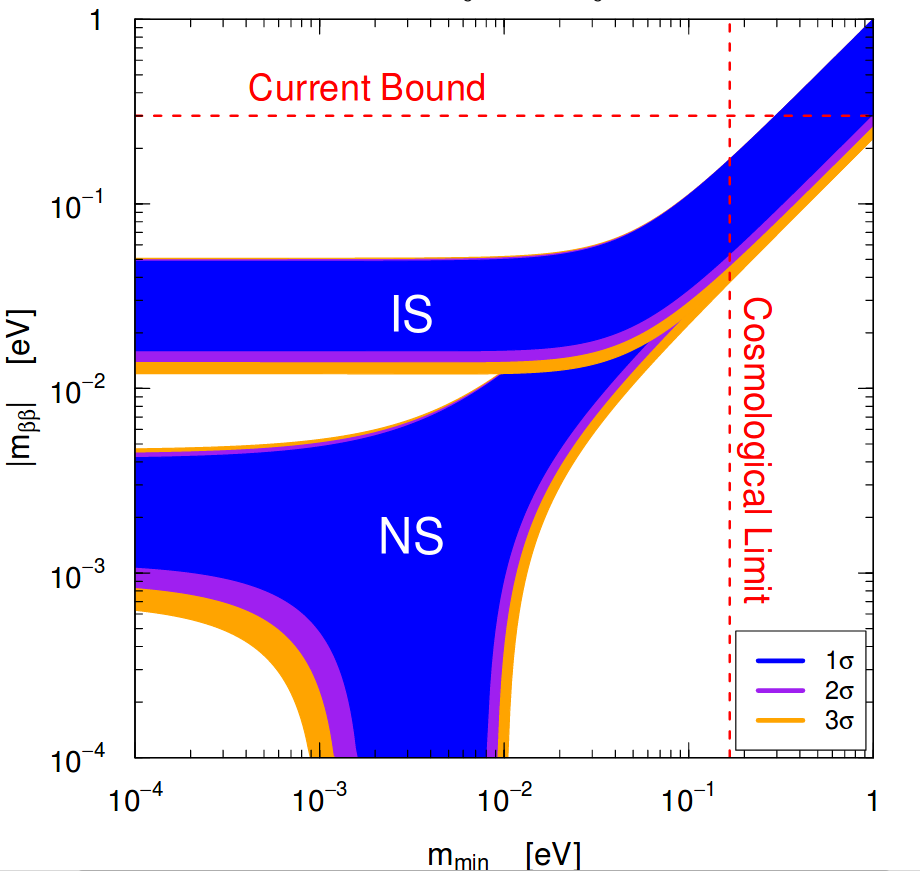
\includegraphics[width=\textwidth]{./Bilder/NeutrinoMassOrdering.png}
		\caption{Taken from \cite{bilenky_neutrinoless_2012}}
		\label{fig:MassOrder}
	\end{minipage}%
	\begin{minipage}{.5\textwidth}
		\centering
		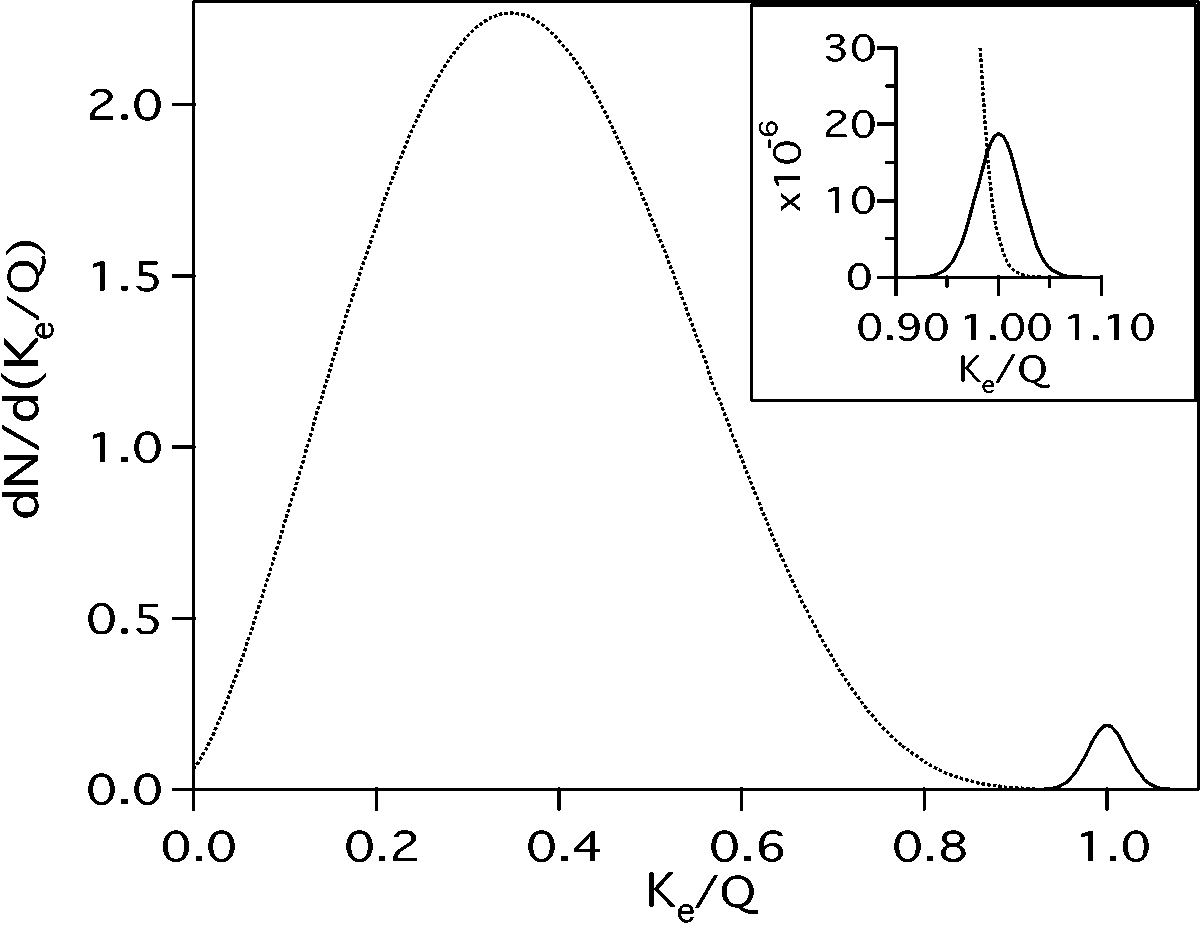
\includegraphics[width=\textwidth]{./Bilder/TheoretischesSpektrmdes0nubbDecay.png}
		\caption{Taken from \cite{elliott_double_2002}}
		\label{fig:TheoSpektrum}
	\end{minipage}
\end{figure}

But how exactly can you measured the \onbb\ decay?
Theoretically, the experimental signature of the \onbb\ decay is a sharp peak at the end of the regular \twonu\ decay (Q-value) from the effective spectrum of the two electrons (see figure \ref{fig:TheoSpektrum}).
As mentioned before there have only been a hand full of elements found to make \twonu\ decay and even less are actually useful for an experimental search of the \onbb\ decay.
A common experimental approach is to use a detector made of material enriched in a \onbb\-decaying isotope.
This has the advantage that the detection efficiency is maximized
\\

Since \onbb\ decay should have a very long half-life, a lot of background suppression must be used just to measure the resulting influence.
There are three kind of background sources that have to be considered.


The first radiation source originates from cosmic background radiation.
A great amount of muons shower down to the earth from the atmosphere and create background in the detectors.
Their influence can be suppressed by placing the experiment deep underground and applying a muon veto system.


Secondly, the background from natural radioactivity.
This is typically the dominant background source originating from radioactive isotopes which are naturally present in basically all materials.
Its influence can be suppressed by passively shielding the detectors and the selection of low radioactive components in the setup. 


Lastly the \twonu\ decay material itself creates background.
Its impact on the background can not be reduced by external measures or shielding.
However, by using a detector with high energy resolution or a decay material of high Q-value its influence can be suppressed.
\\

\nuc{Ge}{76} is an ideal material for the \onbb\ search due to it being a semiconductor.
It can therefor be also used as the detector material itself.
A disadvantage of \nuc{Ge}{76} is the low Q-value of $Q_{\beta\beta} = 2039\unit{keV}$, which is lower than \nuc {Tl}{208}'s and \nuc{Bi}{214}'s end point energy.
It is also hard to increase the target volume compared to e.g. \nuc{Xe}{136}.
But it can only be operated at cryogenic temperatures.
Otherwise it will not function properly.
Its advantage however is its ability to be made with great intrinsic radio-purity, its high energy resolution and its high detection efficiency.
These facts outweigh the disadvantages which is why it already has a history for being used as decay material and why it will be used in GERDA.
\\

%\nuc{Ge}{76} has a long history of use as decay material in \onbb\ experiments, most notably in the Heidelberg-Moscow(HdM) and the IGEX experiments.
%Both of these experiments are the predecessor experiments of GERDA.
%With detectors made of enriched germanium plus the background reducing precautions and active vetos described above they were able to set a similar limit of the half life of the \onbb\ to $\thalfzero(\nuc{Ge}{76}) > 1.9\times10^{25}\unit{yr}$ \cite{noauthor_phys._nodate}. 
%HdM experiment actually claimed to have measured the half life of about $\thalfzero(\nuc{Ge}{76}) = 1.19\times10^{25}\unit{yr}$ , but its legitimacy has been questioned by a part of the scientific community \cite{klapdor-kleingrothaus_search_2004}.
%\\

%This is where the  GERDA experiment comes in.
%Its first measuring phase (\PI) was planned to verify or falsify the results of the HdM experiment using the detectors used in the HdM and the IGEX experiment.
%\PI started in November 2011 and May 2013 with a total exposure  of  $21.6 \frac{\unit{kg}}{\unit{yr}}$ and no signal of a \onbb\ observed \cite{agostini_results_2013}.
%With its results and the results from HdM and IGEX a new lower limit for the half life was able to be set at $\thalfzero(\nuc{Ge}{76})>3.0\times10^{25}$  yr  (90$\%$ C.L.)
%The second phase (\PII) with 30 new custom-made enriched detectors together with the old detectors has started measuring in late 2015 and had its latest data published !!!! hier noch ob ich das NATURE paper quoten soll!!!!!.
%A more detailed description of the construction and functionality of the GERDA  \PII~ is the topic of the next section.

% also a bit about standard double beta decay
% differences between the standard and neutrinoless beta decay
 


\section{GERDA \PII}
\label{sec:GERDA}

% general Information, e.g. 
% sizes 
% Gran Sasso, 
% what other  neutrino less beta decay experiments are there,

\subsection{Experimental Setup}
\label{sec:ExSetup}
The GERDA experiment is located in the underground Laboratori Nazionali del Gran Sasso (LNGS) of INFN, Italy.
The laboratories are located approx. 1.4 km below ground, which corresponds to a water equivalent of 3.5km.
As already mentioned in the previous chapter the GERDA experiment uses \nuc{Ge}{76} as \onbb\ decay material as well as the detector material \cite{agostini_background_2017}.
\\

The detectors are operated bare in a liquid argon (LAr) tank of 64m$^3$ volume at an working temperature of about 90K.
This corresponds to a temperature light under the boiling point of LAr at normal pressure.
The argon being used was obtained from the atmosphere by air liquefaction and has been purified from radioactive isotopes by further distillation.
Its main purpose is to cool the germanium detectors down to their working temperatures and to shield against external radiation originating from the walls or the outside. 
Since \PII~ there are also photomultipliers positioned inside the LAr tank.
Due to the scintillation property of argon they measure a light signals whenever a charged particle travels through the LAr.
Because the \onbb\ decays are not likely to create any scintillation light the photomultiplier signals can be used as a rejection veto - the so called LAr veto.
\\

Situated around the LAr is a 590m$^3$ water tank.
Its main purpose is to shield the setup from outside radiation not only passively by absorption but also actively as a muon veto.
Situated in the water tank are 66 photomultipliers.
These detect any Cherenkov light created by high velocity charged particles passing through the water tank.
It can be expected that whenever an event is measured that the event was caused by an outside source and can therefor be rejected.
It therefor shares the same basic functionality with the LAr veto.   
Together, these two vetoes can identify  the majority of events.


Over the water tank is a clean room situated in which the detector strings can be assembled into the strings.  
The general setup can be seen in figure \ref{fig:GERDASetupPII}.
\\

Now to the detectors themselves.
GERDA \PII~ uses the seven coaxial detectors (COAX) that have already been used in the predecessor experiments HdM and the IGEX as well as 30 new broad energy germanium detectors (BEGe).
Both of these detector types are made of germanium that has been enriched from 7.8$\%$ of \nuc{Ge}{76} to about 87$\%$ \cite{agostini_background_2017}.
They also share the same basic functionality.
The major volume of both detectors are made of p doped germanium.
Both detectors have the majority of their surface covered by a 1-2mm thick n$^+$ doped electrode and only a small part with an p$^+$ electrode.
If an electron hole pair is created in the p doped area, the charged particles are separated and guided to the n$^+$ or the p$^+$ layer respectively by a strong electrostatic field (3 to 4 kV) between the electrodes.
It the pair is created in the n$^+$ layer the hole is most likely to recombine in the $n^+$ layer due to its low mobility and therefor creates no measurable signal.
The n$^+$ layer is therefor not not active and called a dead layer.
\\

The two detectors however differ in their design.
COAX detectors have a cavity coaxial to the cylindrical volume and are doped p$^+$ in the cavity's surface.
The BEGe detectors don't have a cavity.
They have a small p$^+$ doped surface at the bottom.
Sketches of their design can be seen in figure \ref{fig:DetcDes}.
The detector types also differ in their mass and therefor their expected exposure per detector and energy resolution.
The COAX detectors are generally heavier and therefor have a higher detector efficiency then the BEGe.
But their higher mass also results in a worse energy resolution \cite{agostini_production_2015}.
To compensate the fact that the BEGe detectors are generally lighter than the COAX a greater amount of them are being used.
\\

\begin{figure}[t!]
	\centering
	\begin{minipage}{.5\textwidth}
		\centering
		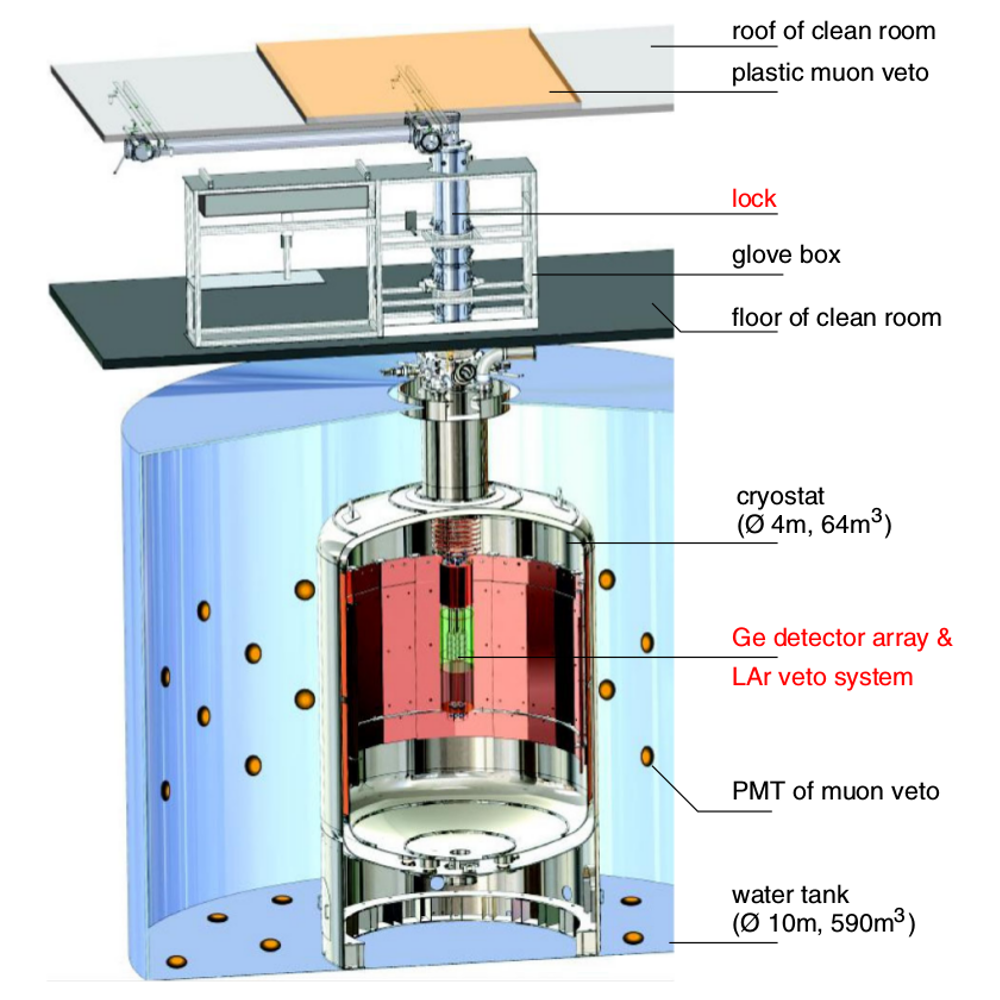
\includegraphics[height=60mm]{./Bilder/GERDAsetupPhaseII.png}
		\caption{Taken from \cite{collaboration_upgrade_2018}}
		\label{fig:GERDASetupPII}
	\end{minipage}%
	\begin{minipage}{.5\textwidth}
		\centering
		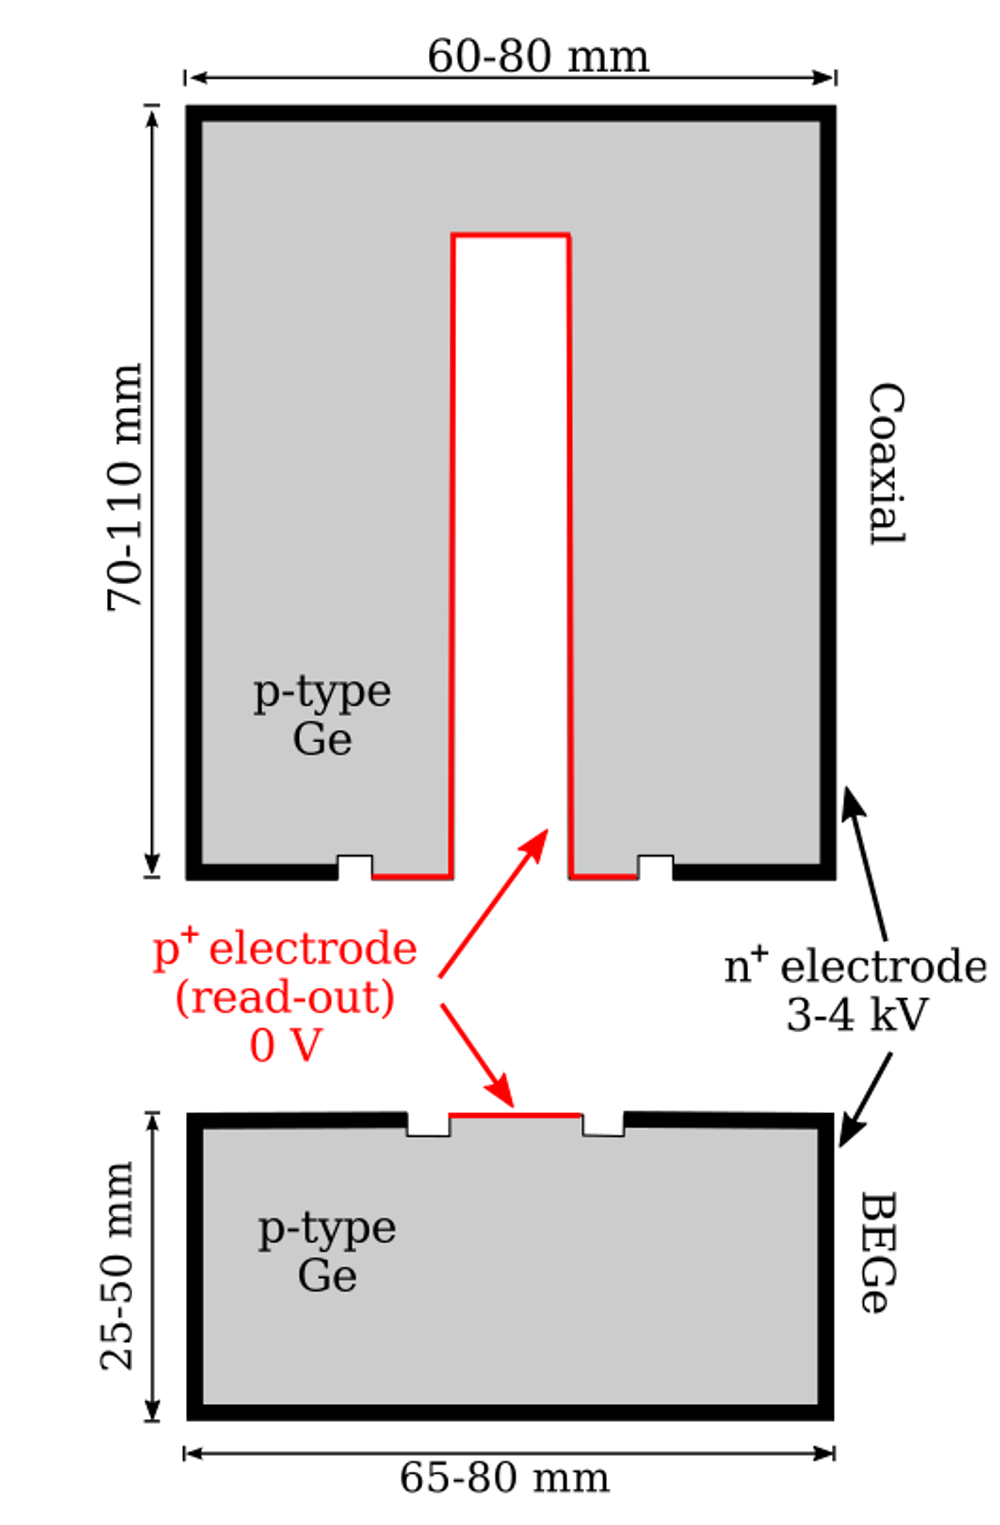
\includegraphics[height=60mm]{./Bilder/DetectorDesign.png}
		\caption{Taken from \cite{agostini_background_2014}}
		\label{fig:DetcDes}
	\end{minipage}
\end{figure}

The enriched detectors are assembled into 6 strings forming a hexagonal array together with a seventh string.
This seventh string consists of three extra coaxial detector made of natural isotopic \nuc{Ge}{76}.
However they are not used in GERDAs analysis.
The string setup can be seen in figure \ref{fig:strings} and \ref{fig:stringsabove}.
\\

All detectors are connected to custom made amplifiers also located in the liquid argon above the detectors.
The analog signal of every detector is then digitized at a sampling rate of 100MHz and in the case of an event stored for further analysis \cite{riboldi_cryogenic_2015}.
\\

\begin{figure}[t!]
	\centering
	\begin{subfigure}{.66\textwidth}
		\centering
		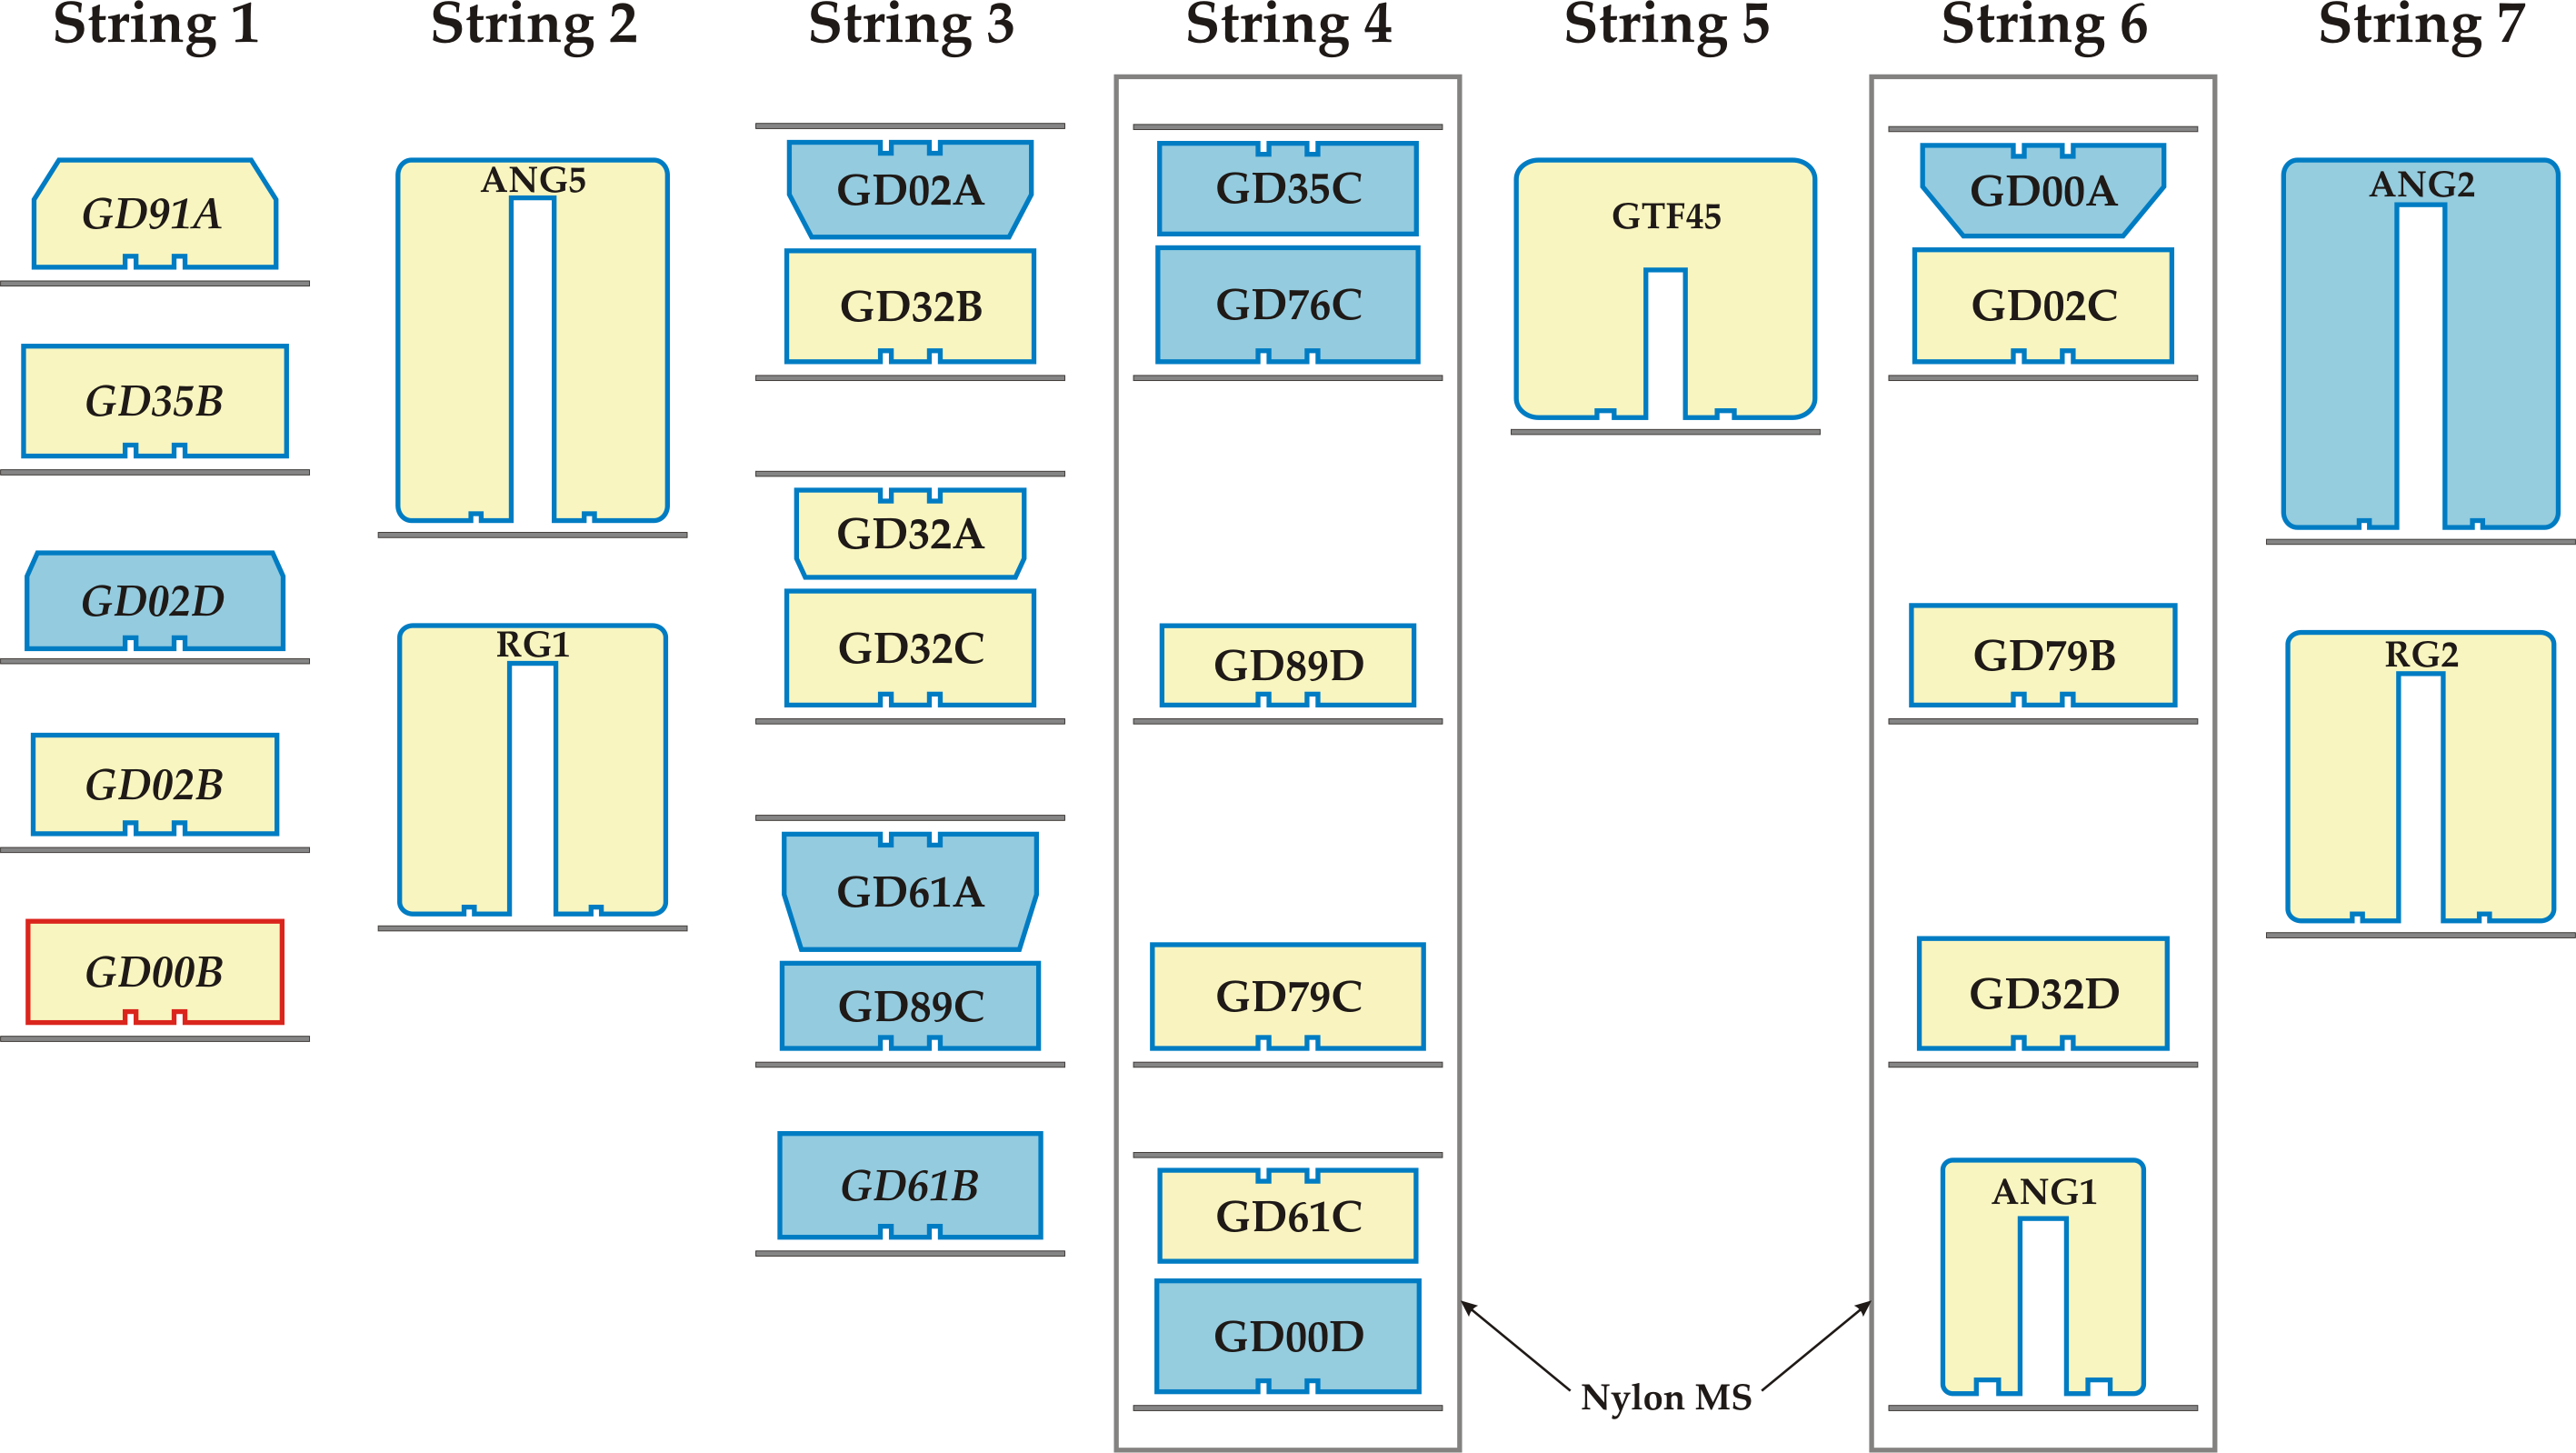
\includegraphics[width=.9\textwidth]{./Bilder/strings.png}
		\caption{}
		\label{fig:strings}
	\end{subfigure}%
	\begin{subfigure}{.30\textwidth}
		\centering
		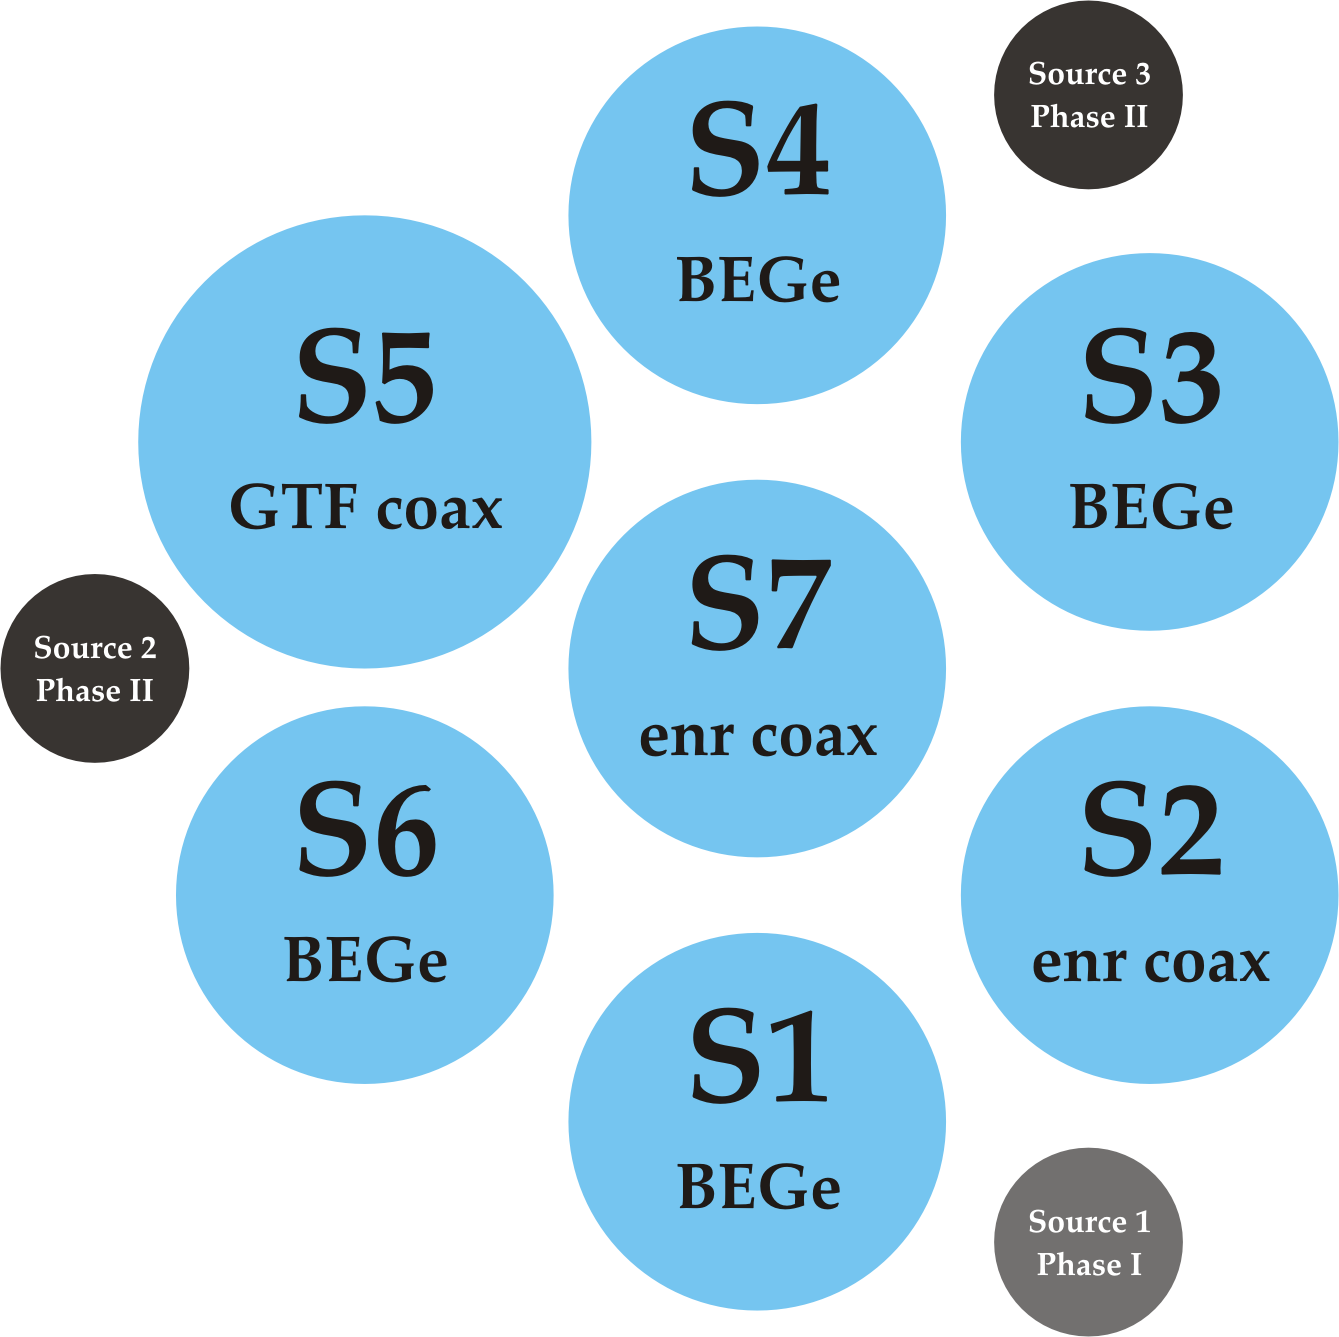
\includegraphics[width=.9\textwidth]{./Bilder/strings-top.png}
		\caption{}
		\label{fig:stringsabove}
	\end{subfigure}
\end{figure}
% well, just dump everything here
% also a bit about Tier1-4 storage of data 

The detectors are surrounded by a nylon cylinder to limit the amount of LAr volume around the detectors.
This is in place to passively suppresses the background created from \nuc{K}{42}.
Where the \nuc{K}{42} comes from and why its influence on the background can be repressed by this will be discussed later in section \ref{Discussion}.\\

\subsection{Liquid Argon as Coolant, Shielding and Scintillator} 
\label{sec:LArcoolant}

These nylon in the cylinder can be read out at their ends with silicon photomultipliers (SiPM) and are part of the LAr veto setup that will be the topic of this section.
\\

LAr has the property that scintillation light is produced when ionizing radiation interacts with an electron or nuclei within it \cite{olsen_improvements_nodate}.
Incoming radiation may excite or ionize the scintillation material along its way or collides with another particle which in return excites or ionizes other particles secondarily.
The excited atoms in a nobel liquids form dimer pairs (Ar$^*_2$).
These dimer pairs are metastable and recombine into two stable argon atoms by the release of a vacuum ultraviolet photon (VUV).
Depending on whether the argon atom was ionized or excited two different mechanisms are responsible for the relaxation.
But in the end each ionized or excited atom only produces one VUV photon and a direct correlation between the amount of energy deposited and the number of photons emitted can be found.
This correlation is called the scintillation yield and argon has a value of about $4\times10^4\frac{\unit{photons}}{\unit{MeV}}$ \cite{olsen_improvements_nodate}.
Nobel liquids also have the advantage that VUV light does not have enough energy to excite any ground state atom which is why the scintillation light can travel very long distances without being absorbed.
Compared to other nobel gases argon has the advantage of a very low price due to it being easily obtained by liquefaction of air from the atmosphere.
\\

\begin{figure}[t!]
	\centering
	\begin{minipage}{.30\textwidth}
		\centering
		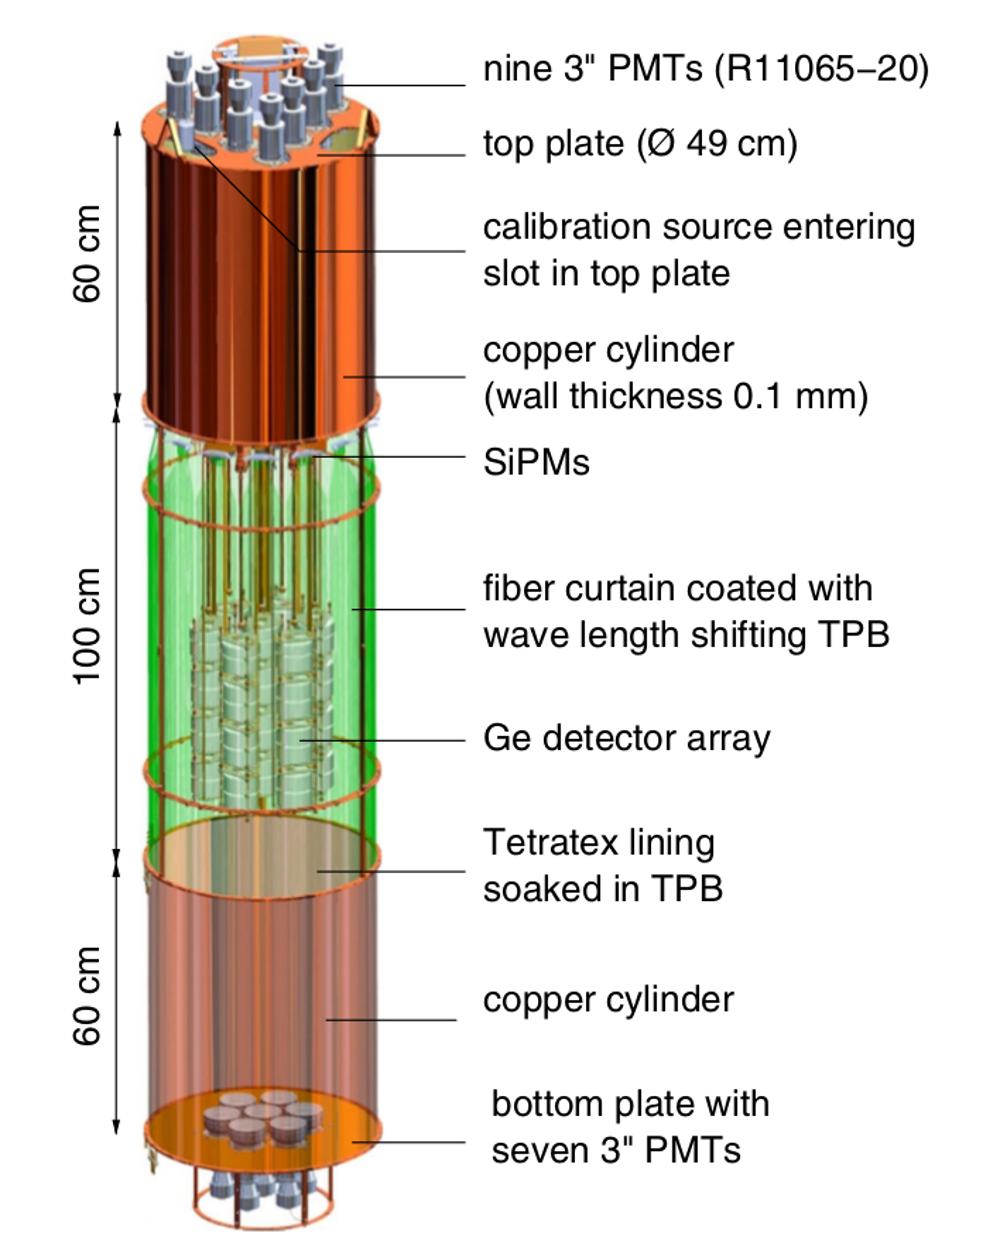
\includegraphics[width=\textwidth]{./Bilder/LArVetoSetup.png}
		\caption{Taken from \cite{collaboration_upgrade_2018}}
		\label{fig:LArVetoSetup}
	\end{minipage}%
	\begin{minipage}{.70\textwidth}
		\centering
		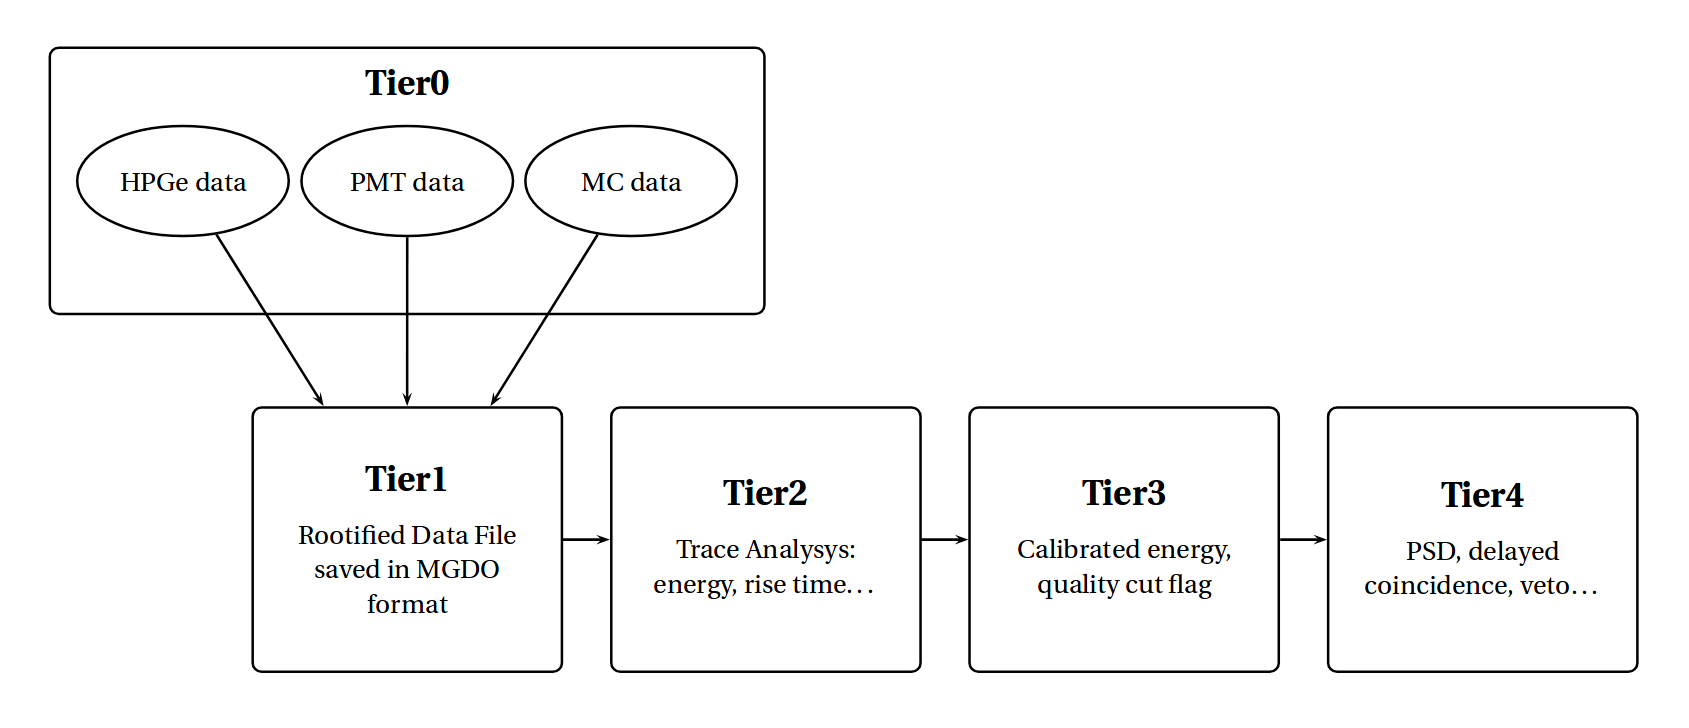
\includegraphics[width=\textwidth]{./Bilder/TierStructure.png}
		\caption{}
		\label{fig:TierStructure}
	\end{minipage}
\end{figure}

Background events often deposit energy in the argon while passing through it.
The scintillation light can therefor be used as a veto to filter out those events in which a coincidence between an event in the germanium detectors and a signal in a photomultiplier was measured.
A smaller cylindrical volume around the germanium detectors is therefor equipped with 16 photomultiplier tubes (PMT), situated at the bottom and at the top of this volume, as well as 90 SiPM that read out any light signal travailing through the nylon strings \cite{csathy_optical_2016}.
All signals measured in the photomultipliers are digitized and read-out in the case of an event in the germanium detectors.

Additionally, a wavelength shifter covers all nylon fibers and PMTs.
This shifter changes the wavelength of the LAr scintillation light from 128mn to 400nm.
At this wavelength the PMTs have their highest quantum efficiency as well as the nylon fibers their absorption maximum.
With this the overall detection is being increase.
The complete LAr veto setup can be seen in figure \ref{fig:LArVetoSetup}
\\

LAr is also a good coolant due to the characteristically low melting point of nobel gases.
At normal pressure argon has its boiling point at 87.29K and its melting point 83.8K.
The working temperature of GERDA is therefor chosen to be right under the boiling point temperature.
A low temperature is needed for the germanium detectors to function properly.
\\

Nobel liquids are also great as ultra radio-pure passive shielding.
This is because nobel elements rarely make any chemical bonds due to their fully filled electron shells.
It is therefor possible to filter the majority of impurity just by distillation.
Compared to Xenon it has a smaller interaction cross section due to its lower Z value but it is by far cheaper.
\\

\subsection{Data processing and analysis}
\label{sec:DataProc}

As already mentioned, in the case of an event the digitized signals of the gemanium detectors and the photomultipliers are stored for further offline analysis.
The software used for this purpose is GErda LAyouT for Input/Output (GELATIO).
It is a data analysis framework suitable for off-line digital signal processing and analysis of data recorded by germanium detectors.
It's advantages are its multiple level data organization and its modular digital signal processing.
These two points leave the analysis protocol incredibly flexible.
\\

The multi-tier structure used in GELATIO can be seen in figure \ref{fig:TierStructure}.
The raw data saved from the detectors and photomultipliers is stored in Tier0.
Theoretically, at this point in the process Monte Carlo created signals can be fed to the algorithm and processed just like actually measured events.
Tier1 has the same amount of information stored as Tier0 with the difference that it has been converted into a new encoding usable for the later analysis.
The higher-level-tiers contain different analysis results.
Tier2 stores the concrete output information obtained by applying the digital analysis onto the digitized signals like the uncalibrated energy and the raise time.
Tier3 stores information extracted from Tier2 like the energy of the event and some flags.
Tier4 also stores additional information like the pulse shape discrimination flag and further flags.
Additional information about the analysis process can be found in \cite{agostini_gelatio:_2011} and \cite{agostini_off-line_2011}.
\\

To ensure that the filter parameters of the analysis are set without bias, all events measured in a  50keV interval around the Q-value of the \twonu\ decay were only stored without any analysis applied at all.
Only after all parameters in the rejection process were finally defined all events from this interval analyzed will be analyzed. 
Such a procedure is called a blinding process and the revealing of the blinded events an unblinding. 
\\
% Mui, Mountain, Pulse shape disc.
% especially LAr-Veto 

\subsection{Recent Results}
\label{sec:ResultsofGERDA}

Only recently a new unblinding of all measured events at GERDA \PII\ so far  occured \cite{zsigmond_new_2018}.
In it only one event in the close proximity of the Q-value was measured.
By far too less to identify a peak at that value.
The conclusion was therefor that no evidence for a \onbb\ decay has been seen.
A new lower limit for \nuc{Ge}{76} was determined to be \thalfzero\ = $0.8\times10^{26}\unit{yr}$ (90$\%$ CL).
Currently GERDA receives an upgrade on the LAr veto and is planned to measured for untill 2020.
After that the successor experiment LEGEND in collaboration with the MAJORANA experiment it is planned to investigate the lower limit of \nuc{Ge}{76} half life further.

% what has happened so far

% short outline of approaches


\section{\Kr isotope}
\label{sec:Kry85}

\Kr has a mass number of A = 85 and an atomic number of 36.
Krypton is a noble gas 

\begin{figure}[t!]
	\centering
	\ifmakefigures%
	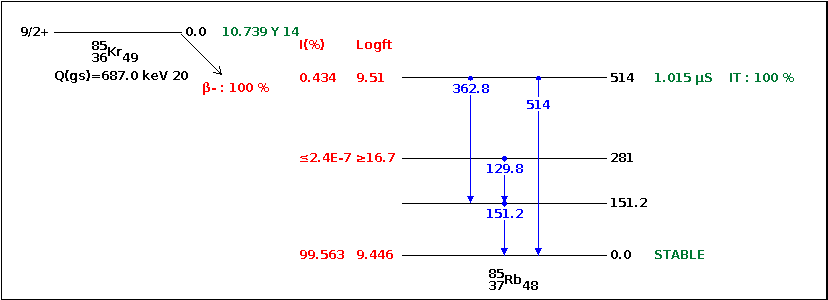
\includegraphics[width=.5\textwidth]{./Bilder/Kr85Decay.png}
	\fi%
	\label{fig:Decay}
	\caption{
		Taken from \cite{noauthor_decay_nodate}
	}
\end{figure}
% where does it come from?
% what properties does it have?
% why is it important to calculate its influence on GERDA

 
\chapter{Line Count Rate Analysis}
\label{sec:SAfrom514}


As stated in the introduction, the main goal of this theses is to approximate the specific activity of the isotope \Kr in the liquid argon coolant of the GERDA experiment. 
This value is of interest, as in other experiments this alien isotope in the liquid argon has produced a not negligible background. 
Two examples will be used in this thesis: the WARP and the Darkside experiment.
Both of these experiments have set their aim to detect WIMPs (Weakly Interacting Massive Particles) which are likely candidates for dark matter.
These WIMPs should in the case of their existence create tiny recoils in ordinary matter by elastic scattering.
Nobel gases are well suited as a target material, which is why many of today's dark matter experiments use them as target material.
Both WARP and Darkside have chosen liquid argon.
Due to the small expected interaction cross section of the WIMPs, the radioactive background sources have to be well known.
In both of these experiments a value for the specific activity of the residual \Kr has been determined.
In the Darkside experiment a specific activity of  \((2.86\pm0.18) \frac{\unit{mBq}}{\unit{l}}\)  \cite{agnes_results_2016} was measured whereas  \((160\pm130)\frac{\unit{Bq}}{\unit{l}}\) was measured for the WARP experiment \cite{benetti_measurement_2006}.
\Kr creates a non negligible background in the low energy statistics in both experiments but of very different proportion. 
It is therefor of interest to determine the specific activity in the GERDA experiment if one wants to use the low energy interval for other kinds of research.
For example for a further investigation of \nuc{Ar}{39} with a similar Q-value as \Kr or the search for dark matter in the keV-scale.
%This corresponds to a concentration of about \((2.32\pm0.14)\times10^{-18}\frac{\unit{mol}}{\unit{l}}\) for the Darkside and  \((1.30\pm1.05)\times10^{-16}\frac{\unit{mol}}{\unit{l}}\) for the WARP experiment.
\\

As already mentioned in the introduction, two different approaches are used in this theses to calculate the concentration of \Kr. 
The first and more precise method is the line count rate analysis of the \Kr decay into an excited state of \nuc{Rb}{85m}. 
It is also the topic of this chapter.
The second method discussed in the following chapter uses the reduction in count rate over time. 
This method is less likely to create precise results due to it relying on the assumption that only \Kr's activity has a notable change over time.
It is therefor only planned as a crosscheck for the result of the first method.
\\

Now to how the line count rate analysis can determine the specific activity of an radioactive isotope.
As discussed in section \ref{sec:Kry85}, \Kr has a small probability of 0.43\% to decay into an excited state of \nuc{Rb}{85m}. 
This state has a raised energy level of 514keV compared to its ground state and a half-life of 1.015\(\unit{\mu s}\). 
Theoretically it should be possible to measure a peak in the spectrum around the 514keV energy mark caused by the photons emitted from this relaxation.
Around this peak a Gaussian peak fit can then be apply to determine the number $N_{peak}$ of events measured in this area. 
\\

It is also necessary to calculate an efficiency of the detectors to measure a photons with an energy of 514keV.
This detector efficiency has to be determined using a Monte Carlo simulation.
This simulation creates a huge amount of 514 keV photons $N_{sim}$  in a constant volume $V_{sim}$ and counts the measured events in the detector $\Delta N$. 
The detector efficiency can then be calculated by dividing the measured events by the total number of simulated decays ($\epsilon = \frac{\Delta N}{N_{sim}}$).
This value can then be used in a conversation factor $\frac{1}{\epsilon V_{sim}}$ to determine the amount of decays per liter necessary to create the measured peak.
\\

The final value needed to calculate the specific activity is the measuring time $\bar{t}$.
Not every detector was measuring over the course of Phase II.
This is why a mean measuring time of all detectors has to be calculated.
With these three values plus the probability of the decay into the excited \nuc{Rb}{85m}, a mean specific activity $\bar{a}$ can be determined by inserting the values into this function:

\begin{equation*}
    \bar{a} = \frac{N_{peak}}{p}\times\frac{1}{\epsilon V_{sim}}\times\frac{1}{\bar{t}}
\end{equation*}\\

The line count rate analysis is expected to generate a relatively precise estimation of the specific activity.
This is because only photons from the \nuc{Rb}{85m} relaxation can create this signal.
\\

However, a problem of this method lies with the proximity of the \Kr to the 511keV peak of the positron electron annihilation. 
Its signal is expected to partially dominate over the \Kr in the spectrum and does not allow for a direct measurement of the 514keV peak. 
This is not necessarily a great setback because we can just adapt our fit function to a double Gaussian peak function.
It is of interest however whether it is possible to completely suppers the annihilation peak without changing the 514keV photon line count.
For this one could consider using the LAr veto.
Due to the low mean energy of the escaping electron (47.65keV) of this decay, it is very unlikely that it creats any scintillating light. 
On the other hand one can expect the light of the positron electron annihilation to create a great signal in the photomultipliers.
Therefor it should be possible with the LAr veto to single out the 514keV photon events from the annihilation events.
If possible this could be a second approach to determine the amplitude of the peak without adjusting the fit function.

The rest of the chapter will cover the concrete implementation of the individual steps in their own sections.
\\
\section{Preparing the spectrum}

As it was stated above, to determine the amount of measured 514keV photons a fit has to be applied onto the 514keV peak. 
But before the measured spectrum can be used for further analysis some filters have to be applied first.
These filters should reject any event of which we can say that they can not be caused by a \Kr decay.
Two very appropriate filters for this purpose are the Muon Veto and the detector anti-coincidence veto.
How exactly these two filters are used in this analysis will now be discussed.
\\

As it was elaborated in section \ref{sec:DataProc} all GERDA data is stored in a multi-tier data structure. 
In this thesis only the data from tier 3 or tier 4 will be used.
On these two levels a lot of analysis has already been done on the original data. 
As part of the Muon veto, each event in tier 3 and 4 was given a flagwhether or not aat the same time asignal in one of the photomultiplier in the water tank was detected. 
Due to the low kinetic energy of the beta electron of the specific \Kr decay in a non background event the Muon Veto flag should not be trigged.
It can therefor be used to lower the amount of background events in the investigated energy area.
\\

For a photon from the relaxation of \nuc{Rb}{85m} to create the 514keV peak it has to deposit all of its energy in one and only one detector. 
This means that any event in which two different germanium detectors have measured a non negligible energy depositions is most likely not caused by a \Kr decay.
This kind of rejection protocol is called a detector anti-coincidence veto.
Whether an event has more than one detector measure a signal can be determined by the multiplicity counter of each event stored in tier 3 or 4.
Using only those events in which this counter is set to one, even more background of none \Kr decays can be suppressed.
\\

After applying the first few filters on the spectrum one has to also make a distinction in which of the detector an event was measured.
As it was elaborated in section \ref{sec:ExSetup}, two different types of detectors were used in GERAD \PII\ - the BEGes  and the COAX. 
Due to their differences in design and weigh the two types have a different energy resolution and detector efficiencies. 
The BEGes are generally smaller and therefor have a higher energy resolution compared to the rather big COAX detectors.
For example, at an energy of 514keV the BEGes have a resolution of about 2.267keV while the COAX detectors are about 0.5keV higher at 2.72keV (see appendix \ref{sec:} ) \cite{agostini_background_2017}. 
But due to the BEGes being smaller they also have a lower detection efficiency.
It is therefor necessary to evaluate their measured data separately.
\\

After the adjusting the spectra to a lower background level, one can now determine more precisely the number of measured events in the 514keV peaks of the corresponding detectors (see figure \ref{fig:NoFilterBEGes} for the BEGes and \ref{fig:NoFilterCOAX} for the spectra of the COAX detectors). 
In these two spectra one can see two peaks - one at 511keV that corresponds to the positron electron annihilation events and one at 514keV that corresponds to the photons from the relaxation of \nuc{Rb}{85m}.
From this we can already claim that there must be a non negligible amount of \Kr in the liquid argon.
Otherwise no peak should have been able to be measured. 
The difference in resolution as discussed above can be seen in the fact that in the BEGe diagram the two peaks have a smaller full width at half maximum (FWHM).
Compared to the COAX detectors their peaks can easily be distinguished.  
\\

\begin{figure}[t!]
\centering
\begin{subfigure}{.5\textwidth}
  \centering
	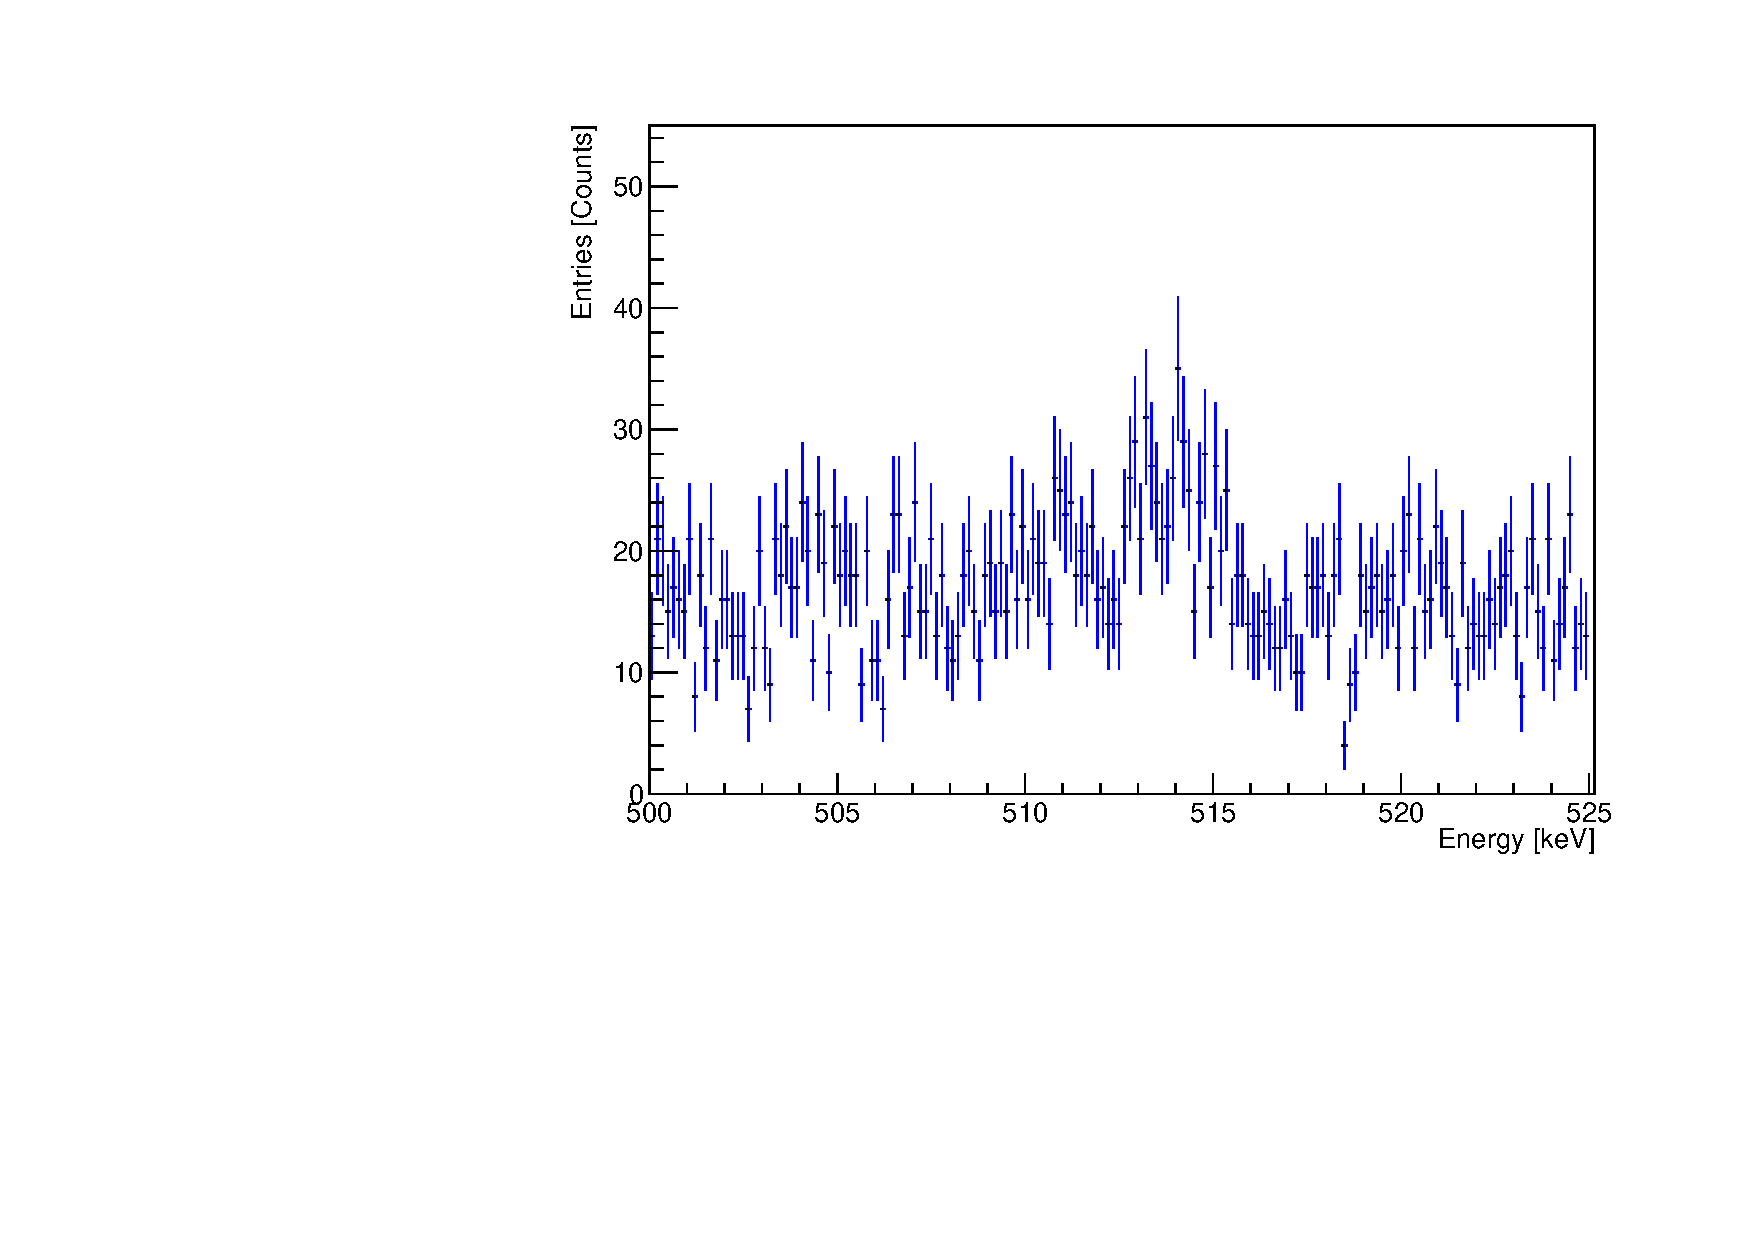
\includegraphics[width=75mm]{./Bilder/500525NoFilterBEGes.pdf}
  \label{fig:NoFilterBEGes}
  \caption{BEGes}
\end{subfigure}%
\begin{subfigure}{.5\textwidth}
  \centering
	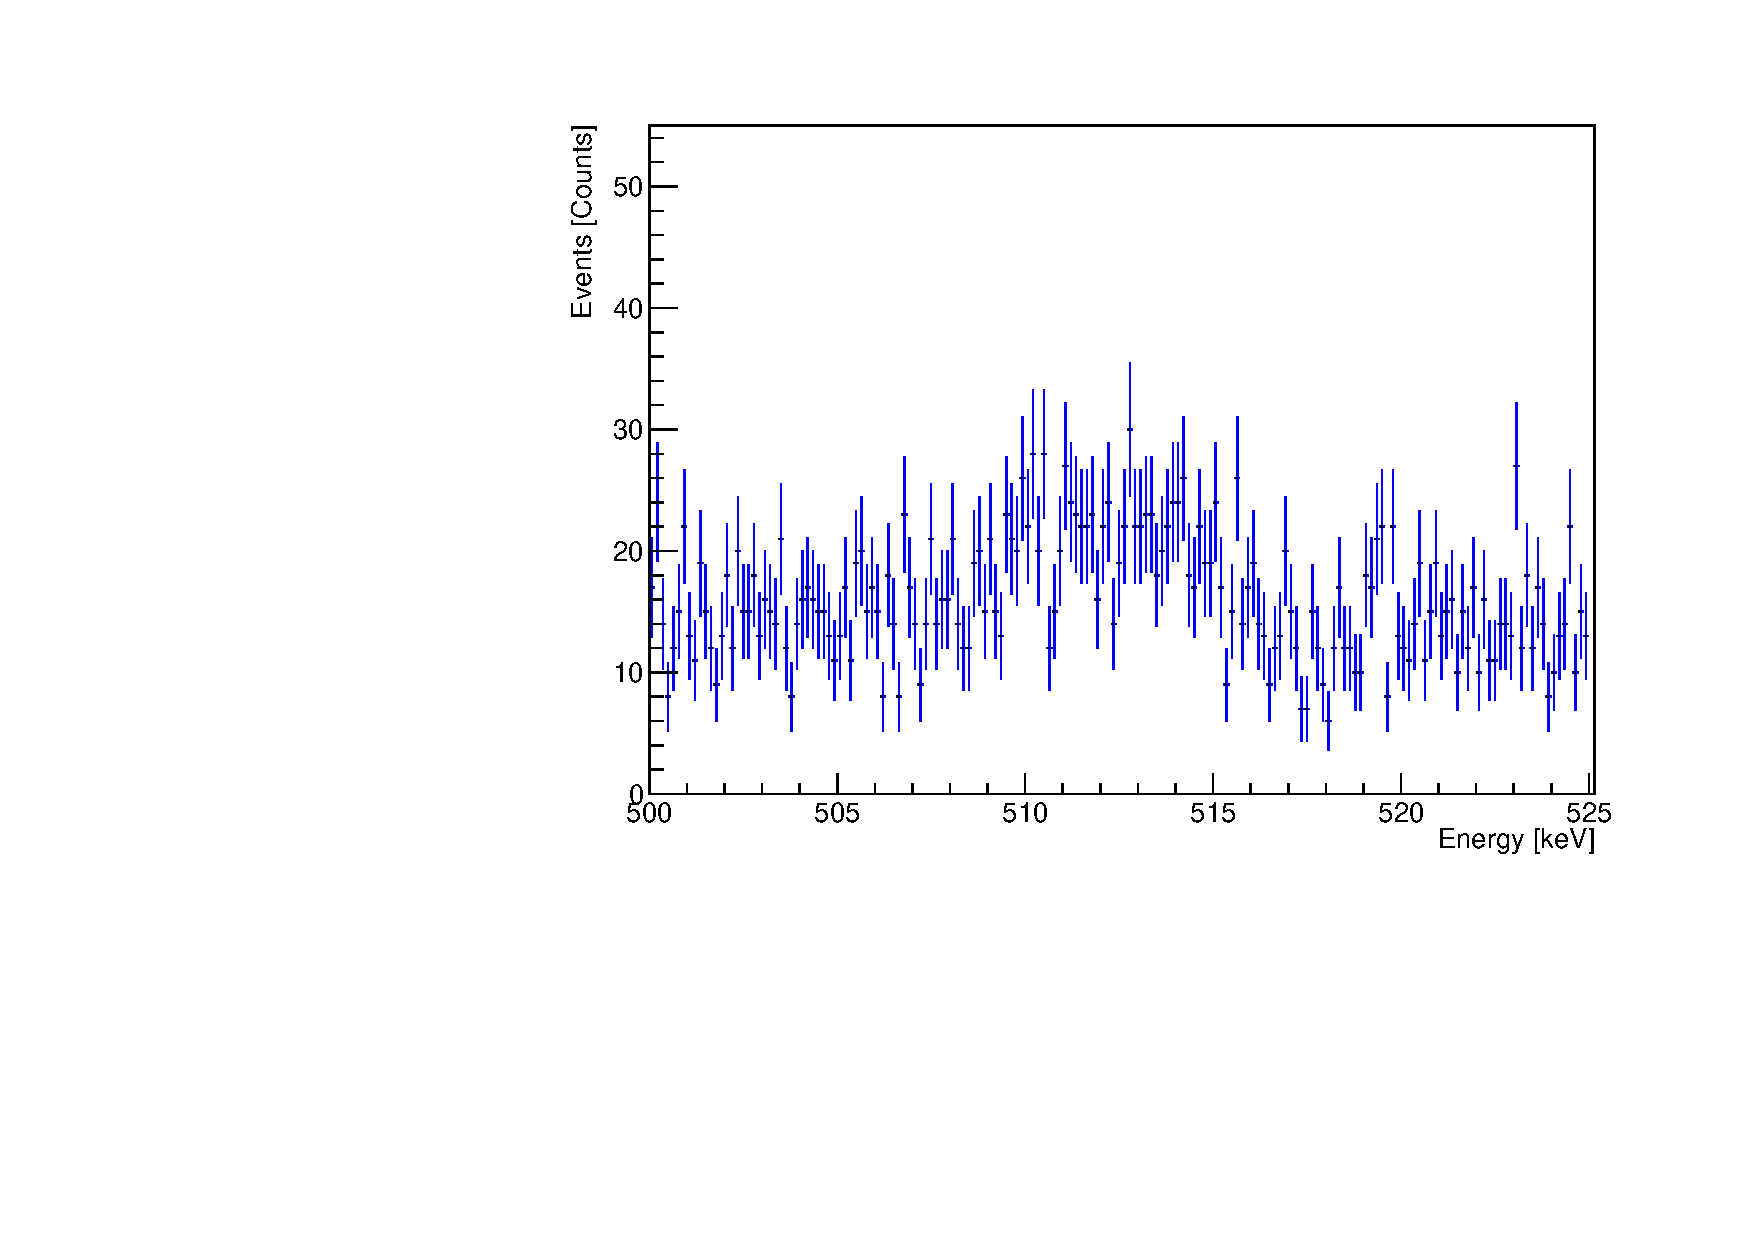
\includegraphics[width=75mm]{./Bilder/500525NoFilterCOAX.pdf}
  \caption{COAX}
  \label{fig:NoFilterCOAX}
\end{subfigure}
    \\
	\vspace{0.5cm}
	\caption{All events measured by the respective detectors in the range of 500keV to 525keV.}
\end{figure}

Now that the two spectra of the corresponding detectors have been determined, two possible ways determining the number of events in the 514keV peak have to be considered.
One way uses the spectra as they are and only adjusts the fit function so that it also takes the second peak into account.

Another possible approach suppress the annihilation peak using an almost ideal filter and fit the resulting one peak spectrum with the original fit function.
As mentioned above the LAr Veto should be a good candidate for such a filter.

In this thesis both approaches will be applied separately and later their results compared.
Hopefully both will end up delivering the same result as no \Kr caused event should make a notable light signal.
But this probability is not zero which is why some events of the 514keV peak might also trigger the veto.
This would result in a smaller peak amplitude and with it a lower specific activity than the actual value. 
Whether or not a rejection process using the LAr veto would be useful in this analysis or not is the topic of the following section.
\\

\section{Annihilation Peak Suppression}
\label{sec:APS}

Like the Muon veto, Tier4 assigns a flag to each event called "isLArVetoed".
This flag is always triggered when an event in the Germanium detectors coincides with a scintillation signal of at least 0.5phe in one of the photomultipliers in the LAr \cite{agostini_background_2017}.
If one plots all events in which this flag has not been set into a histogram, one results spectra seen in figure \ref{fig:LArBEGes} for the BEGes and figure \ref{fig:LArCOAX} for the COAX detectors.
One can see that the positron electron annihilation peak can not be identified any longer while the 514keV.
\\

\begin{figure}[t!]
\centering
\begin{subfigure}{0.5\textwidth}
	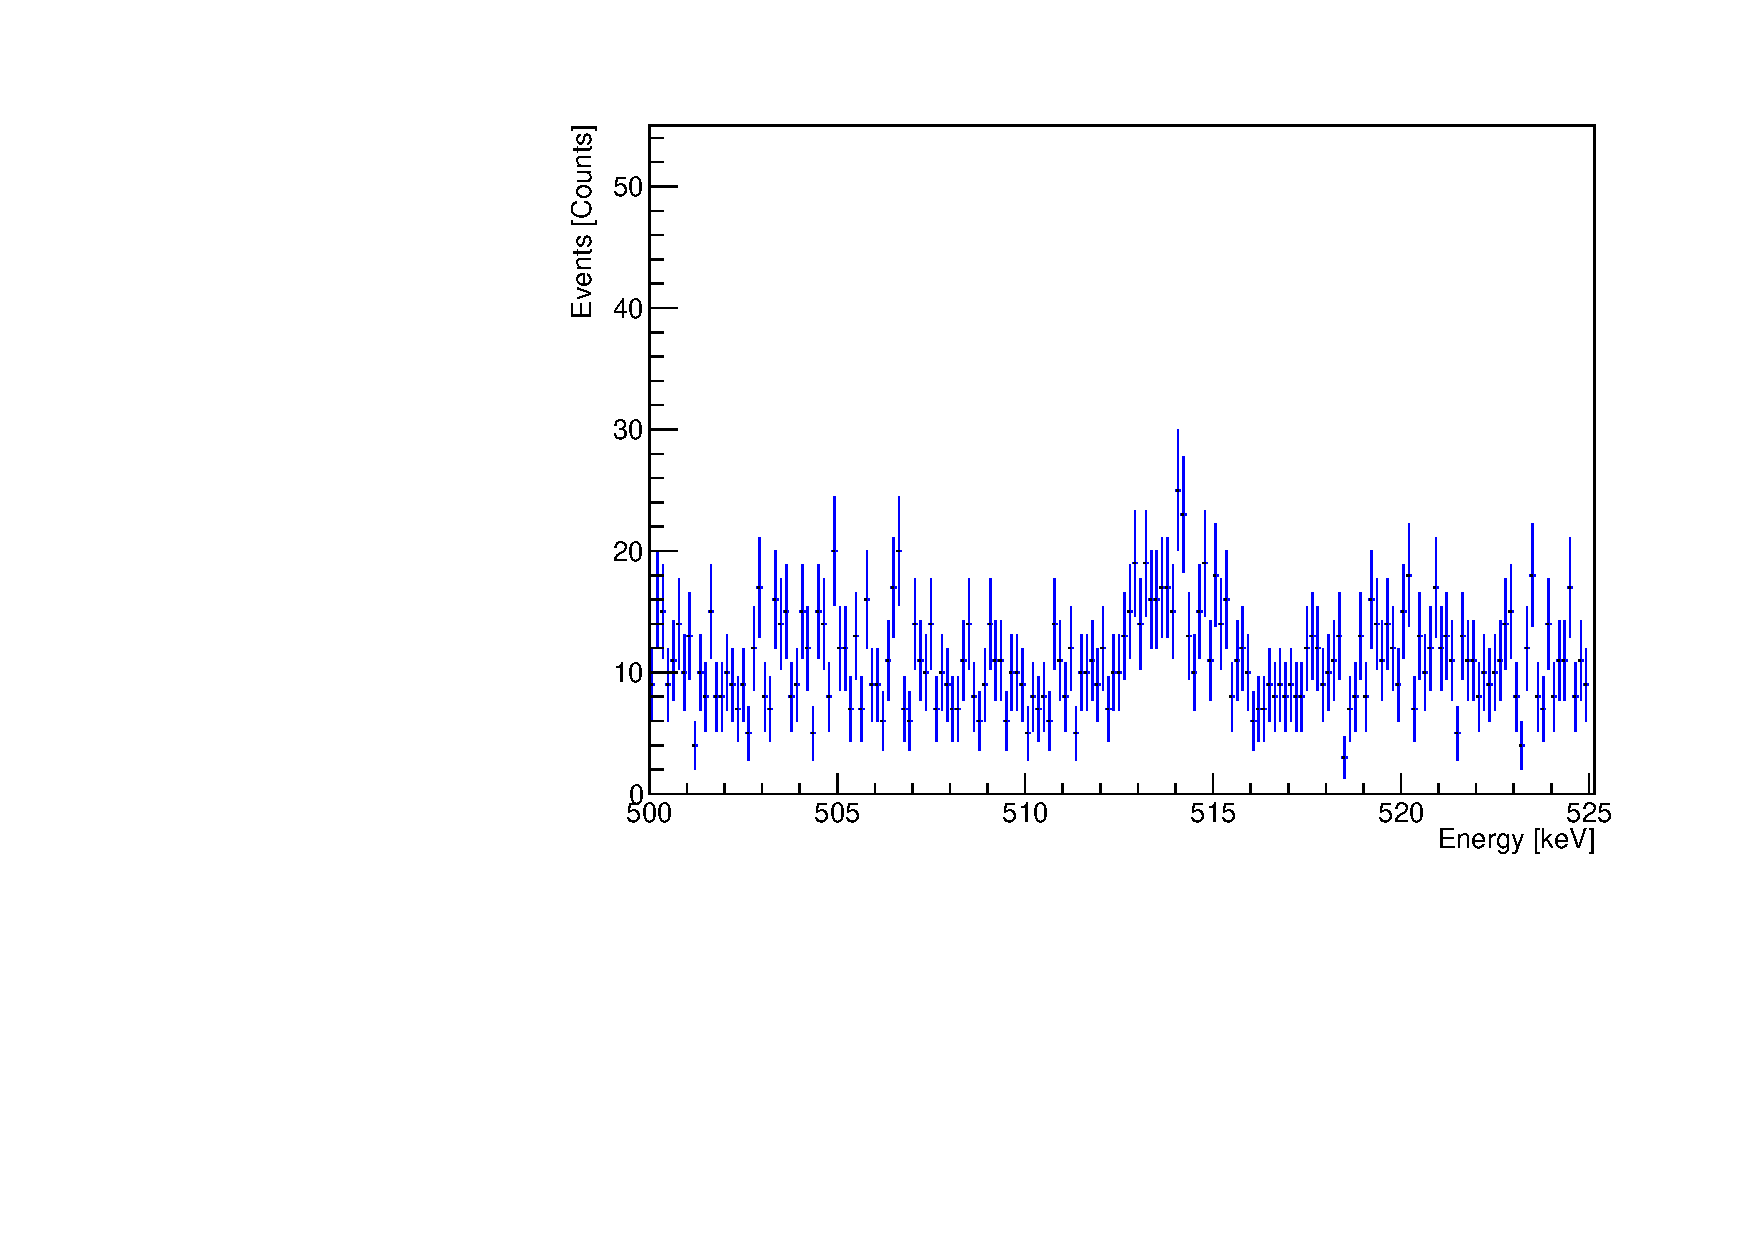
\includegraphics[width=75mm]{./Bilder/500525LArVetoBEGes.pdf}
    \caption{BEGes}
  \label{fig:LArBEGes}
\end{subfigure}%
\begin{subfigure}{0.5\textwidth}
	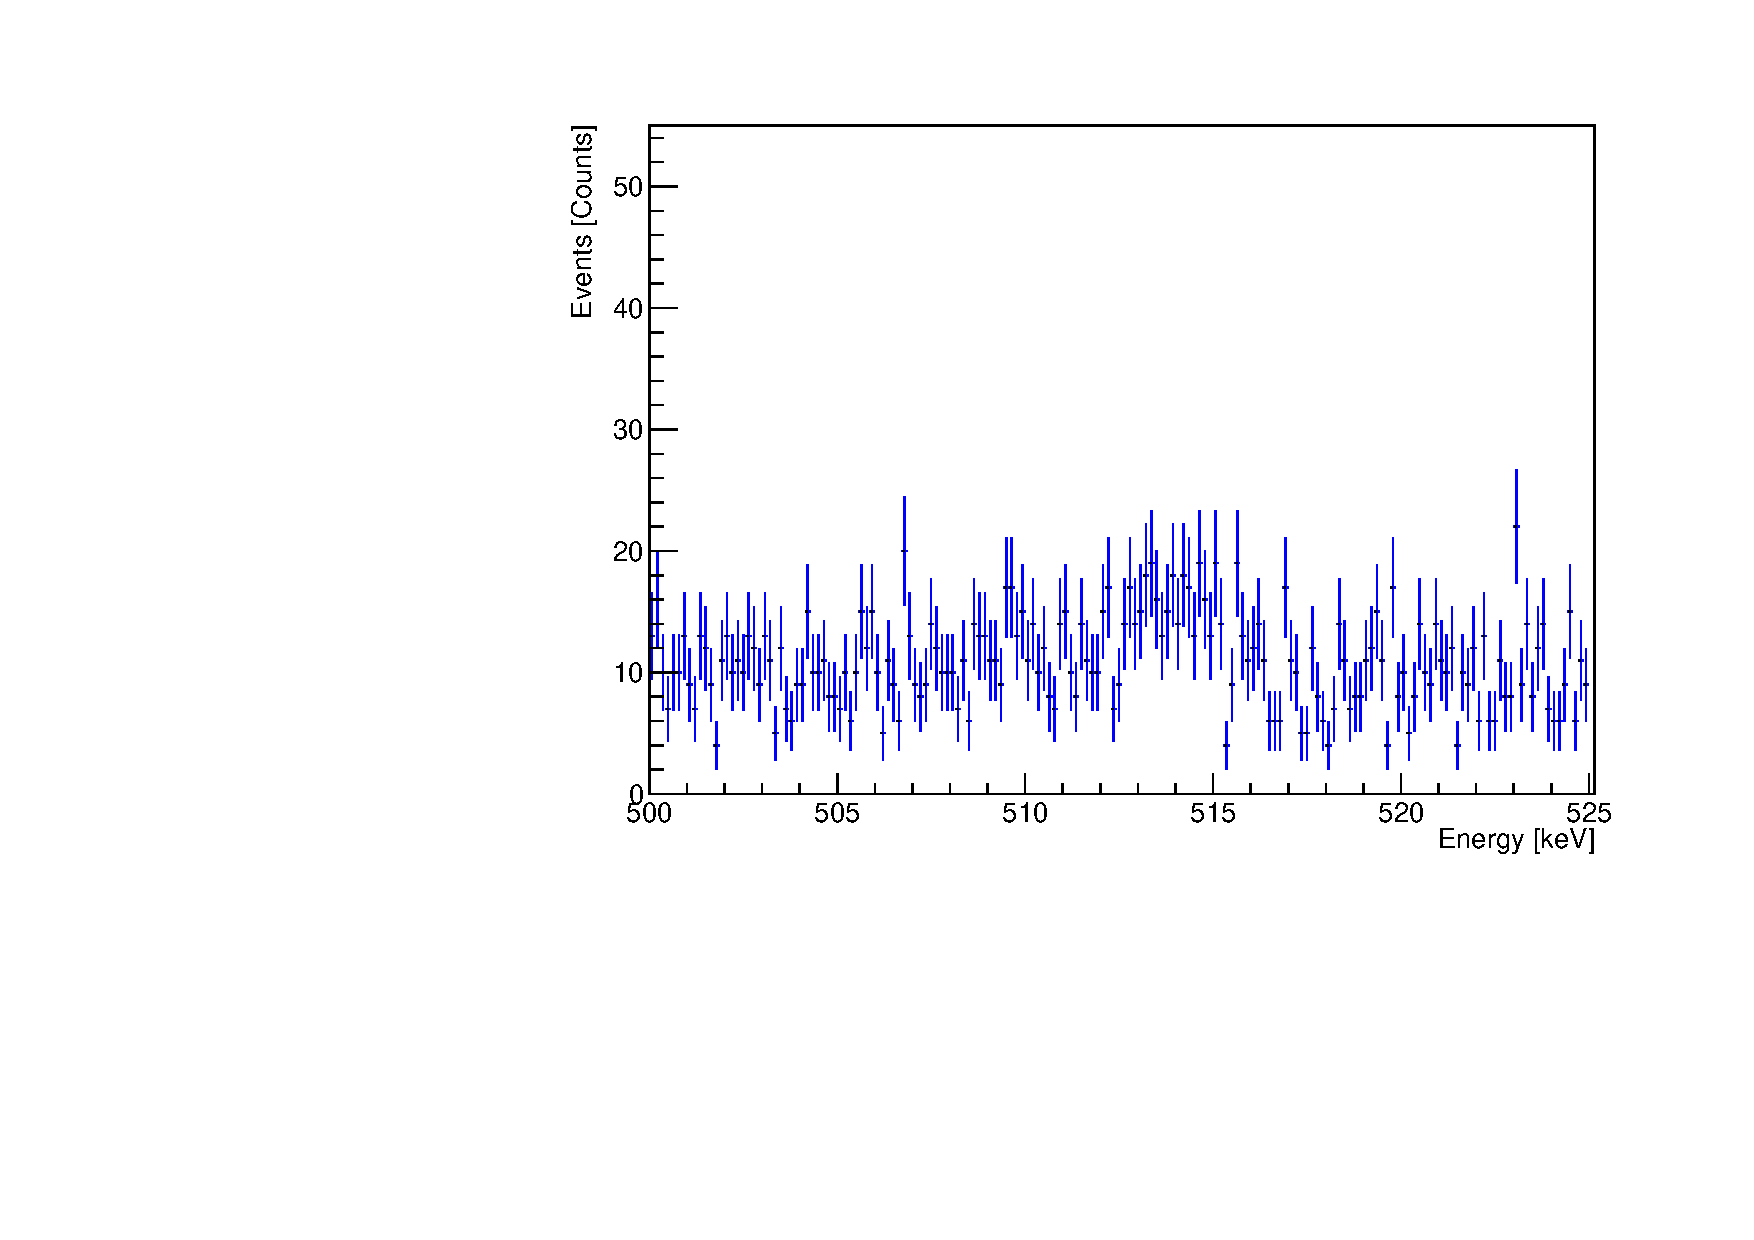
\includegraphics[width=75mm]{./Bilder/500525LArVetoCOAX.pdf}
  \caption{COAX}
  \label{fig:LArCOAX}
\end{subfigure}
    \\
	\vspace{0.5cm}
    \caption{All events measured by the respective detectors with the LAr filter applied in the range of 500keV to 525keV.}
\end{figure}

\begin{figure}[t!]
	\centering
	\begin{subfigure}{.5\textwidth}
		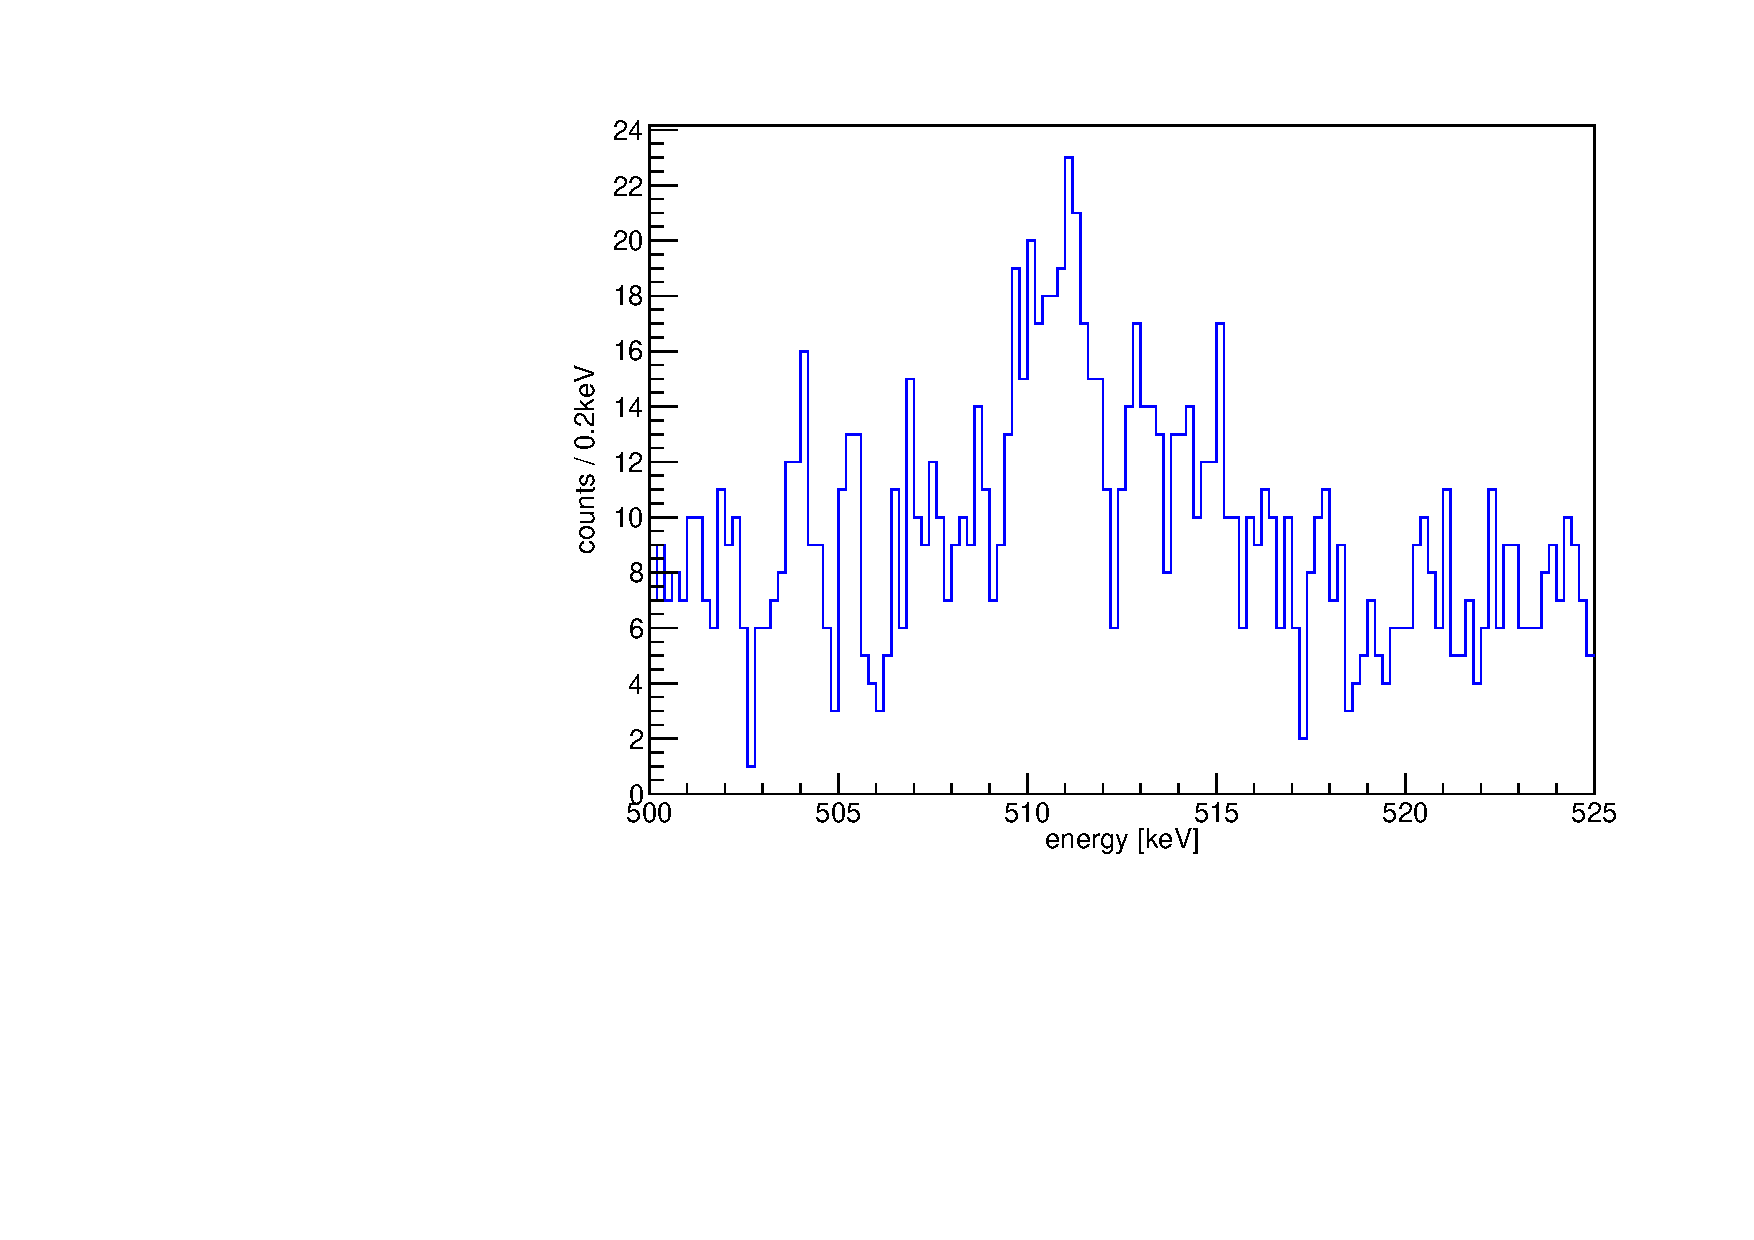
\includegraphics[width=75mm]{./Bilder/AntiLArBEGe.pdf}
		\caption{BEGes}
		\label{fig:AntiLArBEGes}
	\end{subfigure}%
	\begin{subfigure}{.5\textwidth}
		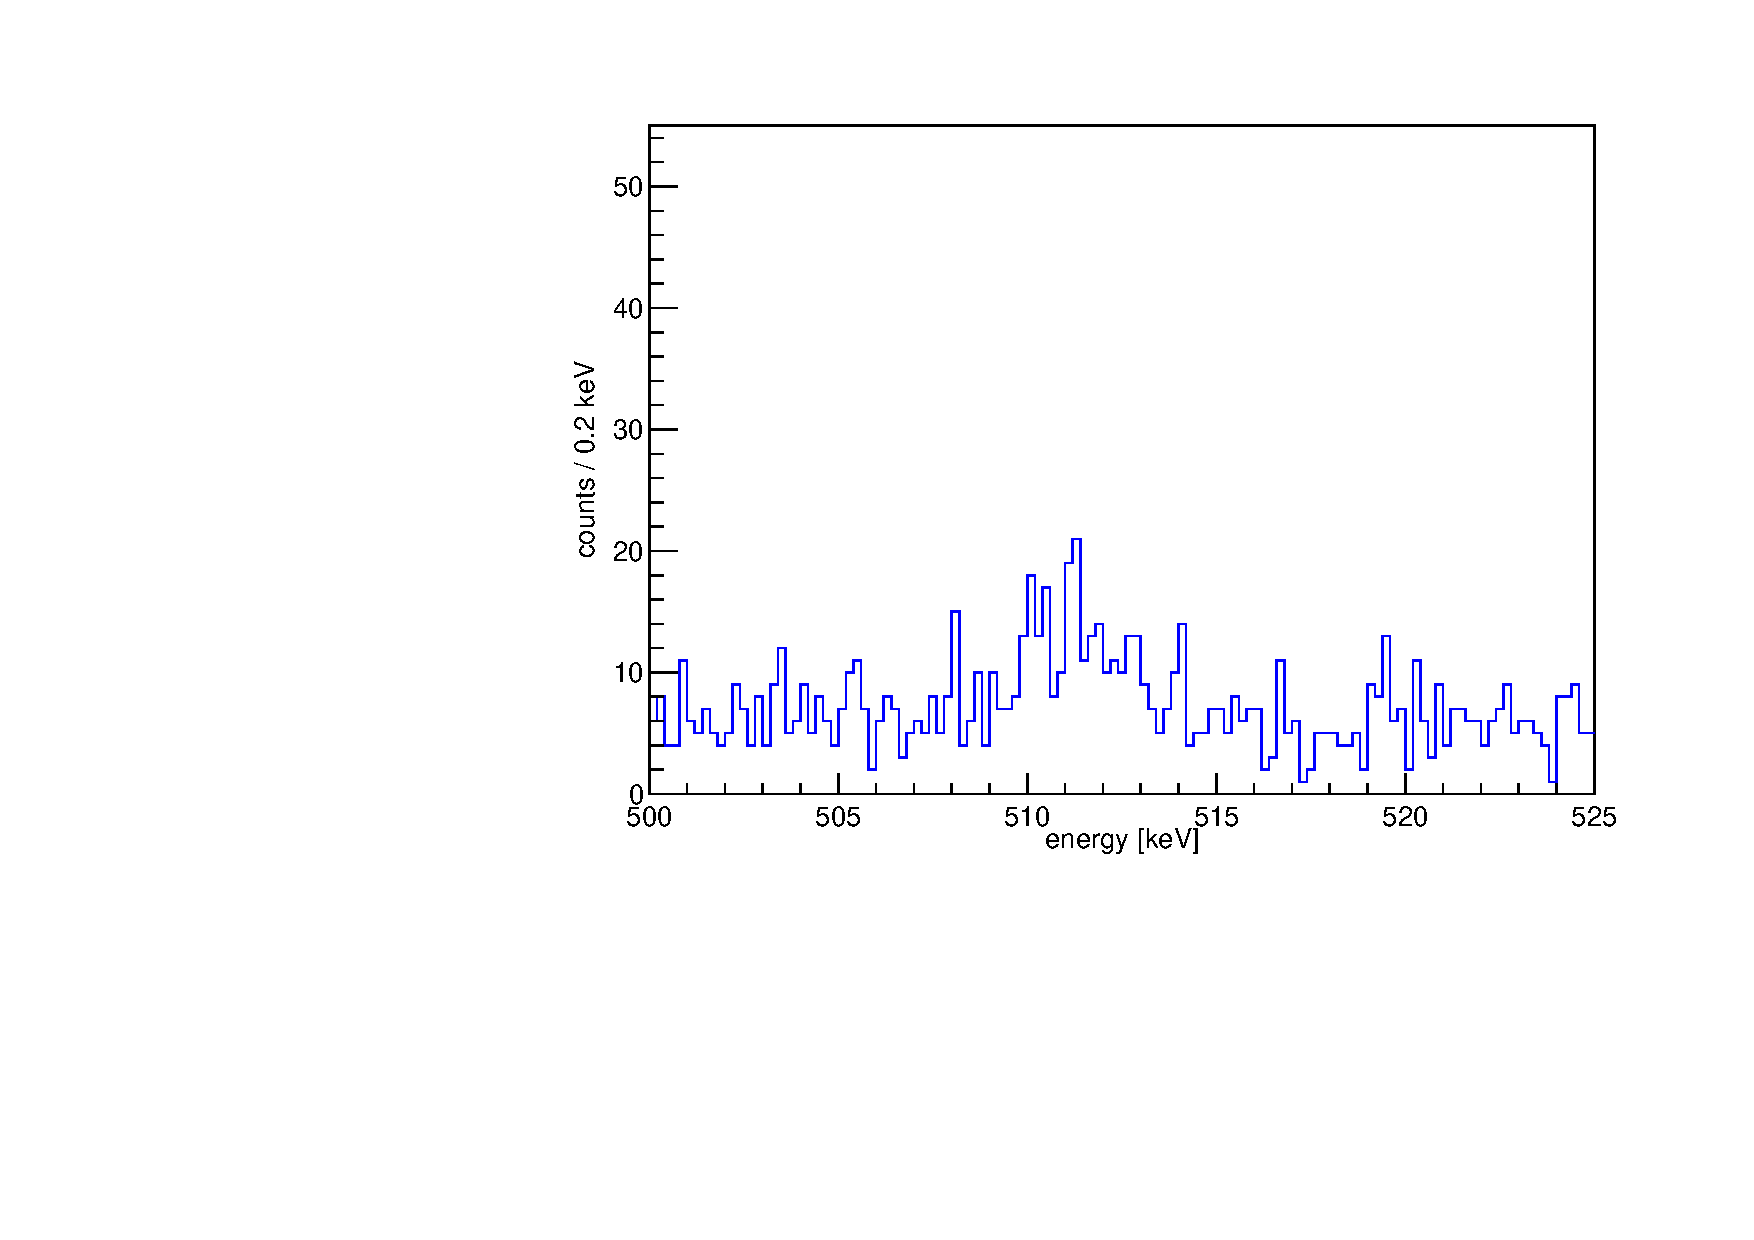
\includegraphics[width=75mm]{./Bilder/AntiLArCOAX.pdf}
		\caption{COAX}
		\label{fig:AntiLArCOAX}
	\end{subfigure}
	\\
	\vspace{0.5cm}
	\caption{All events measured by the respective detectors with the LAr filter applied in the range of 500keV to 525keV.}
\end{figure}

In order to visualize it better which events have been rejected, you can also take all those events that triggered the LAr veto (figures \ref{fig:AntiLArBEGes} and \ref{fig:AntiLArCOAX}).
From those you can see that the majority of the filtered events had an energy around the 511keV mark.
But one can also see from these figure that a small number of 514keV peak events have been rejected.
This means that some of the events caused by \Kr decays must also have coincided with scintillation light.
\\

Because the line count would in this case be smaller than in the unfiltered case it is of interest to investigate whether some of the \Kr decay caused events might be possible to recover.
The absolute number of events filtered out by the LAr veto in the energy range of 509 to 519 keV is 1728.
This number is too big to look at every individual case manually.
\\

Luckily, the excited \nuc{Rb}{85m} state has a half life of 1.015 \(\unit{\mu s}\).
This means that one should be able to measure pre-coincedence events of the beta creating scintillation light before the germanium detector event.
This way one can hopefully identify the majority of events created by \Kr decays over the rest of the filtered signals.
For this purpose, the events used for the investigation must be limited to those that have a negative time difference between the germanium events and the photomultiplier signal.
The time difference for each individual liquid argon events is already analyzed and stored in the vector $"$triggerLAr$"$ of the Tier3 data set.
This vector has the same number of dimensions as photomultipliers and each entry is indexed with the corresponding input channel of one.
The entries of this vector are again vectors that store the time difference for each signal that triggered the LAr veto in the corresponding channel.
Since only the earliest trigger event of the photomultiplier is of interest for the analysis,  for reasons of simplicity only the first entry of this internal vector will be used as they are ordered in ascending order.
From this point, only events where at least one photomultiplier has measured a negative time difference are used for the recovery analysis.
\\

In addition, as already mentioned earlier, the energy of the released beta electron is very low.
This means that one can expect from a \Kr decay into an excited state of \nuc{Rb}{85m} that only a small number of photomultipliers should measure a signal.
This is because the effective scintillation yield of the GERDA setup is about 60 phe/MeV.
With a mean energy of 47.65keV one can expect that to measure 1 to 4 photons per decay.
Therefore, only events with a maximum of four different triggered photomultipliers are used in the further analysis.
This amount of coincedently triggered photomultiplier leaves still a lot of events.
But due to the fact that later in the analysis a manually investigation into the individually measured events will be performed the filter can be a little coarser here.
\\

\begin{figure}[t!]
	\centering
	\ifmakefigures%
	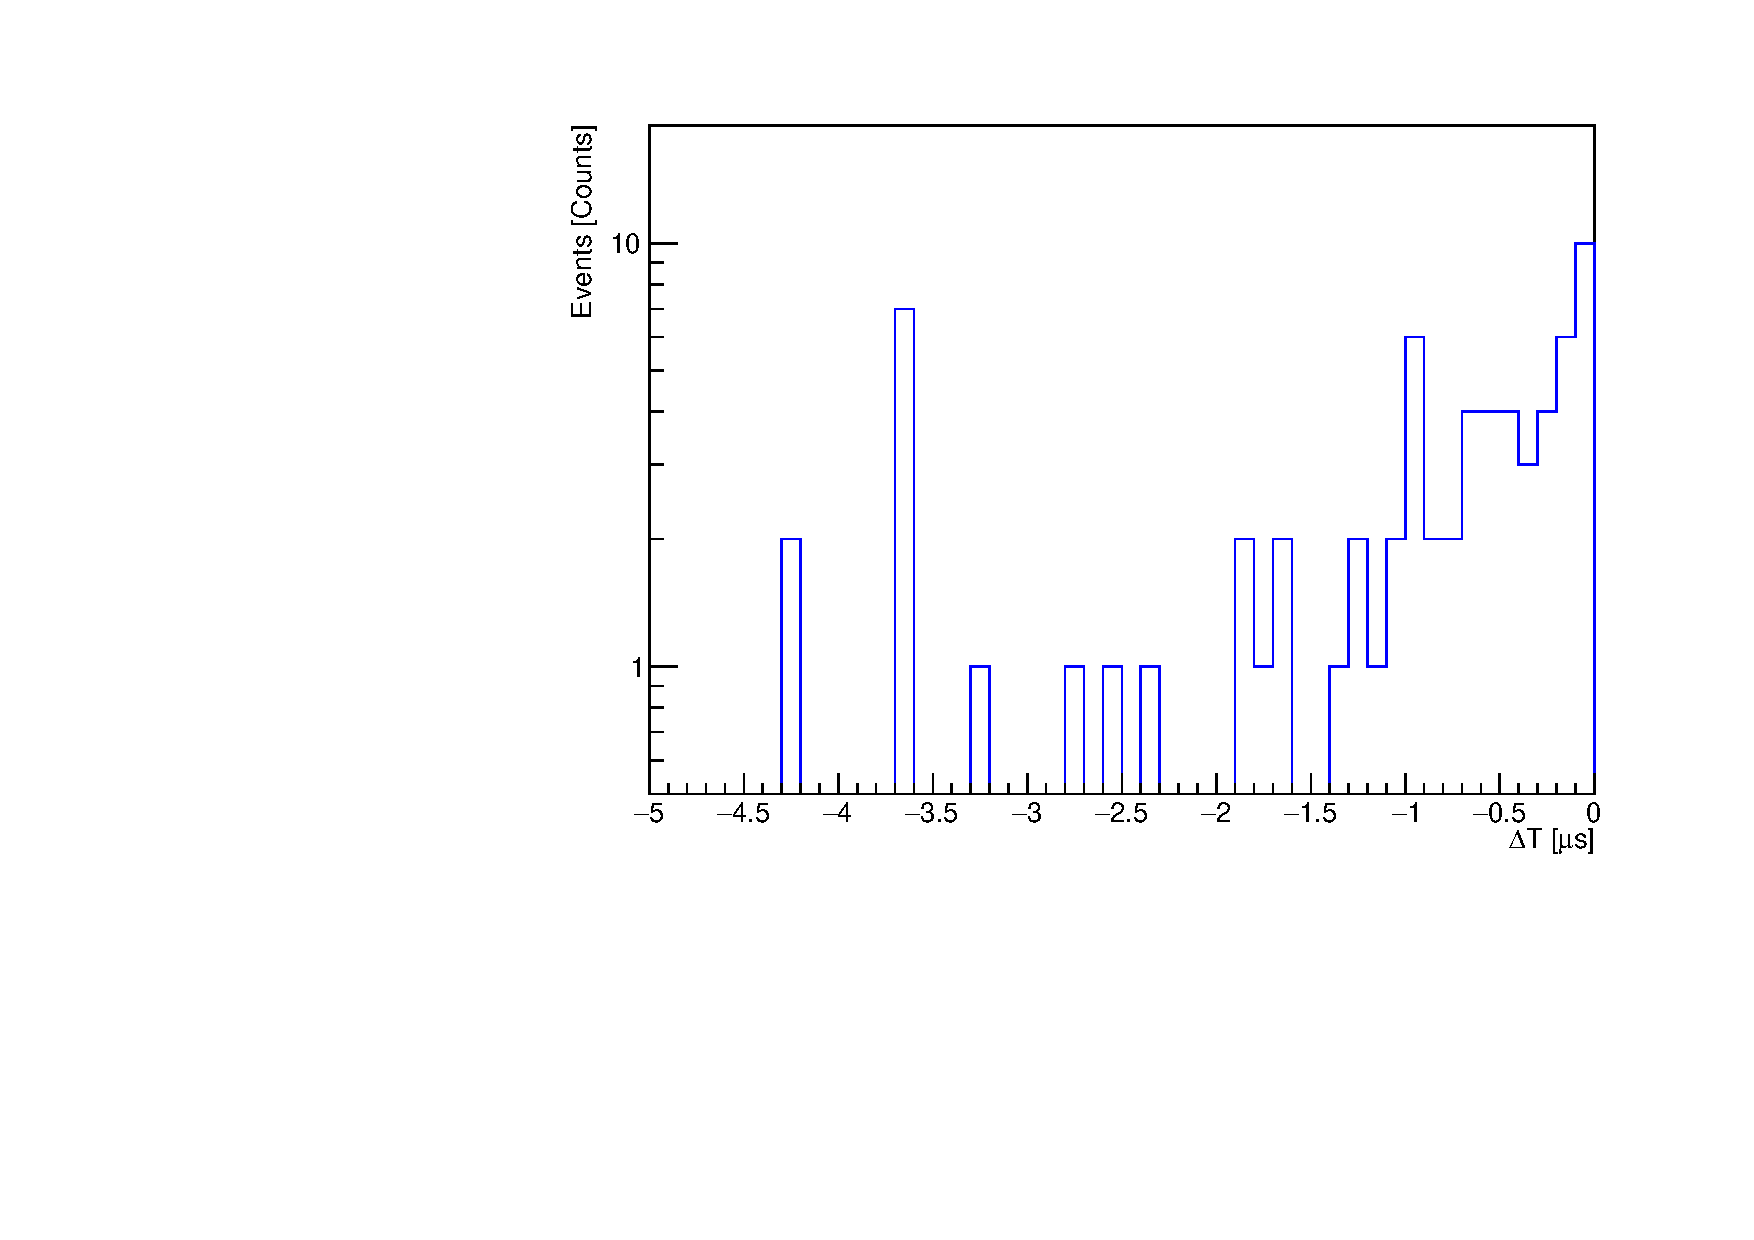
\includegraphics[width=100mm]{./Bilder/TriggerTimeOnly4.pdf}
	\fi%
	\label{fig:Trigger4}
	\caption{
		All liquid argon filtered events with a negative time difference between the event in the Germanium detector and a signal in the photomultipliers in the liquid argon tank.
	}
\end{figure}
Applying these two restrictions to the LAr veto filtered events and from those  only using those photomultiplier events with a signal strength of at least 0.5 phe results in a distribution as shown in Figure \ref{fig:Trigger4}.
Only the signals that have measured at least 0.5 phe are of interest because they have had the necessary intensity to trigger the LAr veto. 
The x axis is the time difference of the events in the photomultipliers from the signal measured in one of the Germanium detectors.
Theoretically it should now be possible to see a exponential increase from the negative scale towards a vanishing time difference.
But due to the small number of events, it is basically impossible to make any statements about the course of these events.
\\

Nevertheless, the number of events of interest was reduced from 1728 to only 55.  
These remaining events can now be manually examined with a software called GerLa.
This tool allows you to search for a specific event and see all recorded signals of the Germanium detectors and the photomultipliers around the time frame of this event.
\\

With this program one can now perform a manual filter by looking at the remaining 55 events individually and perform a specific procedure to determine whether they are signals from a \Kr decay or not.
This procedure consists of filtering out every event that has a combined light intensity of over 5 phe and every event that only has a negative time difference in a signal weaker than 0.5 phe.
The upper limit of the light intensity comes from the fact that the mean kinetic energy of the electron released from the decay is 47.65keV.
With an effective scintillation yield of the whole setup of about 60 phe/MeV one can expect about 2.5 photons from a mean beta electron. 
It can then be assumed that the predominant part of all betas released in the investigated decay only emit 5 photons at best.
\\

\begin{figure}[t!]
	\centering
	\ifmakefigures%
	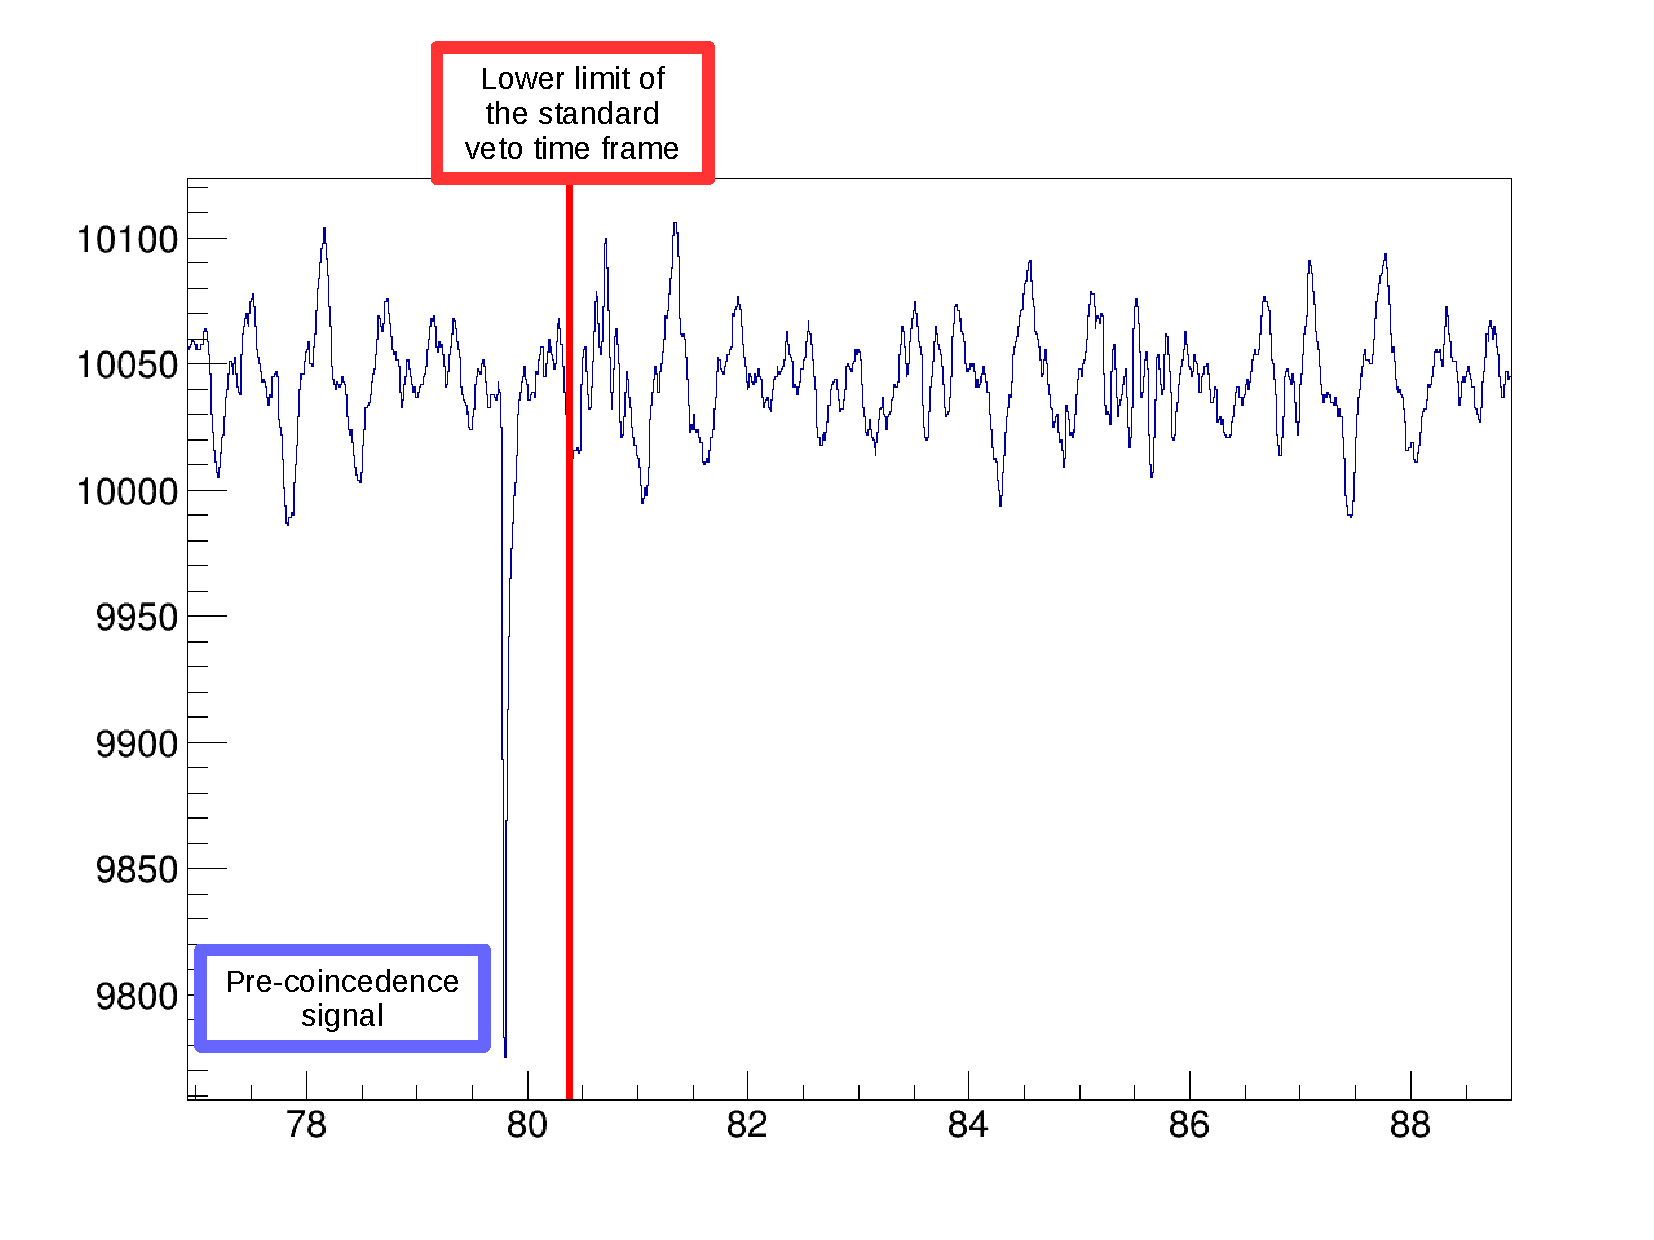
\includegraphics[width=100mm]{./Bilder/BeispielSignal.pdf}
	\fi%
	\label{fig:Trigger4}
	\caption{
    The recorded signal of the photomultiplier tube P4 from the event with event number 1614036. !!!!!Hier noch was zu den Achsen!!!!!. 
    The blue bar represents the moment in time in which a signal in the Germanium detector was measured.
	}
\end{figure}

At this point we realized that this procedure does not really work as well as we hoped it would.
From the remaining 55 only a few events really were unambiguous enough that one could claim that they are the photons we expected.
After this much filtering we can assume that probably all of these events are in fact caused by a \Kr decays.
Signals like the one shown in figure \ref{fig:Trigger4} are a rare example of an almost model signal that we wanted to see.
The great majority of other events were either background events in the SiPM that randomly triggered the LAr veto or their measured signal was too strong.  
\\

With this it was now determined that the majority of events with a negative time difference are in fact not caused by a \Kr decay.
This means that the remaining \Kr decay events must have a positive time difference.
But it is practically impossible to recover them from there due to the great amount of individual events that have to be looked at.
Our recovery attempt has therefor failed.
\\

Nevertheless we are still able to make some qualitative estimations about why approach did not work. 
The major problem seems to be that the majority of events detected with a negative time difference are background events.
This conclusion came from the fact that almost none of the events investigated have shown the expected features we expected from them. 
That the majority of the negative time difference photomultiplier events seem to be background noise is also underlined by the fact that most of these were detected in the PMT. 
As it will be seen in the next chapter, basically all of the decays that created a measurable 514keV event have happend in the vicinity of the detectors themselves an therefor mostly in between the arrays.
The detectors themselves should already block the light of the scintillation relativly strongly but when a photon is detected in a photomultiplier it would most likely be a SiPM.
This is because the fibers surrounding  the germanium detectors are more likely to absorb and guide the scintillation light to the SiPM than a photon to reach a PMT above or below the detector arrays.
Now that the majority of the detected light events are measured in the PMTs it is very unlikely that these are caused by a \Kr decay.
This might also be able to be seen from figure \ref{fig:AntiLArBEGes} and \ref{fig:AntiLArCOAX}.
In those all filtered out events are shown over the measured energy.
From it we first saw that the liquid argon veto also filtered out the wanted 514keV events.
But from it we can also see, that the ratio of events filtered out at the 514keV mark over the non filtered value [$N_{\unit{vetoed}}(514\unit{keV})/N_{\unit{unfilered}}(514\unit{keV})]$ is about the same size as in a non peak area whereas the positron electron peak shows much higher ratio.
Considering this the peak probably came to be because the same relative amount of events have their liquid argon veto triggered because of background events.
It is therefor rather questionable whether the liquid argon veto is even a good filter to use when it also filters out events in which background can trigger the veto too.
A satisfactory answer however will only be available through a quantitative analysis which will be performed in the following chapter.
\\

\section{Fitting}
\label{sec:Fitting}

Our strategy to calculate the activity of \Kr through the 514keV peak involves determining the absolute amount of measured \Kr decays events over all of \PII.
Due to the still enormous amount of events from other sources that can not be suppressed, for example the \nuc{Ge}{76} decays, it is necessary to fit the 514keV peak with a suitable fit function.
The amount of measured \Kr decay events can then be calculated by integrating over the found fit function and dividing by the probability of the specific decay into \nuc{Rb}{85m}.
\\

The not liquid argon filtered spectrum \ref{fig:NoFilterBEGes} and \ref{fig:NoFilterCOAX} show two peaks.
This requires the fit function to include two Gaussian functions from which only the parameters of the second peak will then be analyzed.
Additionally to the two Gaussian peaks a constant and an exponential background function will be added.
When looking at the not liquid argon filtered spectra again we can see that over the course of the displayed interval no real change in count rate over energy can be seen (see figure \ref{fig:NoFilterBEGes} and \ref{fig:NoFilterCOAX}).
But theoretically we expect the distribution of the germanium events to behave like its phase-space function and therefor change with energy.
It is therefor necessary to also consider this change in count rate over energy in the fit function.
The phase-space function of \nuc{Ge}{76} is very complex however.
In this case however is the energy interval relatively small compared to the complete spectrum of \nuc{Ge}{76}.
This allows the approximation that its phase-space function changes like an exponential decrease due to the general form of the measured spectrum in this energy range.
The resulting fit function is shown in equation \ref{equ:FitNoFilters}.
\\

\begin{equation}
\mathrm{f}(x) = \mathrm{A}\frac{1}{\sqrt{2\pi}\mathrm{C}}\exp\left(-\frac{(x-\mathrm{B})^2}{2\mathrm{C}^2}\right) + \mathrm{D}\frac{1}{\sqrt{2\pi}\mathrm{F}}\exp\left(-\frac{(x-\mathrm{E})^2}{2\mathrm{F}^2}\right) + \mathrm{G}\exp\left(\mathrm{H}x\right) + \mathrm{I}
\label{equ:FitNoFilters}
\end{equation}
\\

In the course of the fitting process it has to be mentioned that some fitness parameters have only been left free for rather small interval.
Most notably the values C and F, being the variances of two Gaussian peaks, were each only left free on a very small range around the values derived from the resolutions of the detectors at their specific energies (see appendix section \ref{sec:ResDetermination}).
When you apply the fit function to the two different spectra of the two kinds of detectors you get the graphs displayed in figure \ref{fig:FitNoFilterBEGes} and \ref{fig:FitNoFilterCOAX}.
The resulting fit parameters are listed in table \ref{tab:FitParNoFilter}. 
\\

\begin{figure}[t!]
	\centering
	\begin{subfigure}{.5\textwidth}
		\centering
		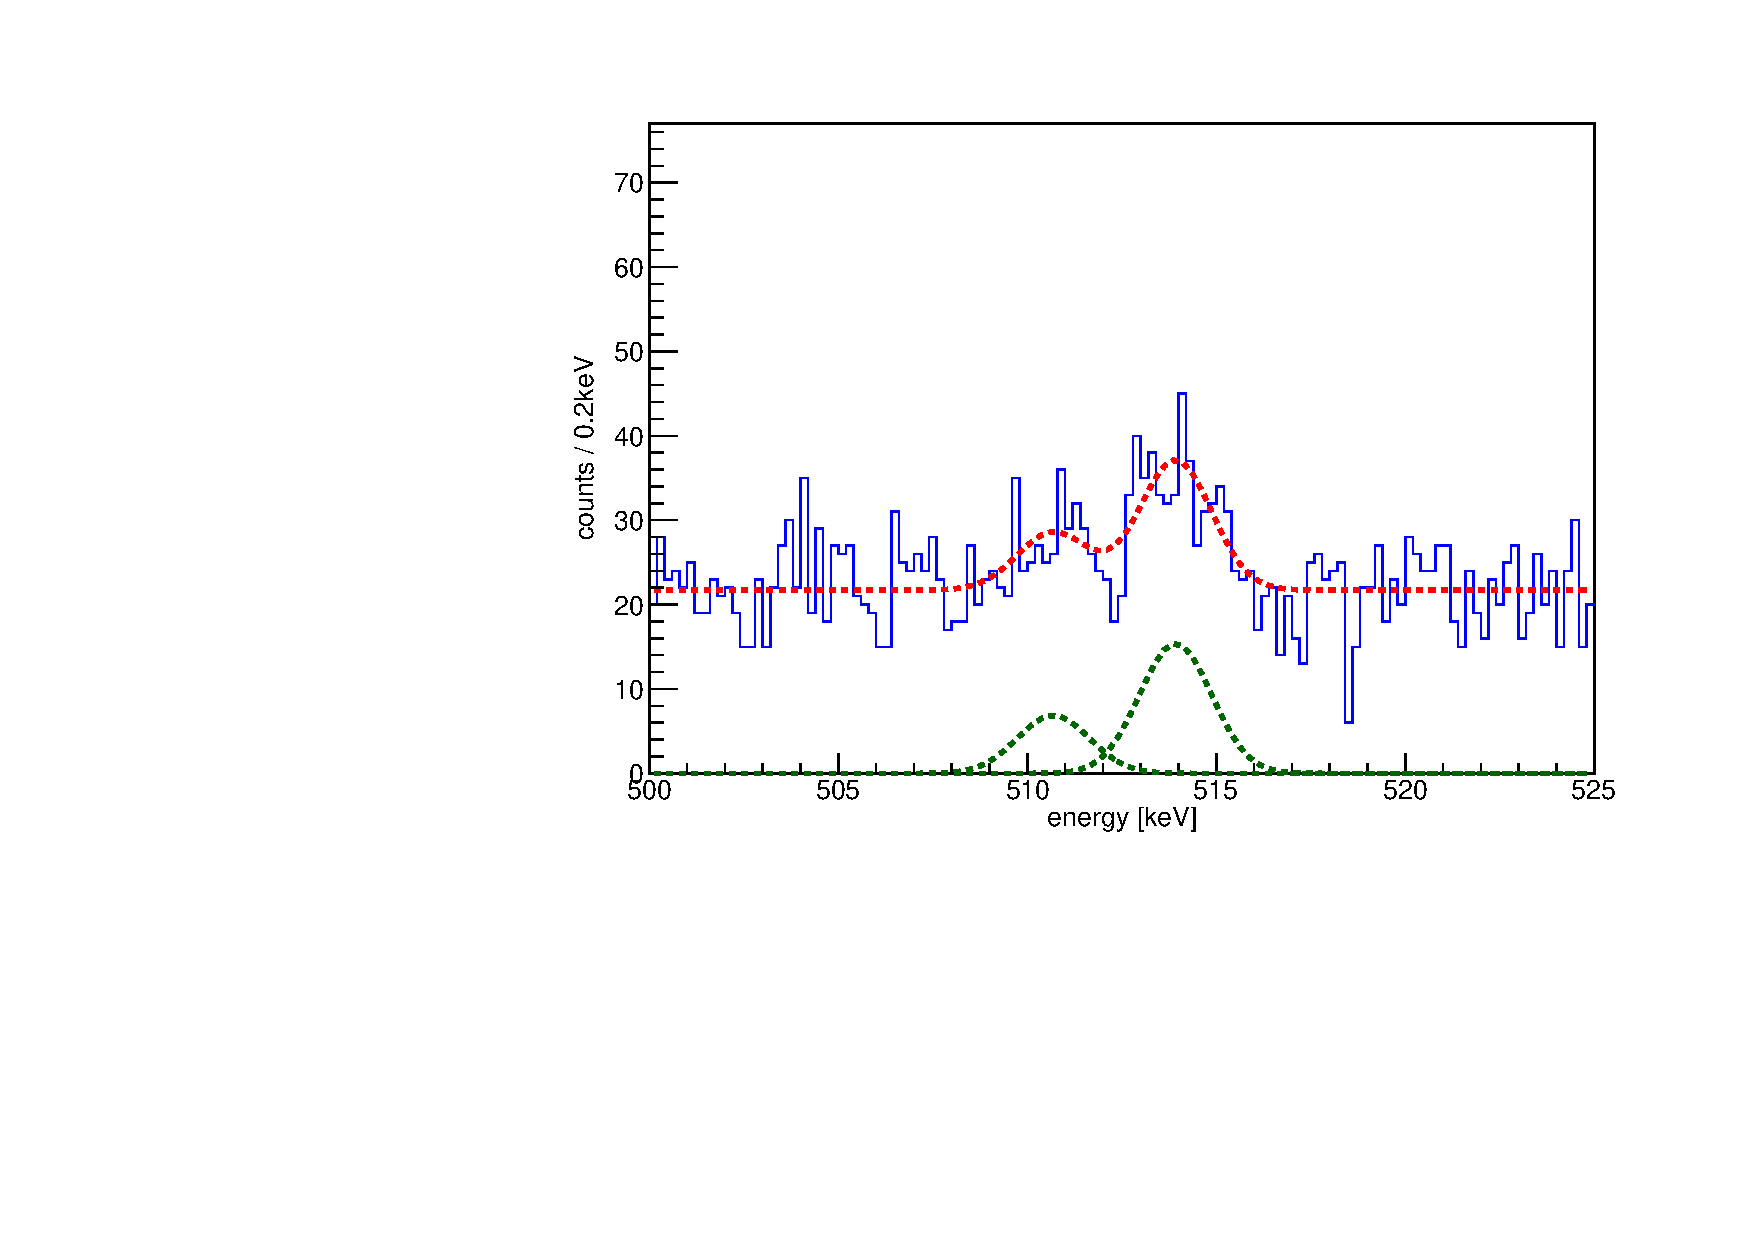
\includegraphics[width=75mm]{./Bilder/500525FitNoFilterBEGes.pdf}
		\caption{BEGes}
		\label{fig:FitNoFilterBEGes}
	\end{subfigure}%
	\begin{subfigure}{.5\textwidth}
		\centering
		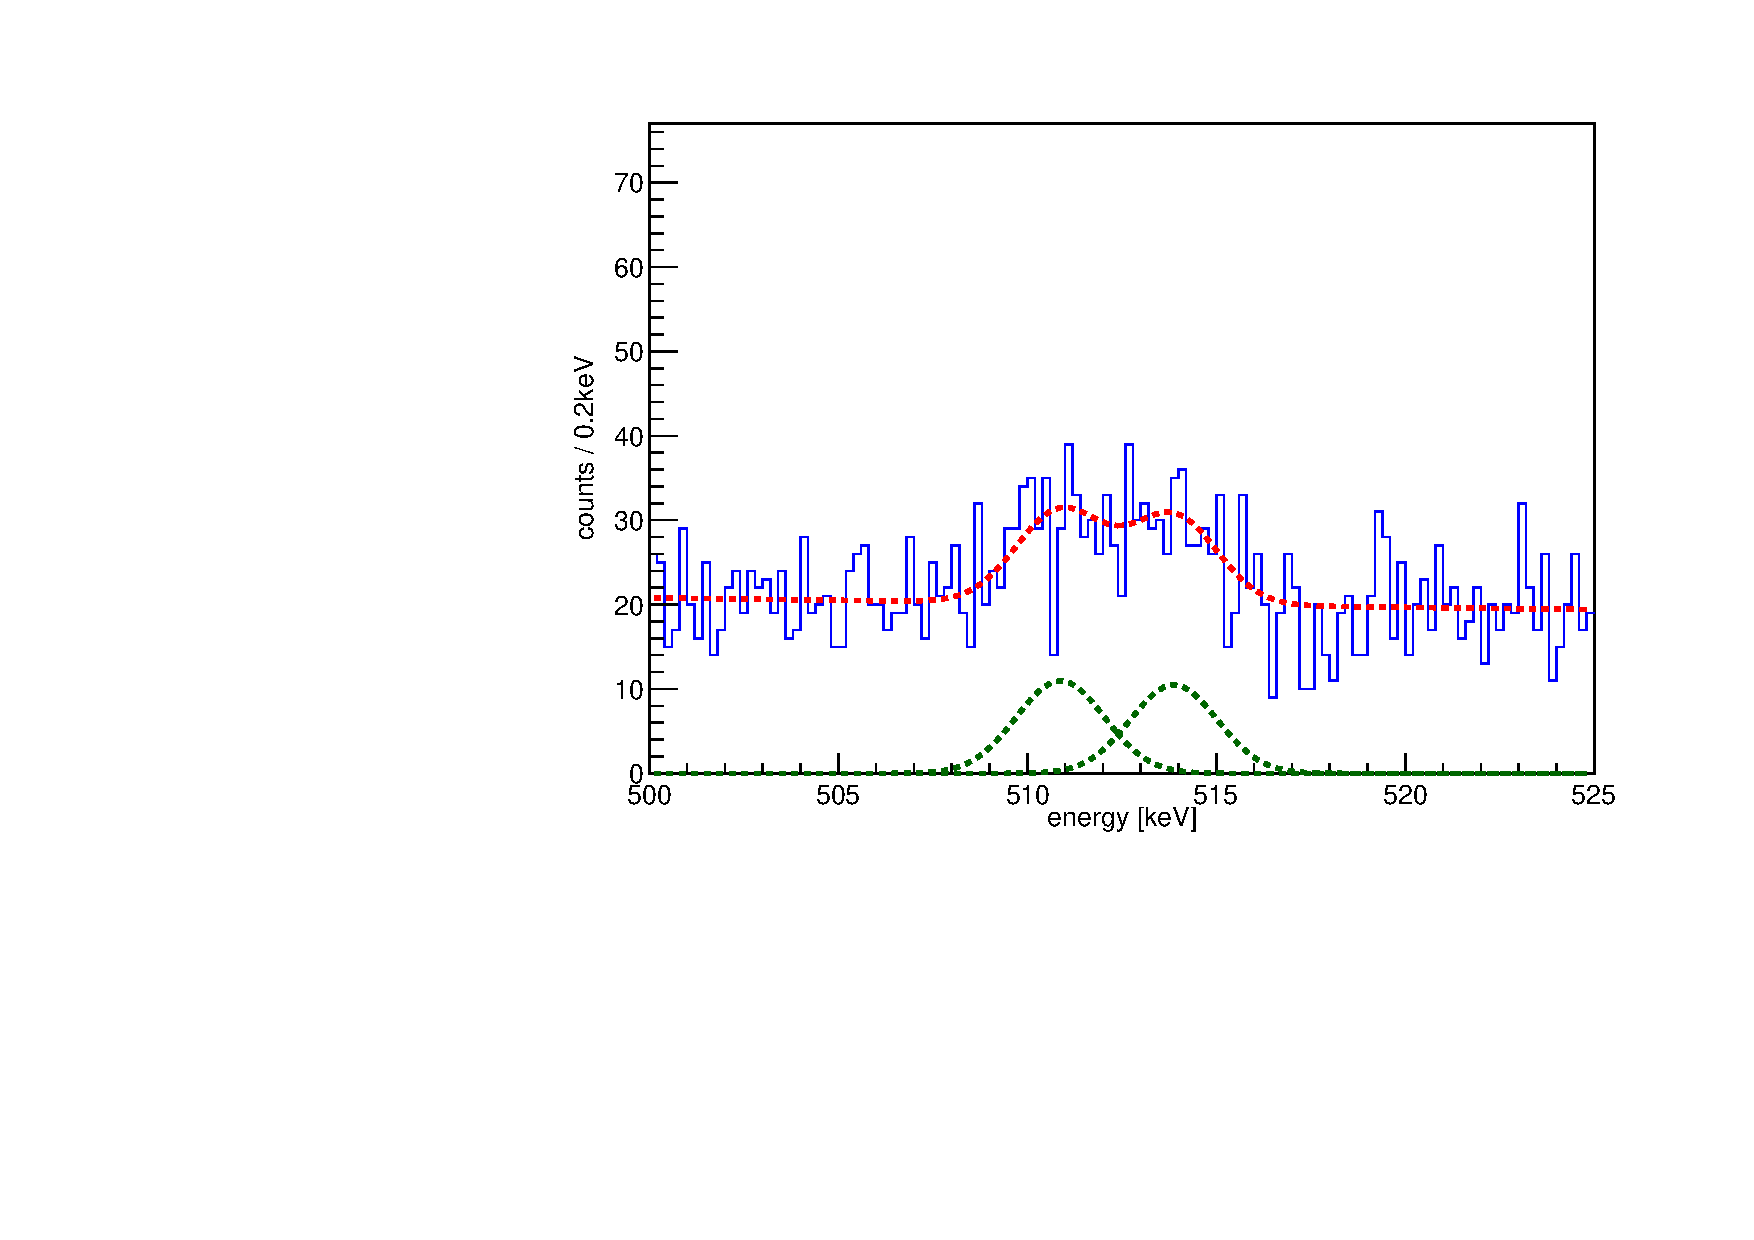
\includegraphics[width=75mm]{./Bilder/500525FitNoFilterCOAX.pdf}
		\caption{COAX}
		\label{fig:FitNoFilterCOAX}
	\end{subfigure}
    \\
	\vspace{0.5cm}
	\caption{All events measured by the respective detectors in the range of 500keV to 525keV fitted with a fit function in the form seen in equation \ref{equ:FitNoFilters}. The green function represent the two Gaussian peaks independently using the determined fit parameters.}
\vspace{0.5cm}
\end{figure}
\\

\begin{figure}[t!]
\centering
\begin{tabular}{|c|c|c|}
\hline
Name	& Value [BEGes] & Valuse [COAX]\\ 
\hline
A  &	(16.384684 \(\pm\)	4.229890	)&	(29.842 \(\pm\)	3.968)	\\	
\hline
B  &	(510.689545  \(\pm\)	0.275479	)&	(510.750 \(\pm\)	0.265)\\	
\hline
C  &	(0.952063 \(\pm\)	0.010154	)	&	(1.564 \(\pm\)	0.236	)	\\
\hline
D  &	(36.757652 \(\pm\)	4.743389)	&	(20.463 \(\pm\)	3.279	)	\\
\hline
E  &	(513.923462 \(\pm\)	0.153953	)	&	(513.858 \(\pm\)	0.213)	\\
\hline
F  &	(0.952731 \(\pm\)	0.011750	)	&	(1.017 \(\pm\)	0.173	)	\\
\hline
G  &	(21.714308 \(\pm\)	0.432063)	&	(13.123 \(\pm\)	0.289	)	\\
\hline
H  &	(-224175.656250 \(\pm\)	0.000424)	&	(-384995.062 \(\pm\)	2.592)	\\
\hline
I  &	(-0.655847 \(\pm\) 0.399776)	&	(-40.573 \(\pm\)	1.414)\\
\hline

\end{tabular}
\label{tab:FitParNoFilter}
\captionof{table}[]{Fit parameters of fit function \ref{equ:FitNoFilters} applied on the spectra of the respective detectors.}
\end{figure}
\\



The only values of these fit parameters that is of real interest for the determination of the activity is variable D.
Its value is the amplitude of the second Gaussian peak.
Because the Gaussian peak was chosen in the normalized form this value also represents the amount of \Kr decays measured per binning of the histogram.
But we only want the amount of counts in the peak independently of the binning of the histogram.
We therefor have to multiply these values with $\frac{1}{0.2}\unit{keV}$.
Finally, we can conclude that in the BEGes an amount of !!!!! events was measured and in the COAX detectors a number !!!!! of events.
\\


From the fit parameter value H and I we can also see that as expected the change of the background over the inspected energy interval is neglactable.
Parameter I defines the change in energy and its value so small that the exponential function in the range that is investigated in has no real impact on the overall fit function.
But as mentioned before it would have been wrong to leave out the fit functions possibility to change over energy because otherwise it might have ruined our whole fitting process. 
\\


After finding the fit parameter for the not liquid argon filtered spectrum we now go to the filtered spectrum.
As mentioned above we can assumed that the positron electron annihilation peak is fully suppressed.
Additionally in the ideal case, that the majority of all \Kr decay events got through the liquid argon filter, we expect the amplitude of the Gaussian peak to be similar to the amplitude in the not liquid argon filtered case.
Therefor only one Gaussian peak has to be fitted together with the background function.
The fit results in the function displayed in equation \ref{equ:FitFilters}.
\\ 

\begin{equation}
\mathrm{f}(x) = \mathrm{A}\frac{1}{\sqrt{2\pi}\mathrm{C}}\exp\left(-\frac{(x-\mathrm{B})^2}{2\mathrm{C}^2}\right) + \mathrm{D}\exp\left(\mathrm{E}x\right) + \mathrm{F}
\label{equ:FitFilters}
\end{equation}
\\

After applying the fit to the spectra seen in figure \ref to \ref, you get the fit parameters displayed in table \ref.
As above, the amplitude A of the Gaussian peak correspond to the number of events measured in the area of the peak per binning.
This results in an amount of !!!! for the BEGe and !!!!! for the COAX spectrum.
As mentioned above these values are only planned to be a crosscheck for the not argon filtered values. 
Compared to those values, it can be seen that the number of events in the BEGe and in the COAX detectors has dropped considerably.
This means that some of the \Kr decay events must have been filtered out and a recovery of these falsely filtered \Kr decays is necessary.
But due to that not being possible we can not use those results in our analysis nor for a real crosscheck..
\\

\begin{figure}[t!]
	\centering
	\begin{subfigure}{.5\textwidth}
		\centering
		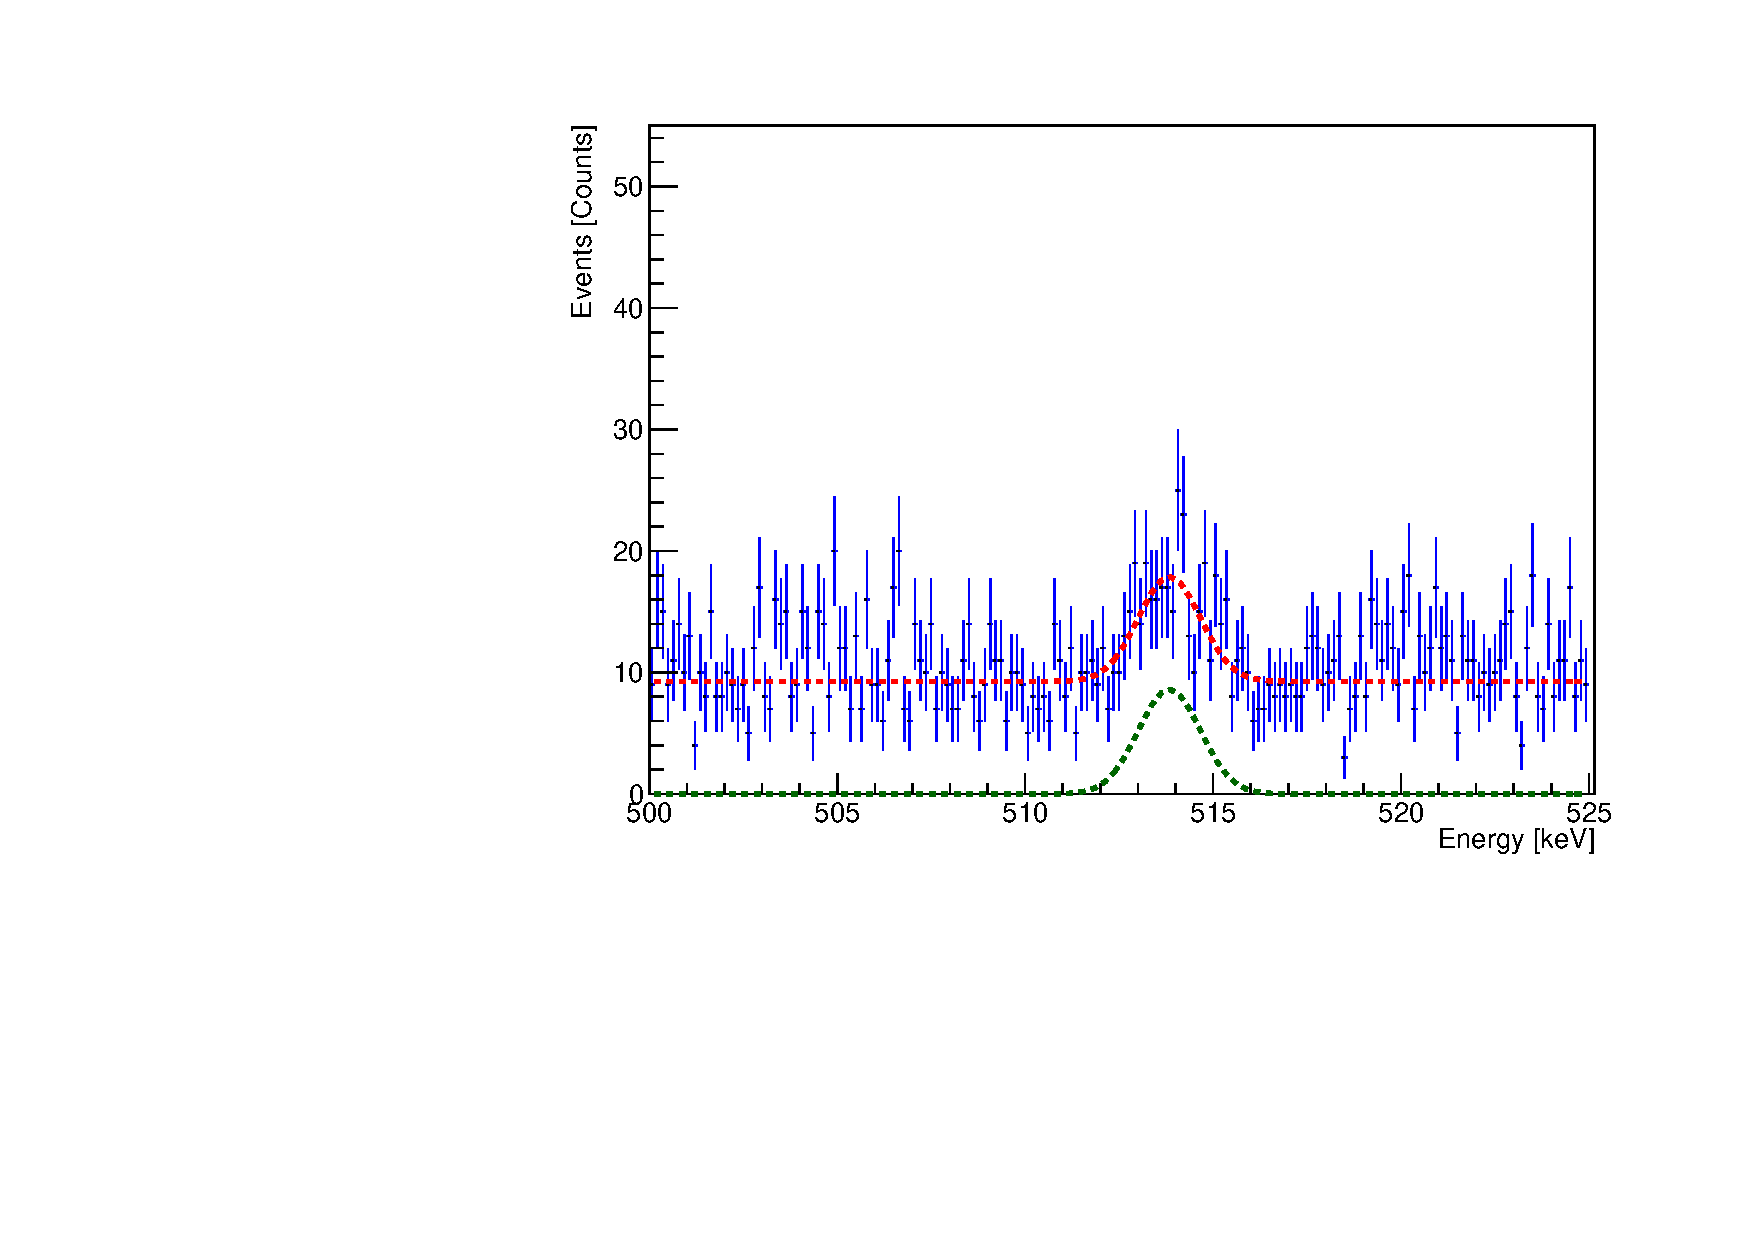
\includegraphics[width=75mm]{./Bilder/500525FitLArVetoBEGes.pdf}
		\caption{BEGes}
		\label{fig:FitLArVetoBEGes}
	\end{subfigure}%
	\begin{subfigure}{.5\textwidth}
		\centering
		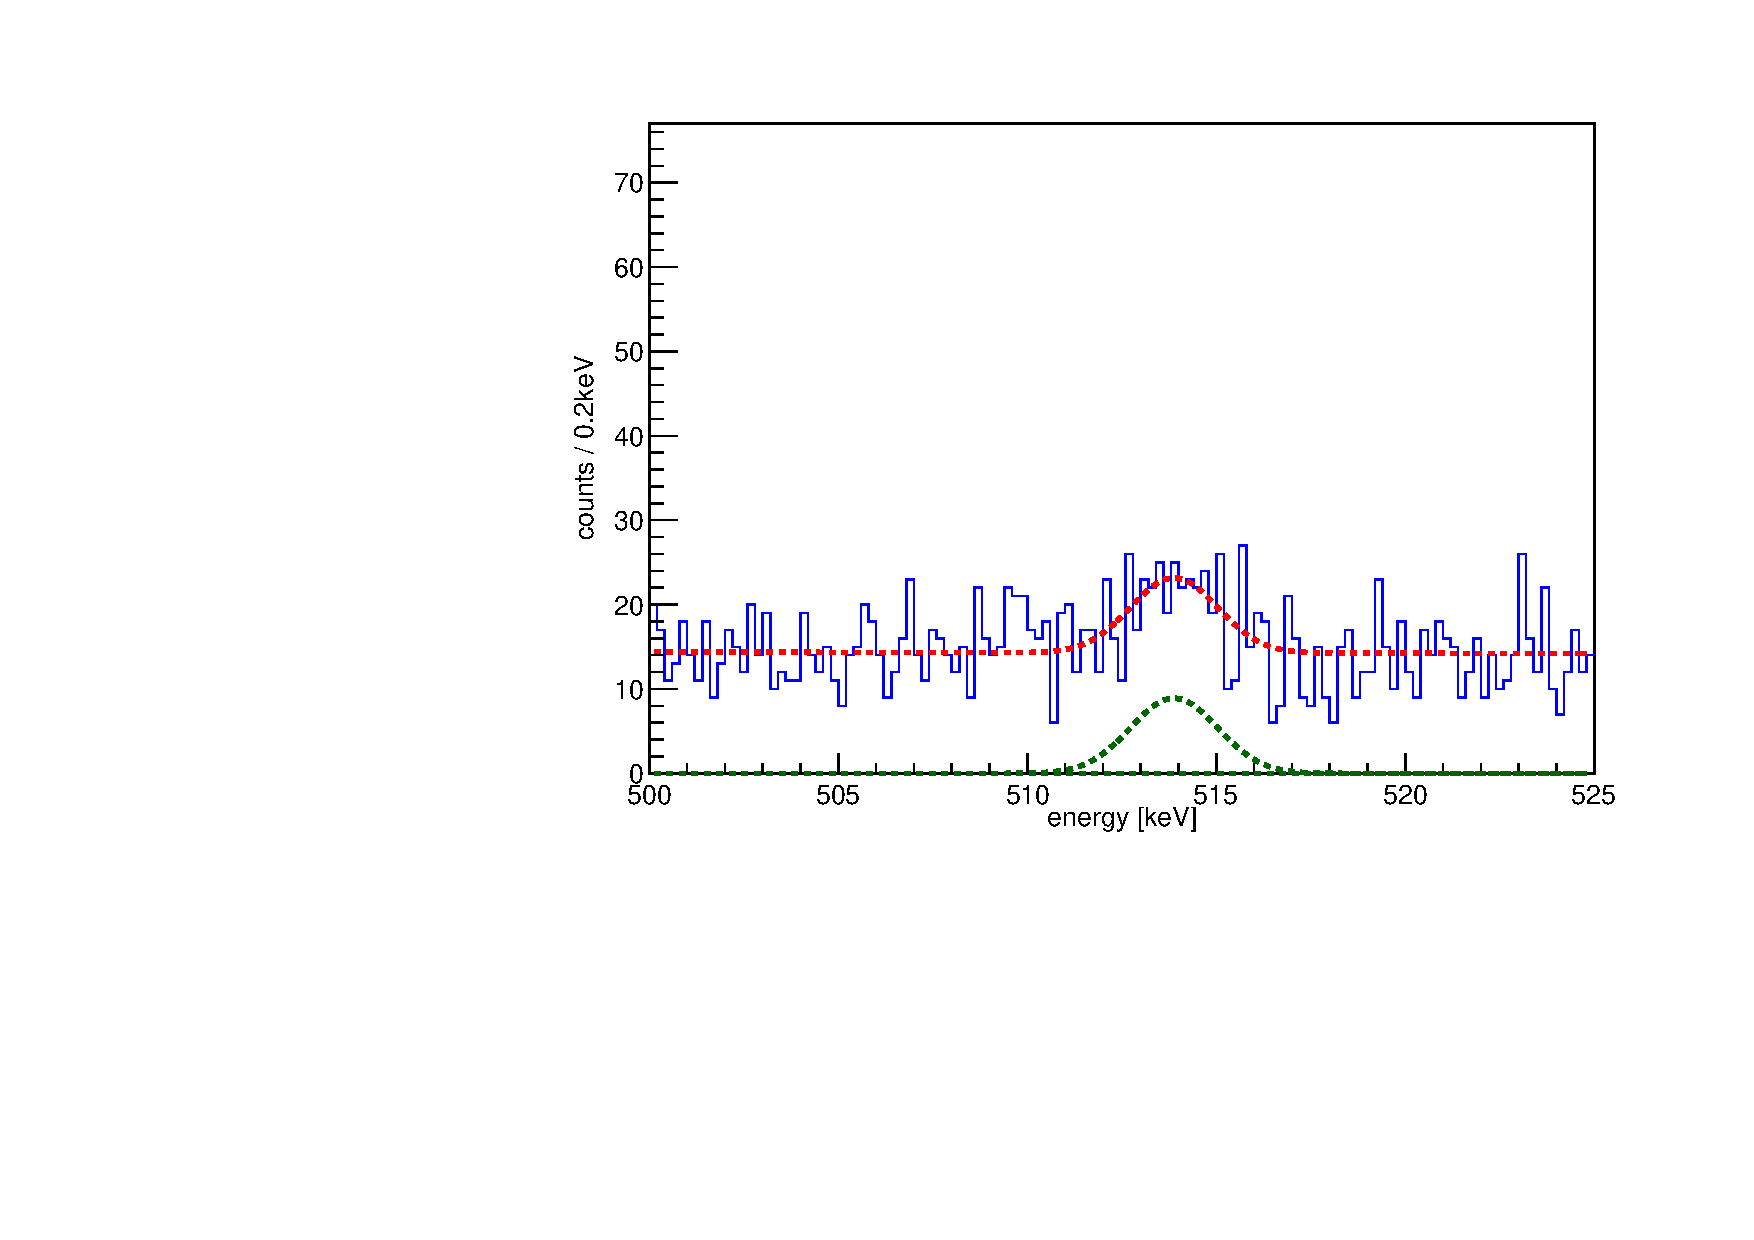
\includegraphics[width=75mm]{./Bilder/500525FitLArVetoCOAX.pdf}
		\caption{COAX}
		\label{fig:FitLArVetoCOAX}
	\end{subfigure}
	\caption{All events measured by the respective detectors  with the liquid argon veto applied in the range of 500keV to 525keV fitted with a fit function in the form seen in equation \ref{equ:FitFilters}.}
\end{figure}

\begin{figure}[t!]
	\centering
	\begin{tabular}{|l|r|r|r|r|}
		\hline
		Name	& Value [BEGes] \\ 
		\hline
		A  &	(17.844639 \(\pm\)	3.179471)&	(17.914476 \(\pm\)	2.683260)	&	(19.847330\(\pm\)	2.688415)&	(18.851511 \(\pm\)	2.696000)\\	
		\hline
		B  &	(513.838989 \(\pm\)	0.665171)&	(513.748535 \(\pm\)	0.179167)&	(513.849854 \(\pm\)	0.152052)&	(513.737183	\(\pm\) 0.167941)\\	
		\hline
		C  &	(0.828315 \(\pm\)	1.377836)	&	(0.940856 \(\pm\)	0.160788	)	&	(0.865958\(\pm\) 0.108436)&	(0.923679 \(\pm\)	0.149867)\\
		\hline
		D  &	(9.265341 \(\pm\)	1.032088)	&	(9.073170 \(\pm\)	0.233725	)	&	(9.307535\(\pm\)	0.236841)&	(9.076473 \(\pm\)	0.233940)\\
		\hline
		E  &	(18.142975 \(\pm\)	1.833031)	&	(-401772.843750 \(\pm\)	3.666062)	&	(-394189.968750\(\pm\)	45.660984)&	(-796827.062500 \(\pm\)	64.574379)\\
		\hline	
		F  &	(-26.647284 \(\pm\)	1.000000)	&	(-43.877174 \(\pm\)	1.414214	)	&	(-55.546192\(\pm\)	1.414214)&	(-55.546192 \(\pm\)	1.414214)\\
		\hline
	\end{tabular}
	\label{tab:FitParNoFilter}
	\captionof{table}[]{Fit parameters of fit function \ref{equ:FitNoFilters} applied on the spectra of the respective detectors.}
\end{figure}

Now that we have a number of the special \Kr events measured in the respective detectors.
But what we need for the determination of the activity is not the amount of measured events but actually the amount of \Kr decays in the whole liquid argon tank.
Luckily we can calculate the amount of actual events in the liquid argon tank by determining the detector efficiency of the two detector types.
This can be done by running a Monte Carlo simulation simulating a great amount of 514keV photon emissions in a cylindrical volume with a detector therein with the same design as used in GERDA.
From the amount of measured events in these simulated detectors and the absolute amount of simulated events one can then calculate the efficiency with which the detectors measure any \Kr events. 
How exactly this was implemented is the topic of the next chapter.
\\

\section{Monte Carlo Simulation}
\label{sec:MonteCarlo514}

As described above, we want to determine a conversion factor between the measured 514keV events and the decay density of \Kr necessary to create this signal.
Such a conversion factor can be determined with the help of a Monte Carlo simulation.
The tool used to perform this simulation is \mage (MAjorana-GErda), a GEANT4-based physics simulation software developed jointly by MAJORANA and GERDA \cite{boswell_mage_2010}.
Both experiments aim to measure the neutrinoless double beta decay using enriched Germanium detectors.
Because it is expected that the halflife of this decay is in the order of at least \(10^{25}\) years, a lot of effort is put into finding out how big the contribution of different isotopes to the background is.
\mage is therefor specialized to simulate radioactive decays and their corresponding measured events in Germanium detectors.
\\

The simulation used here consists of a cylindrical of 2.5m of height and 3m in diameter, in which the detector structure of the GERDA experiment is placed in the middle.
The resulting volume of the liquid argon is $V_{sim} = 17.65 \mathrm{m}^3$ .
Compared with the volume of 64 m\(^3\) of liquid argon used in the GERDA experiment this volume is much smaller.
But as we will see later, this volume is by far big enough for our purpose.
A total of N = 50.000.000 photons with an energy of 514keV are now simulated in of the volume in this cylinder that is not occupied by the detectors. 
As can be seen in figure \ref{fig:CrossSecAb}, the density of the decays over the entire volume of the cylinder is relatively constant.
\\

\begin{figure}[t!]
	\centering
	\begin{subfigure}{.5\textwidth}
		\centering
		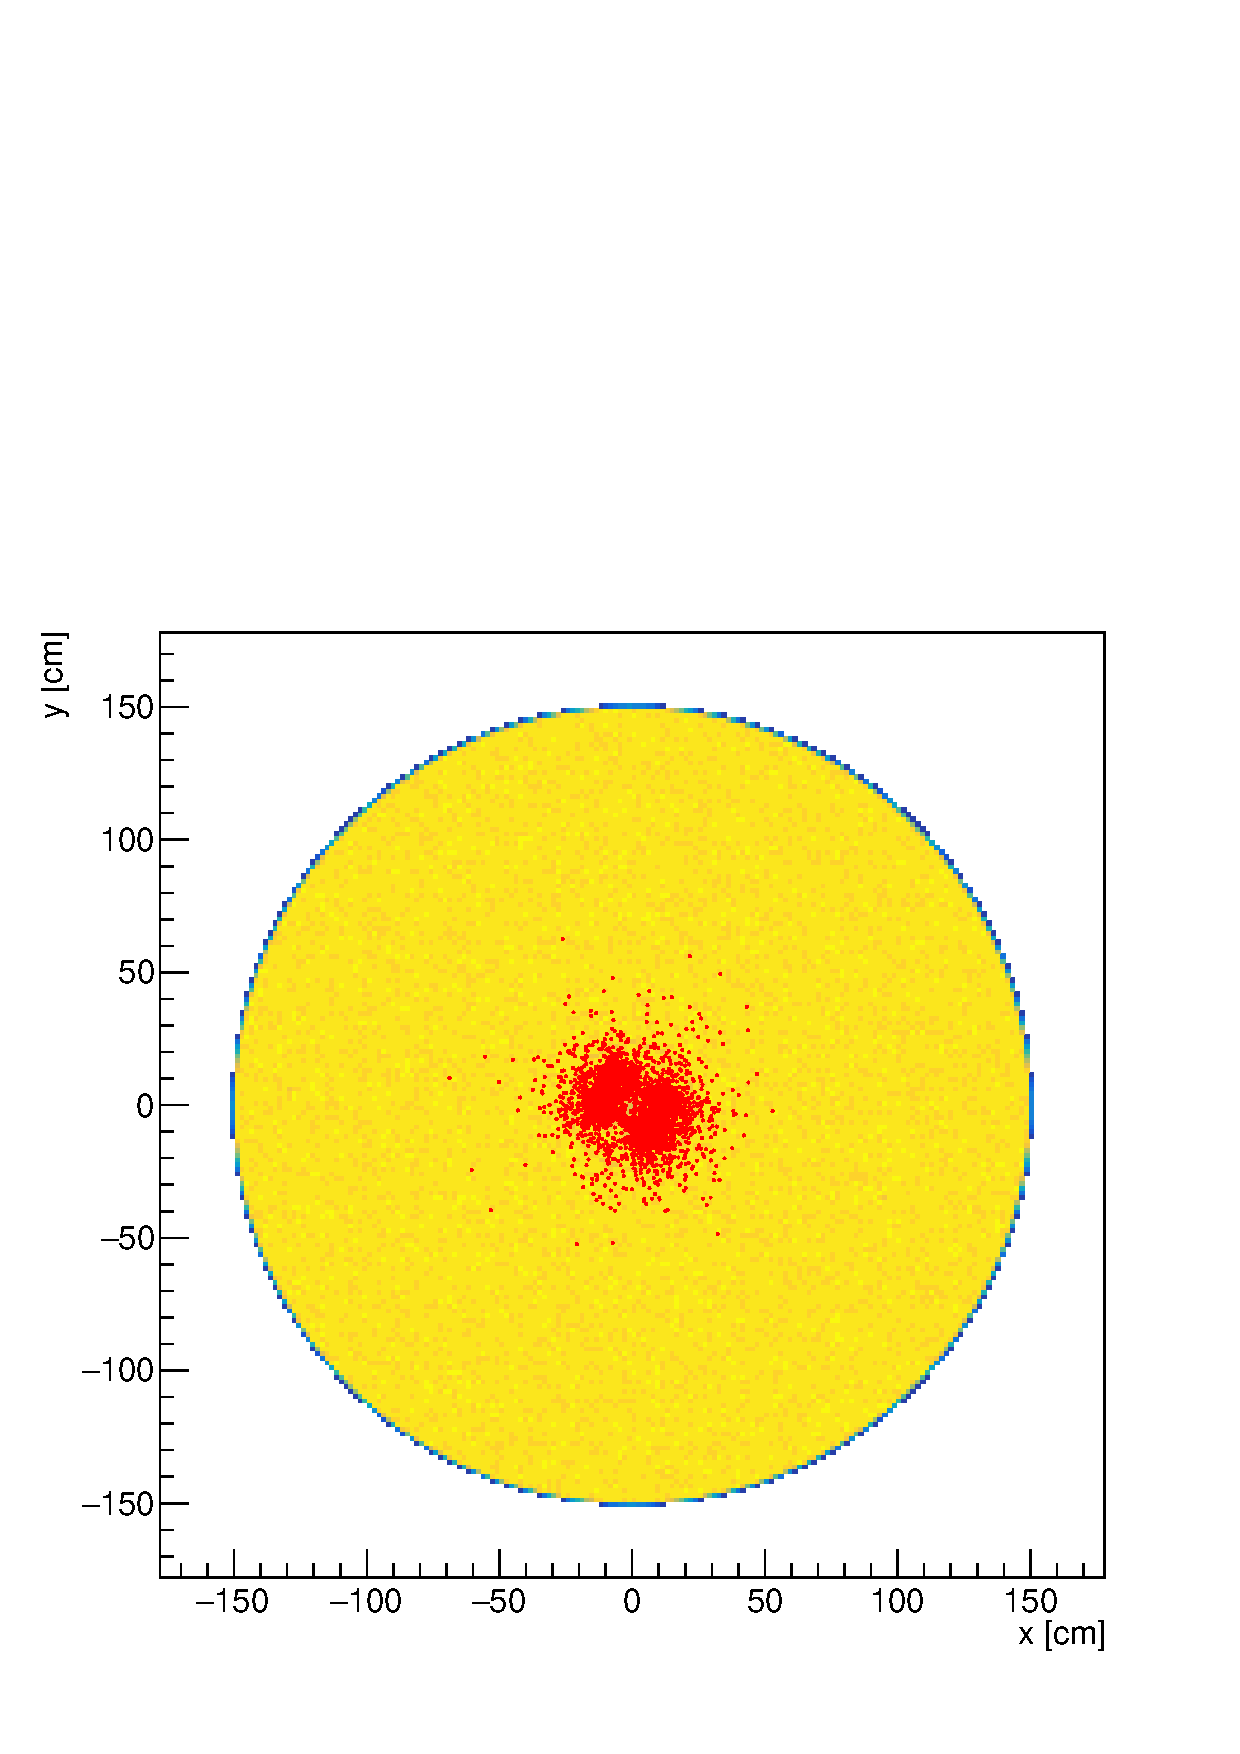
\includegraphics[height=75mm]{./Bilder/MC-Querschnitt-BEGes.pdf}
		\caption{Cross section from above}
		\label{fig:CrossSecAb}
	\end{subfigure}%
	\begin{subfigure}{.5\textwidth}
		\centering
		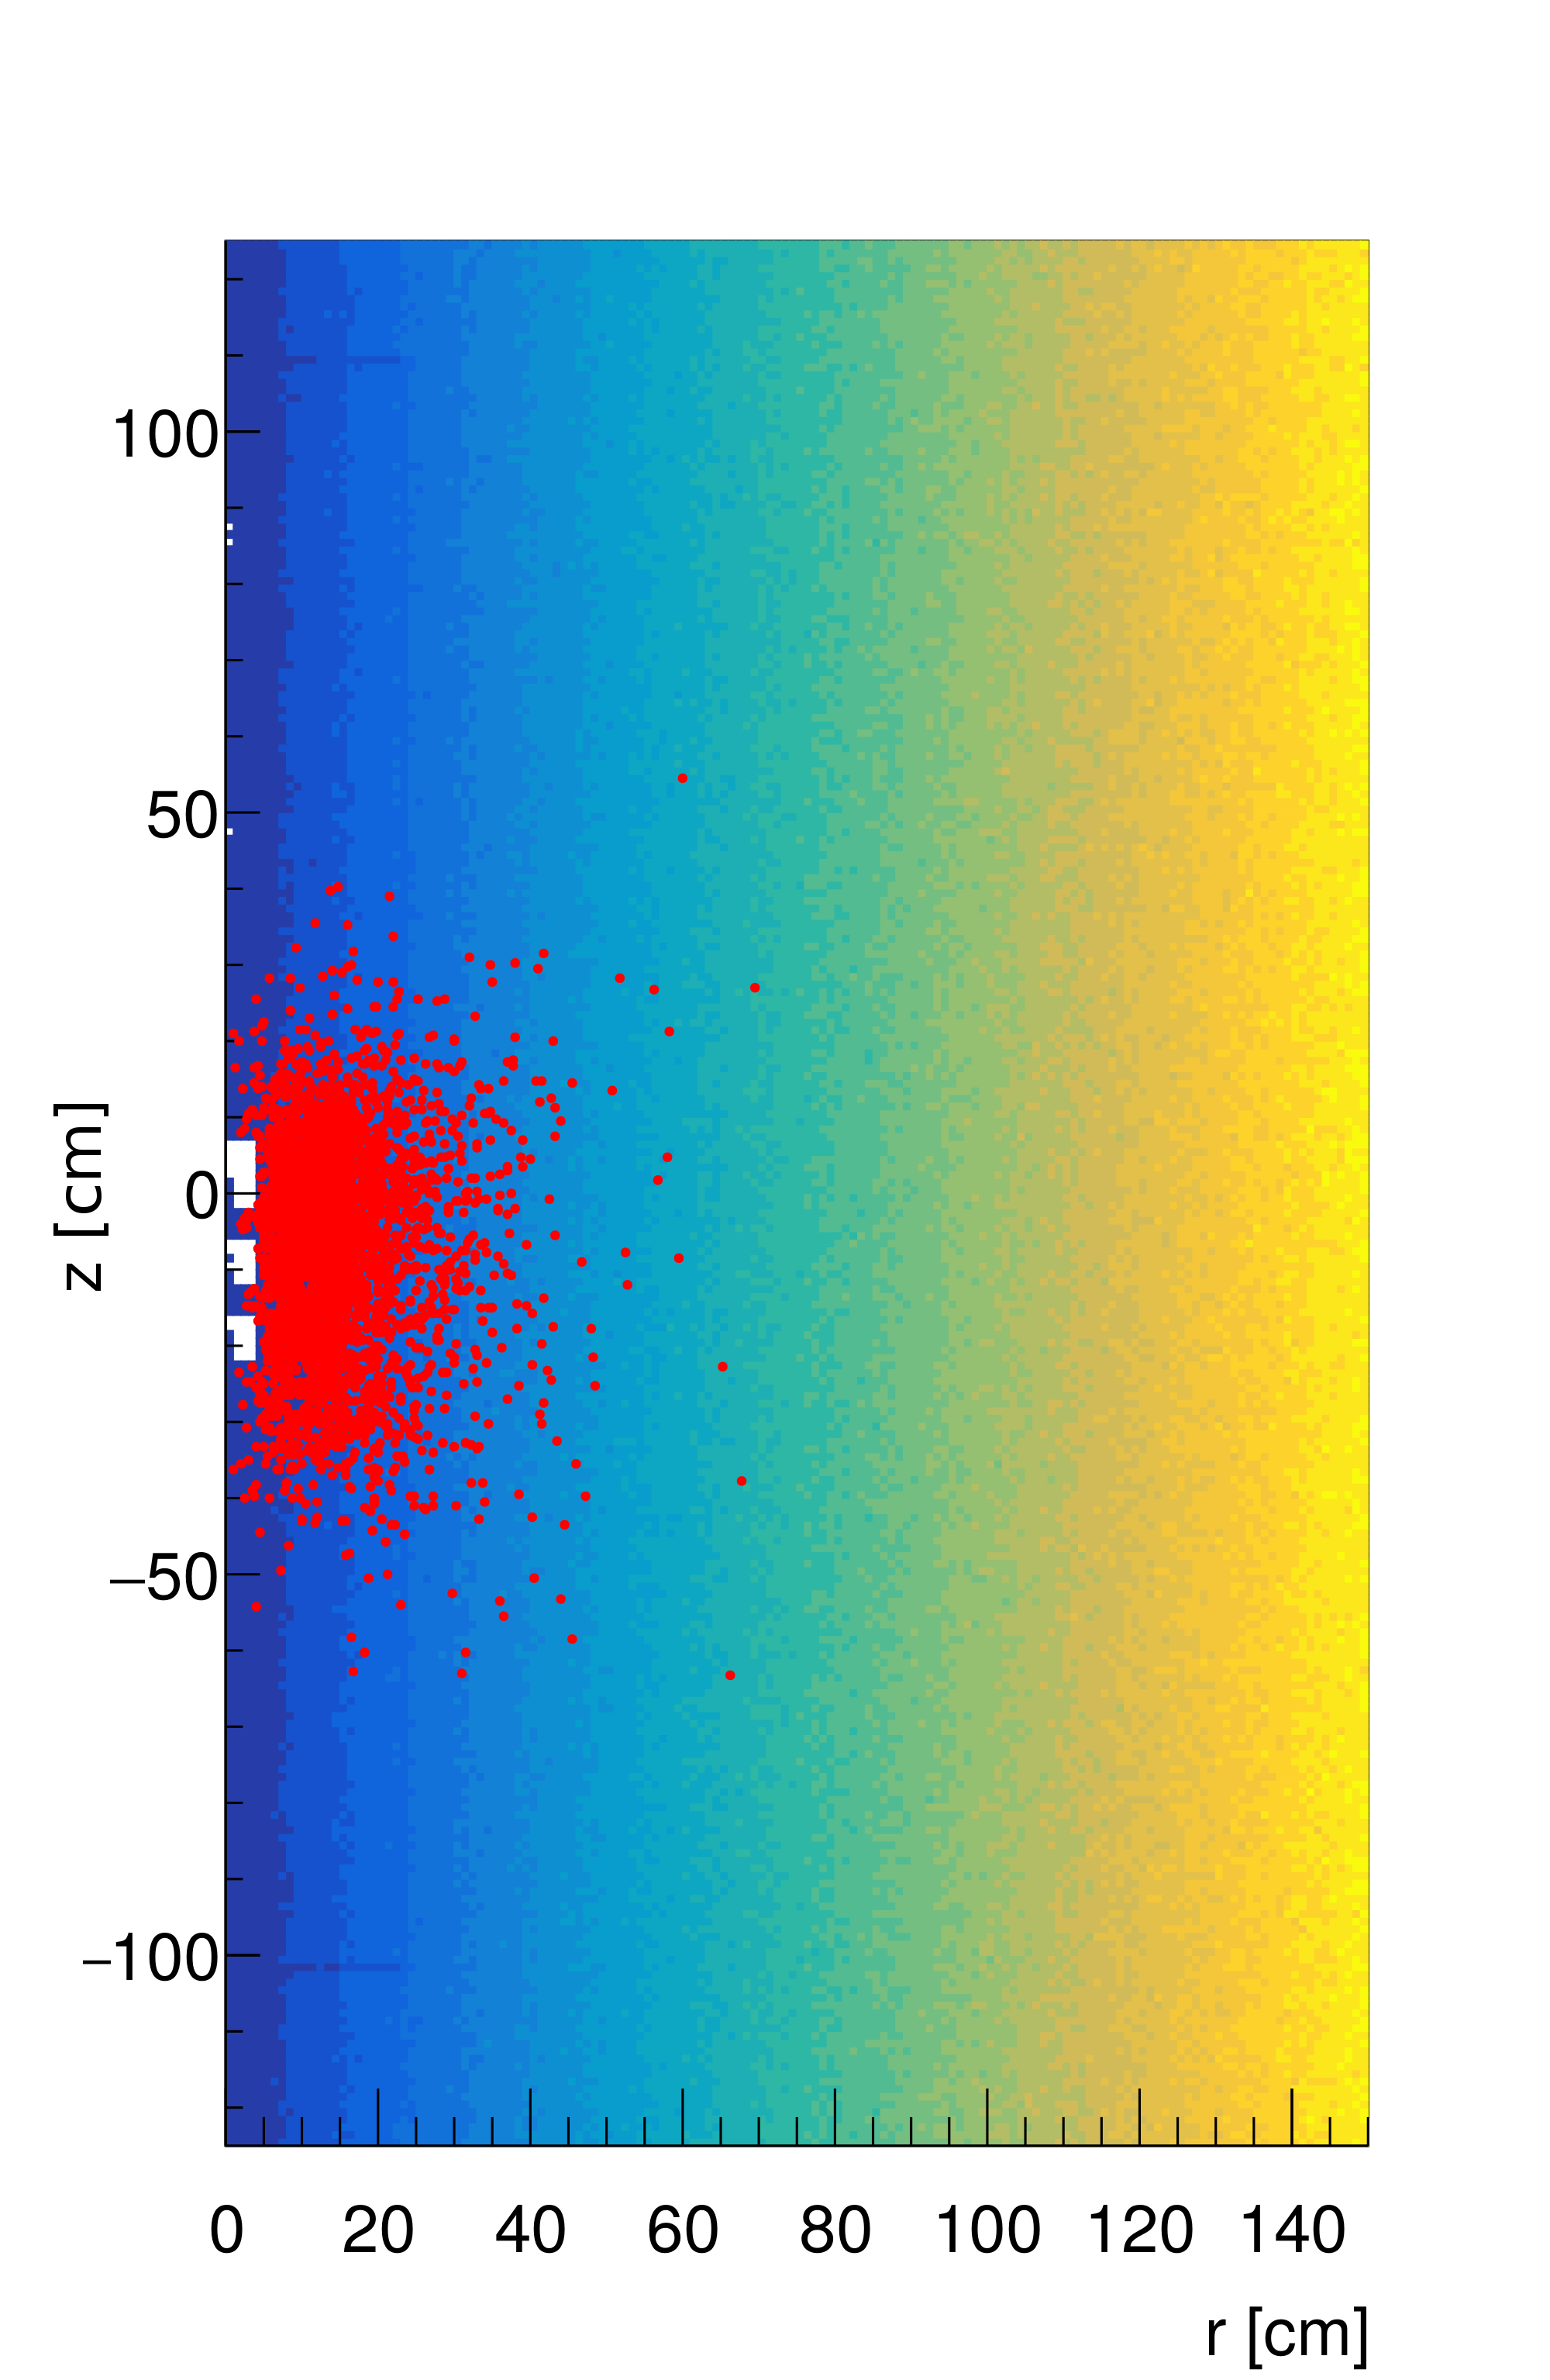
\includegraphics[height=75mm]{./Bilder/MC-Radius-BEGes.png}
		\caption{Radial cross section}
		\label{fig:CrossSecRa}
	\end{subfigure}
    \\
	\vspace{0.5cm}
    \caption{Cross section from above and a radial cross section showing the density of simulated decays in the cylindrical volume. The red points indicate all events that were measured by the BEGe detectors.}
\vspace{0.5cm}
\end{figure}
\\

From these 50 million simulated decays only about 90 thousand were actually detected by any of the detectors, only 30.465 of them crated a signal in one of the BEGe and 24.902 in the COAX under the condition that one already uses an anti-coincedence filter.
The spatial distribution of all measured events in the respective detectors can be seen as red dots in Figure \ref{fig:CrossSecAb} and \ref{fig:CrossSecRa} for the BEGe detectors and Figure blah and blah for the COAX detectors, depending on the detector type.
From their position one can see that in both detector types the overwhelming majority of the detected events were positioned close to the detectors themselves.
Already at a distance of about 60cm from the detectors the majority of all decays were no longer measured.
This means that the amount of measured events should not change when one enlarges the volume of the tank, provided that the density of decays stays constant.
But that would also mean that the detector efficiency $\epsilon$ would have a reciprocal proportionality to the simulated volume.
Therefore, we expect the ratio $\frac{1}{\epsilon V_{sim}}$ to be invariant with change of volume, provided that the volume is large enough.   
This is the reason why we are able to use a smaller volume of liquid argon in the Monte Carlo simulation than was actually used in the experiment.
At the same time, this ratio is also a conversion factor between the amount of measured 514keV photons and the density of \Kr necessary to create the measured peak, which is exactly what we want to determine with this simulation.
\\

The spectrum of all the events detected in BEGe detectors is shown in figure \ref{fig:PhasenraumMC514}.
From it one can be seen that only a small amount of all measured events are direct signals from a rare \Kr decay. 
The great majority of photons measured were scattered before they arrived in the detector and therefor have a lower energy.
Among other things, the Compton edge of the photons at about 343 keV can be seen.
But to calculate the detector efficiency, only the measured events at the 514keV peak have to be used.
In the case of the BEGe detectors this peak contains a total of \(\Delta\mathrm{N} = 4511\pm67\) events while the COAX peak contains  \(\Delta\mathrm{N} = 3706\pm60\) .
With a total of 50 million initial decays, this results in a efficiency of 
\begin{equation*}
\epsilon_{\gamma\mathrm{,BEGe}} = \frac{\Delta\mathrm{N_{BEGe}}}{\mathrm{N}} = (9.02\pm0.13) \times 10^{-5}  \frac{\mathrm{event}}{\mathrm{decay(rare)}}
\end{equation*}
\begin{equation*}
\epsilon_{\gamma\mathrm{,COAX}} = \frac{\Delta\mathrm{N_{COAX}}}{\mathrm{N}} = (7.412\pm0.12) \times 10^{-5}  \frac{\mathrm{event}}{\mathrm{decay(rare)}}
\end{equation*}
for the volume of the simulated cylinder.
\\

This means that if a 514keV photon is emitted at any location in the liquid argon container, it has a probability \(\epsilon_{\gamma,\mathrm{,BEGe}}\) of being measured by one of the BEGe detectors.
On the other hand, it can also be said, that for every measured 514keV photon in one of the BEGe detectors an amount of about $\frac{1}{\epsilon_\gamma} = 10515 \frac{\mathrm{decay(rare)}}{\mathrm{event}}$ \nuc{Rb}{85m} relaxations must occur.
In other words, the value $\frac{1}{\epsilon_\gamma}$ is a factor from the measured entries to the actual amount of \nuc{Rb}{85m} relaxations.
If you divide this factor by the simulated volume you get the conversion factor you want to determine with this simulation.

\begin{equation*}
\frac{1}{\epsilon_{\gamma\mathrm{,BEGe}} V_{sim}} = (5.955\pm0.086) \times 10^{-1} \frac{\mathrm{photon}}{\mathrm{event} \times l}
\end{equation*}
\begin{equation*}
\frac{1}{\epsilon_{\gamma\mathrm{,COAX}} V_{sim}} = (5.955\pm0.086) \times 10^{-1} \frac{\mathrm{photon}}{\mathrm{event} \times l}
\end{equation*}

As mentioned above these values are invariant with change of volume which is why we can also apply it to our real liquid argon tank volume. 
\\

\begin{figure}[t!]
	\centering
	\ifmakefigures%
	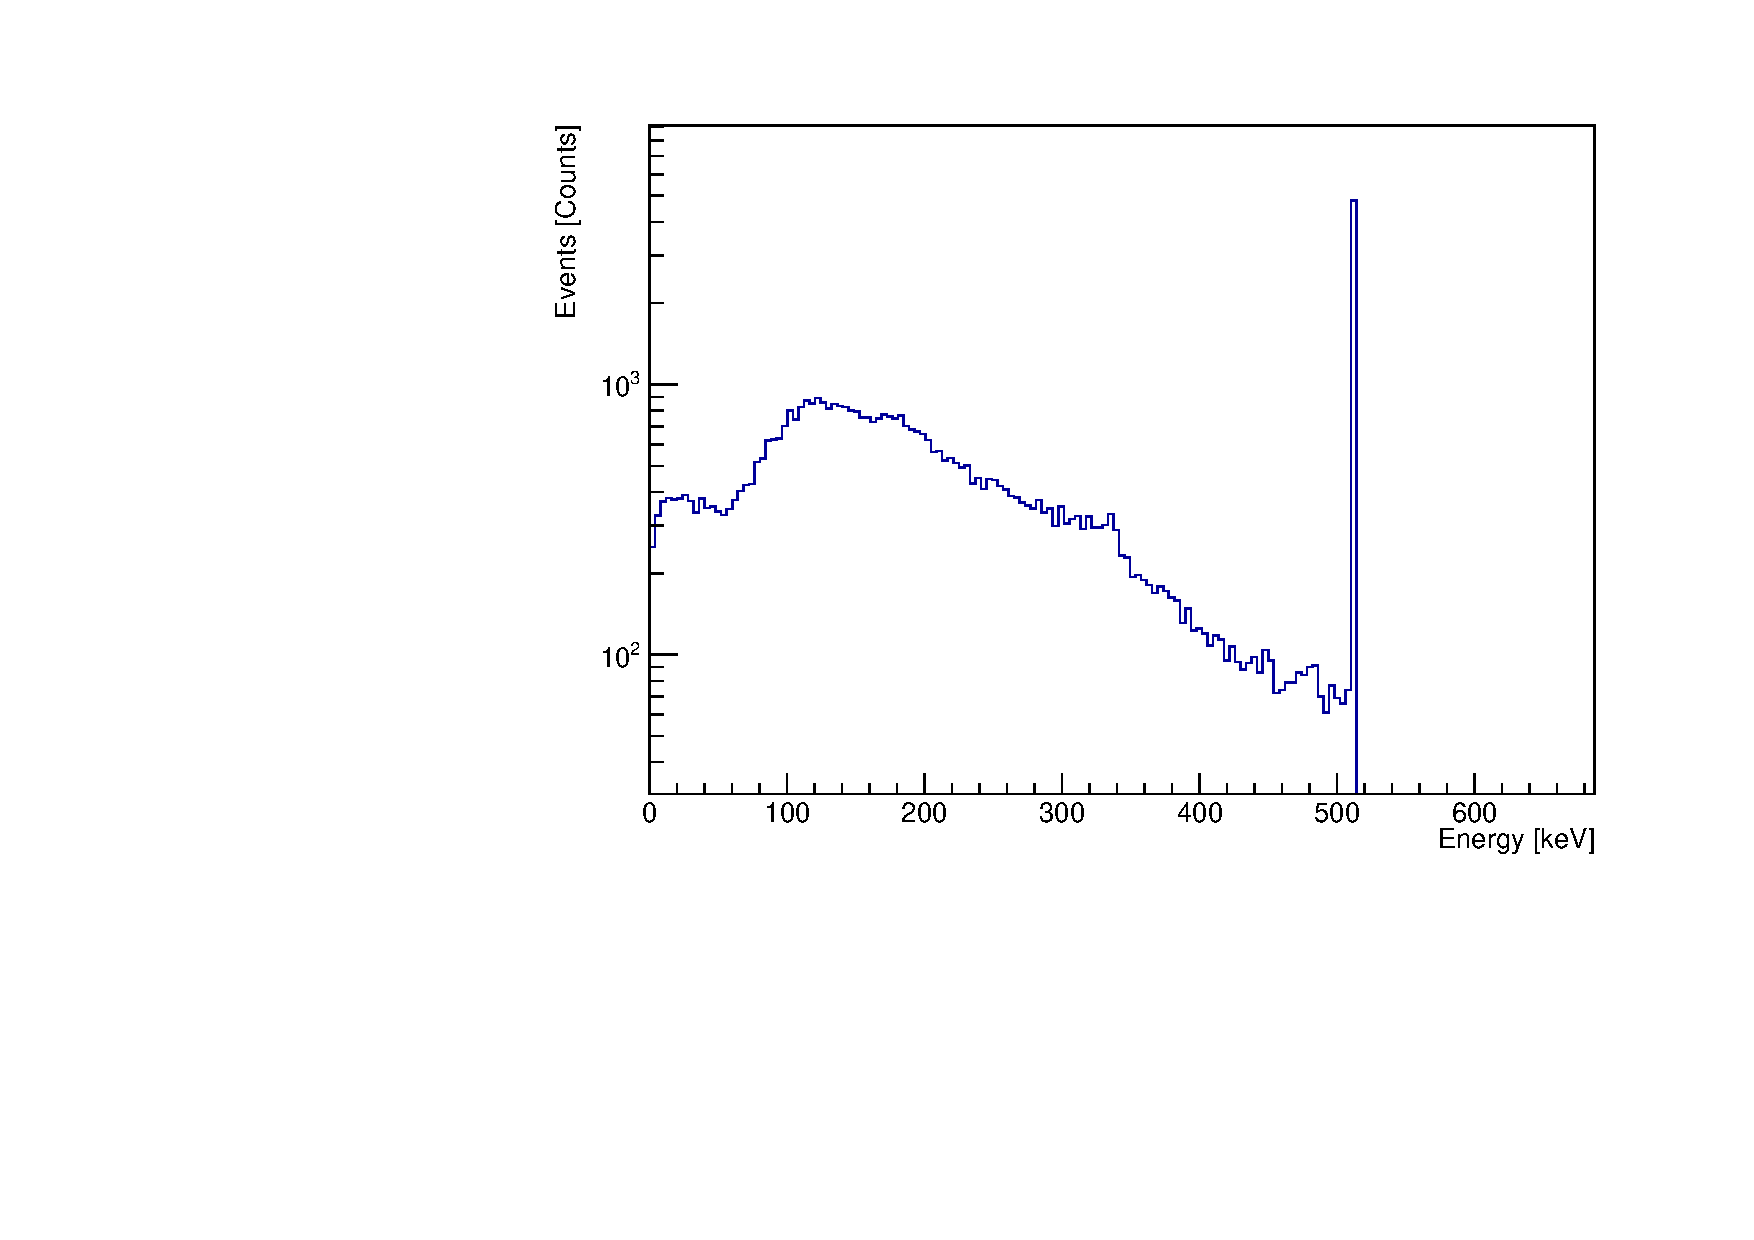
\includegraphics[width=100mm]{./Bilder/MC-514-Phasenraum.pdf}
	\fi%
	\caption{
    Spectrum of the measured rare \Kr events in all of the BEGe detectors of the Monte Carlo simulation.
	}
	\label{fig:PhasenraumMC514}
\end{figure}

Now that the conversion factors of the two types of detectors are determined we can calculate the density of all \Kr decays by applying formula \ref{equ:density}

\begin{equation}
\rho_{dec} = \frac{\mathrm{N}}{p}\times\frac{1}{\epsilon_\gamma V_{sim}}
\label{equ:density}
\end{equation}

where p = 0.434$\%$ is the probability of a \Kr to decay into the 514keV energetically raised \nuc{Rb}{85m}.
For an amount of 27.24\(\pm\)3.87 events to be measured in the BEGe detectors, it can be concluded that a density for the \Kr decay of, whereas for the COAX detectors we get a value of . 
\\


\section{Calculating the Activity}
\label{sec:CalcActiv}

All we need now to calculate the mean activity of \Kr in \PII~ is the measuring time of all detectors.
But this is not as easy as it seems.
Firstly we have the problem that not all detectors were measuring over the curse of \PII~ and that there were time intervals in which no measurement was recorded at all.
This can easily be solved by looking at the effective measuring time of each detector individually.
The effective measuring time of a detector can easily be determined by looking at how many test pule signals have been recorded by it. 
Since the test pulse signals have been set to a frequency of 0.05Hz over the entire \PII~, an effective measurement time can be achieved by determining the number of detected test pulse signals and then multiply it by 20 seconds.
The individual measuring times are therefor given by
\begin{equation*}
    t_\mathrm{i} = \mathrm{N}_{TP}(\mathrm{i}) \times 20\mathrm{s}
\end{equation*}
where i is the index of the respective input channel of each BEGe detector.
\\

The second problem arises from the fact that we calculated the decay density with the assumption that we could merge all detectors of the same kind into a single detector.
But now that we want to look at the measurement time of each individual detector, this assumption does not hold true.
There are now two different workarounds we could take.
\\

In the first method we would rerun our Monte Carlo simulation, this time considering the amount of time each detector was actually measuring.
This would be very inefficient.
\\

The second method works around the merging problem by calculating an average measurement time for all detectors.
With this you could then calculate with the detector block as if all detectors of one kind were such a single detector.
This is very elegant solution because no new computation of a simulation is necessary.
\\

For this average measuring time one has to consider the fact that we also have to apply a weigh on every individual measuring time.
This arises from the fact that every BEGe detector has an individual mass.
As we know, the detector efficiency of a single detector is directly dependent on its mass.
If we want to combine all single detectors into one large detector, we have to consider that heavier detectors contribute more to the measured decay rate than lighter detectors.
It is therefore necessary to weight the measuring time of each detector with its individual mass.
Coincidentally, the multiplication of the individual measuring time of a detector with its mass is also the exposure this  single detector.
This means that to calculate the mean measuring time, we just have to divide the combined exposure of all detectors of the same kind by their combined mass.
\\

No matter what approach you take, you can now determine the mean measuring times using equation \ref{meanmeauringtime}.

\begin{equation*}
    \bar{t} = \frac{\sum_\mathrm{i} t_\mathrm{i} \times m_\mathrm{i}}{\sum_\mathrm{i} m_\mathrm{i}} = 1.592
\label{meanmeauringtime}
\end{equation*}

From this, an average measurement time for the BEGes of  and for the COAX of can be calculated.
With these mean measuring times we can now finally calculate the mean specific activity $\bar{a}$ of \Kr over the curse of all of \PII~ by applying
\begin{equation*}
    \bar{a} = \frac{\rho_{dec} }{\bar{t}} = \frac{\mathrm{N}}{p}\times\frac{1}{\epsilon_\gamma V_{sim}}\times\frac{1}{\bar{t}}
\end{equation*}


With the line count rate analysis we are now finally able to determine an activity of $\bar{a}_{\mathrm{1,BEGe}} = (5.46\pm0.827)\times10^{-4}	\frac{\unit{Bq}}{\unit{l}}$ in the BEGes and a specific activity of $\bar{a}_{\mathrm{1,COAX}} = (4.70\pm0.887)\times10^{-4}	\frac{\unit{Bq}}{\unit{l}}$ in the COAX.
These two values differ only inside their range of uncertainty which is why these results are of good quality.
Of these two value we can now also calculate a mean specific activity $\bar{a}_{1} = (5.08\pm0.857)\times10^{-4}\frac{\unit{Bq}}{\unit{l}}$.
\\

We can now make some comparisons of this value with the WARP and the Darkside experiments.
In the case of the WARP experiment a specific activity of $(160\pm130)\frac{\unit{mBq}}{\unit{l}}$ \label{} was measured for the \Kr.
On the other hand, an specific activity of $(2.8577 \pm 0.18122) \frac{\unit{mBq}}{\unit{l}}$ was measured in the Darkside experiment.
Our determined value of $(0.508\pm0.085)\frac{\unit{mBq}}{\unit{l}}$ is about one order of magnitude smaller than the specific activity in the Darkside and whole three orders of magnitude smaller than the WARP experiment.
From these comparisons we can see that our results seem to verify the first approximations mentioned in the introduction predicting that the \Kr activity seems to be much smaller than in other experiments using liquid argon.
\\

What we can also do now is take the specific activities of the other two experiments and determine how many counts we would have measured if the \Kr had their specific activity.
As simplification we restrict ourselves here to the theoretical values that could be measured in the BEGe detectors. 
How many counts the corresponds activity would induce in the BEGe detectors we can determine with the help of formula \ref{equ:correspondingEvents}.
\begin{equation}
\mathrm{N} = \bar{a} \times p \times \epsilon_\gamma V_{sim} \times \bar{t}
\label{equ:correspondingEvents}
\end{equation}
With the activity and the values determined from the analysis above we can calculate a corresponding amount of about 76152 events for the WARP experiment and 1360 in the Darkside experiment.
In the case of the WARP experiment one could expect with such a high activity that the count rate is also much higher than the 183 events determined from the actual measurement.
Again for the Darkside experiment we calculate a amount of counts about one order of magnitude higher than the here measured events.
From these comparisons we can see that for a much higher specific activity of \Kr to have actually been present a much bigger amount of events should have been counted.
As a graphical representation, the peaks that one would have been able to be seen in the measured spectrum are displayed in figure \ref{fig:WARP} and \ref{fig:Darkside}.
In both diagrams the actually measured spectra are also displayed, even if they are not recognizable as in the case of the WARP peak.
\\

\begin{figure}[t!]
	\centering
	\begin{subfigure}{.5\textwidth}
		\centering
		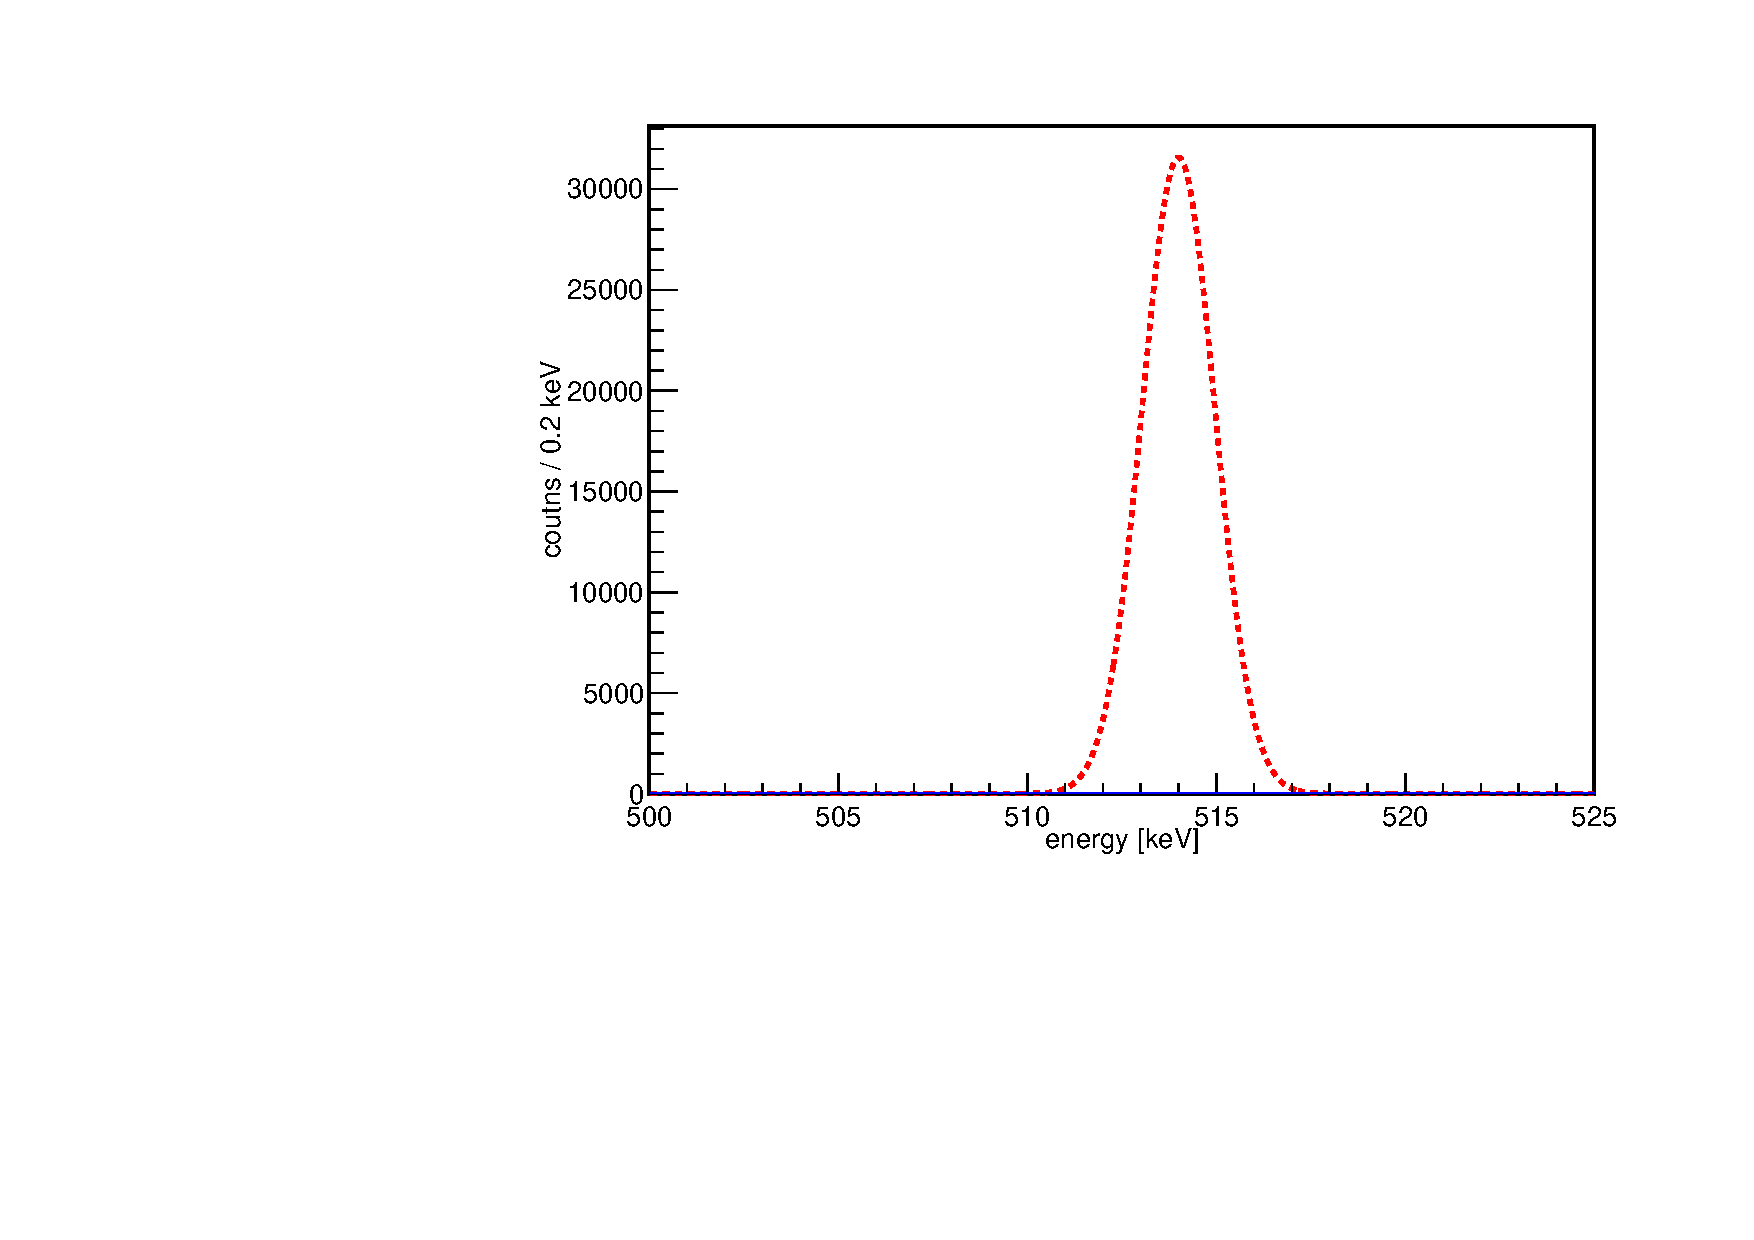
\includegraphics[width=75mm]{./Bilder/WARP.pdf}
		\caption{Cross section from above}
		\label{fig:WARP}
	\end{subfigure}%
	\begin{subfigure}{.5\textwidth}
		\centering
		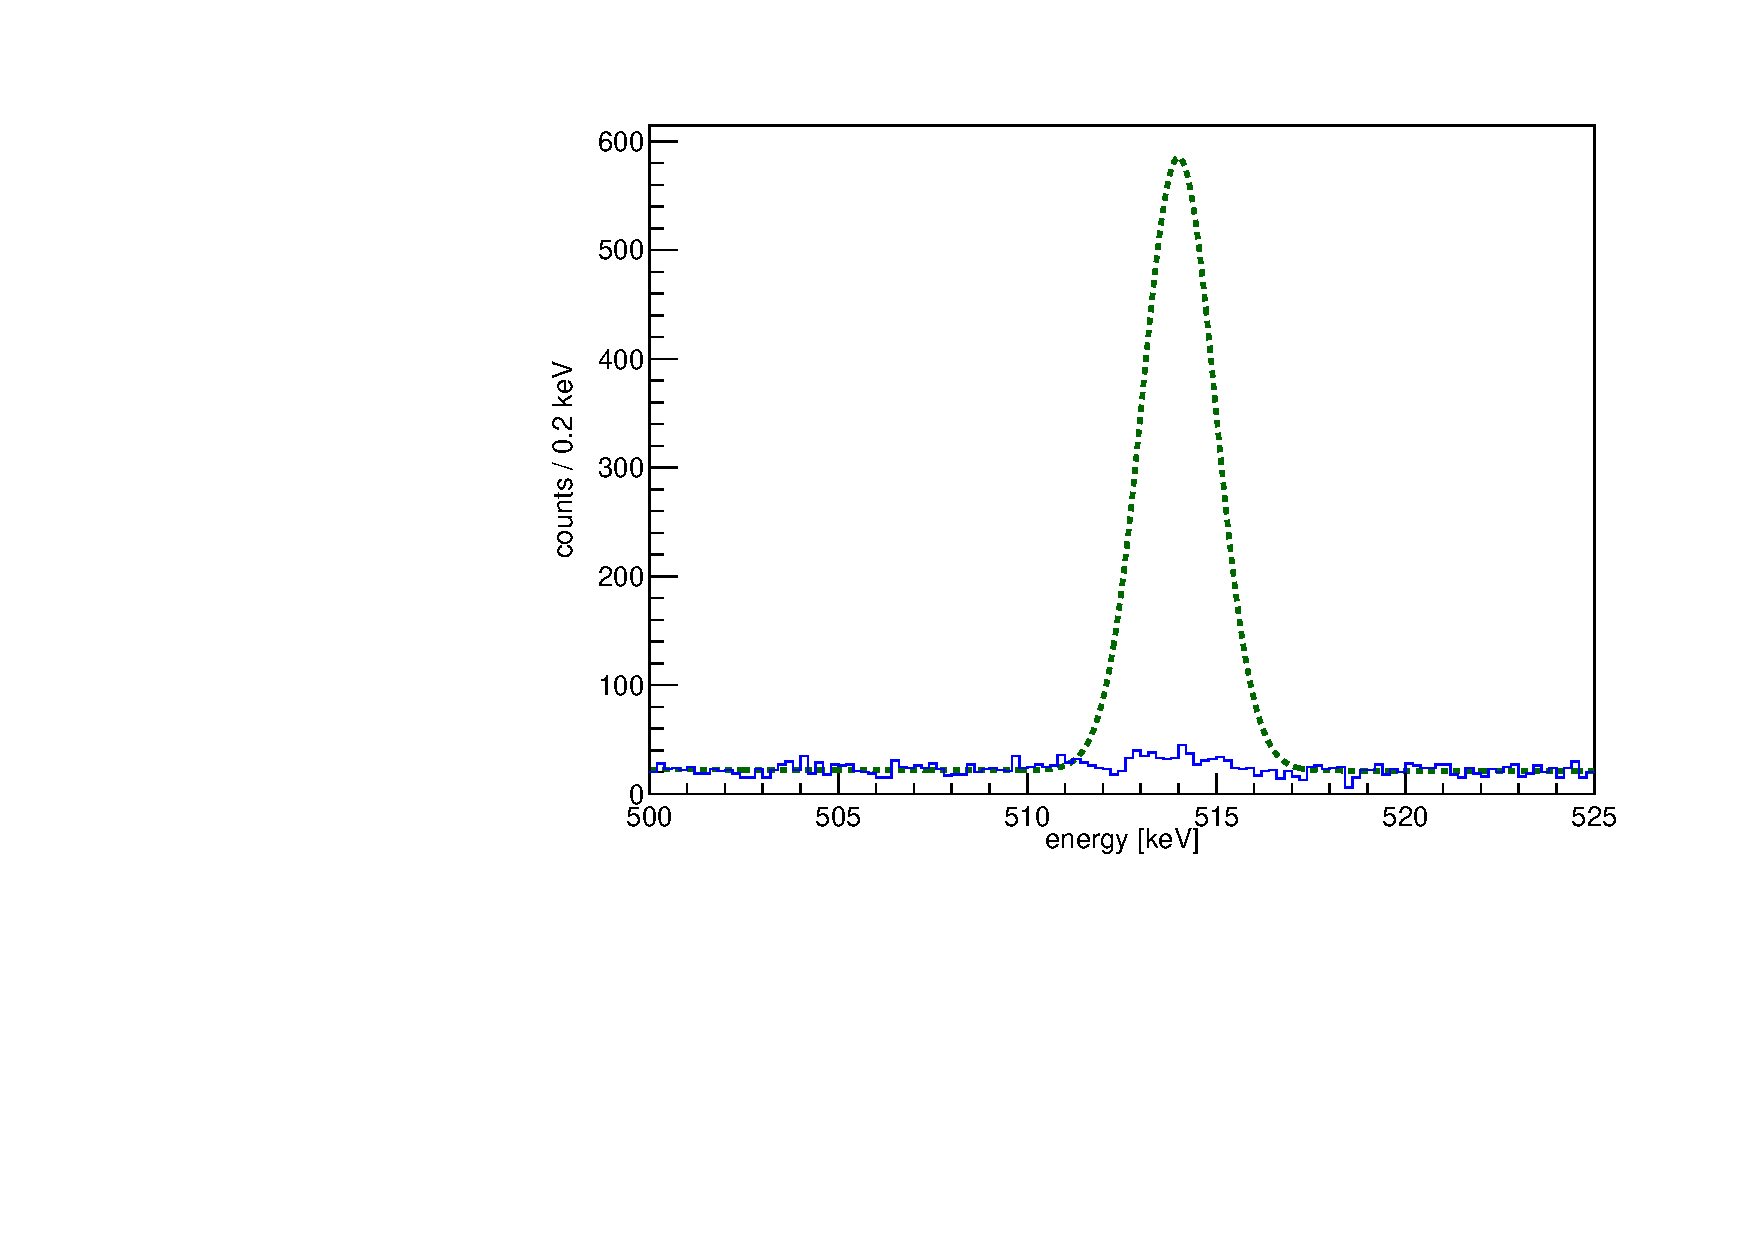
\includegraphics[width=75mm]{./Bilder/Darkside.pdf}
		\caption{Radial cross section}
		\label{fig:Darkside}
	\end{subfigure}
    \\
	\vspace{0.5cm}
    \caption{}
\vspace{0.5cm}
\end{figure}
\\

Now that we have determined a concrete value for the specific activity of \Kr we now come to our second attempt to measure the specific activity as described in the next chapter.
\\  




%	4.70E-04	8,87E-05	Bq/l


% calculate Amplitude of Gauss peak at 514keV and use factor from Monte Carlo Simulation to estimate

% look at phase diagram at range of 500 to 525 keV, use different filters and fit remaining data with Gaussian function
% -> get amplitude
% make a Monte Carlo simulation to estimate actual Kr85 activity in LAr from measured activity in detectors
% -> with amplitude and factors from MC-Simulation one can calculate the specific activity

\chapter{Activity from the Decrease in Rate}
\label{sec:SAfromDecrease}

As described in the beginning of section \ref{sec:AotKr}, the line count analysis method of the rare \Kr decay was expected to be relatively precise.
By following this procedure we were able to determine the activity down to the order of 10$^{-4} \frac{\mathrm{Bq}}{\mathrm{l}}$ with reasonable uncertainty.
We will now concentrate on implementing and discussing the second approach of determining the specific activity by using the change of event rate over time.
Because this method does not rely on any of the values used in the line count rate analysis this approach is truly completely independent of the other method.
Ideally, a positive result from this method would confirm the specific activity determined in the previous chapter. 
\\

But as it was also stated above, the second method is expected to be relatively imprecise.  
This estimation came from the fact that this method relies on a great approximation.
For this method to be applied it is necessary to expect that in the time interval of all of \PII~ only the intensity of the \Kr isotope has a non negligible change in its intensity.
The idea behind this comes from the fact that \Kr has the lowest half life \(T = 10.739\unit{y}\) of all the other residual radioactive isotopes in the liquid argon.
In comparison, other radioactive isotopes that are of interest here are \nuc{Ar}{42} with a half-life of 32.9 y \cite{chen_nuclear_2016}, \nuc{Ar}{39} with 269 y \cite{singh_nuclear_2006} and \nuc{Po}{210} with 138d \cite{kondev_nuclear_2008}. 
\\

\nuc{Po}{210} has a much lower half life than \Kr but the energy of the escaping alpha particle much higher than the mean beta energy of all of the isotopes above.
This is important, because over the course of this chapter we will at some point begin to only consider those events in our analysis that deposited an energy between 200 and 400 keV.   
This means even though \nuc{Po}{210} has a much lower half life it would not create much of a change in event rate due to its very low probably to release an alpha particle in this energy range.
\\

On the other hand, the two different types of argon isotopes have both a mean beta energy close to \Kr's 251.59 keV.
Their change in event rate should therefor be measurable by our approach.
The change in activity of \nuc{Ar}{39} can be neglected because its half life way to big.
\nuc{Ar}{42} on the other hand has a half life that is in the same order of magnitude as \Kr.
But its specific activity has already been determined to be about $148\mui Bq/l$ \cite{becerici_schmidt_results_2014} which is about factor 3.5 smaller than the expected \Kr specific activity.
Whether or not we have to consider the influence of this isotope will be discussed later in this theses.
For now we will apply the simplification that its change will be small compared to \Kr.
\\

All other radioactive isotopes that are residual in the liquid argon have either a much longer half life than \nuc{Ar}{42}, their mean beta energy is much higher than 400keV or their specific activity is too small too small to measure any kind of change over time.
It is therefor approximated that all change in intensity should only originate from the \Kr decay.
But even if the activity determined by this method is not expected to have a much of a value for us, it can still be used as a crosscheck for the other activity determined above.
\\

We have now shown that this approach can be applied here and that it actually serves a purpose.
Now it has to be discussed how exactly the specific activity can be determined by changing the intensity.
To measure the change in rate every measured event will have to be drawn over time and through it an exponential fit applied.
The amplitude of the resulting exponential function represents an event rate with which events in the investigated energy range occur.
\\

To calculate the specific activity of \Kr with this value one again has to use a Monte Carlo simulation to calculate a fitting conversion factor. 
We cannot use the same simulation from the first method because in this case we actually have to simulate \Kr events, not only the emission of 514keV photons as it was done in the prior chapter.
That is why another Monte Carlo simulation has to be carried out.
With it a new conversion factor can be determined to calculate the \Kr decay density necessary to create the measured event activity.
\\

Finally the specific activity can be calculated from these two values.
It is important to note that this approach determines the specific activity of \Kr at the start of \PII~ while the first method calculates the mean specific activity over all of \PII.
To compare those two results, in the end a mean specific activity of the second method has to be determined.
The following sections will focus on the concrete implementation of this method and the values determined by them.
\\

\section{Event Rate}
\label{sec:EventAct}

\begin{figure}[t!]
	\centering
	\begin{subfigure}{.5\textwidth}
		\centering
		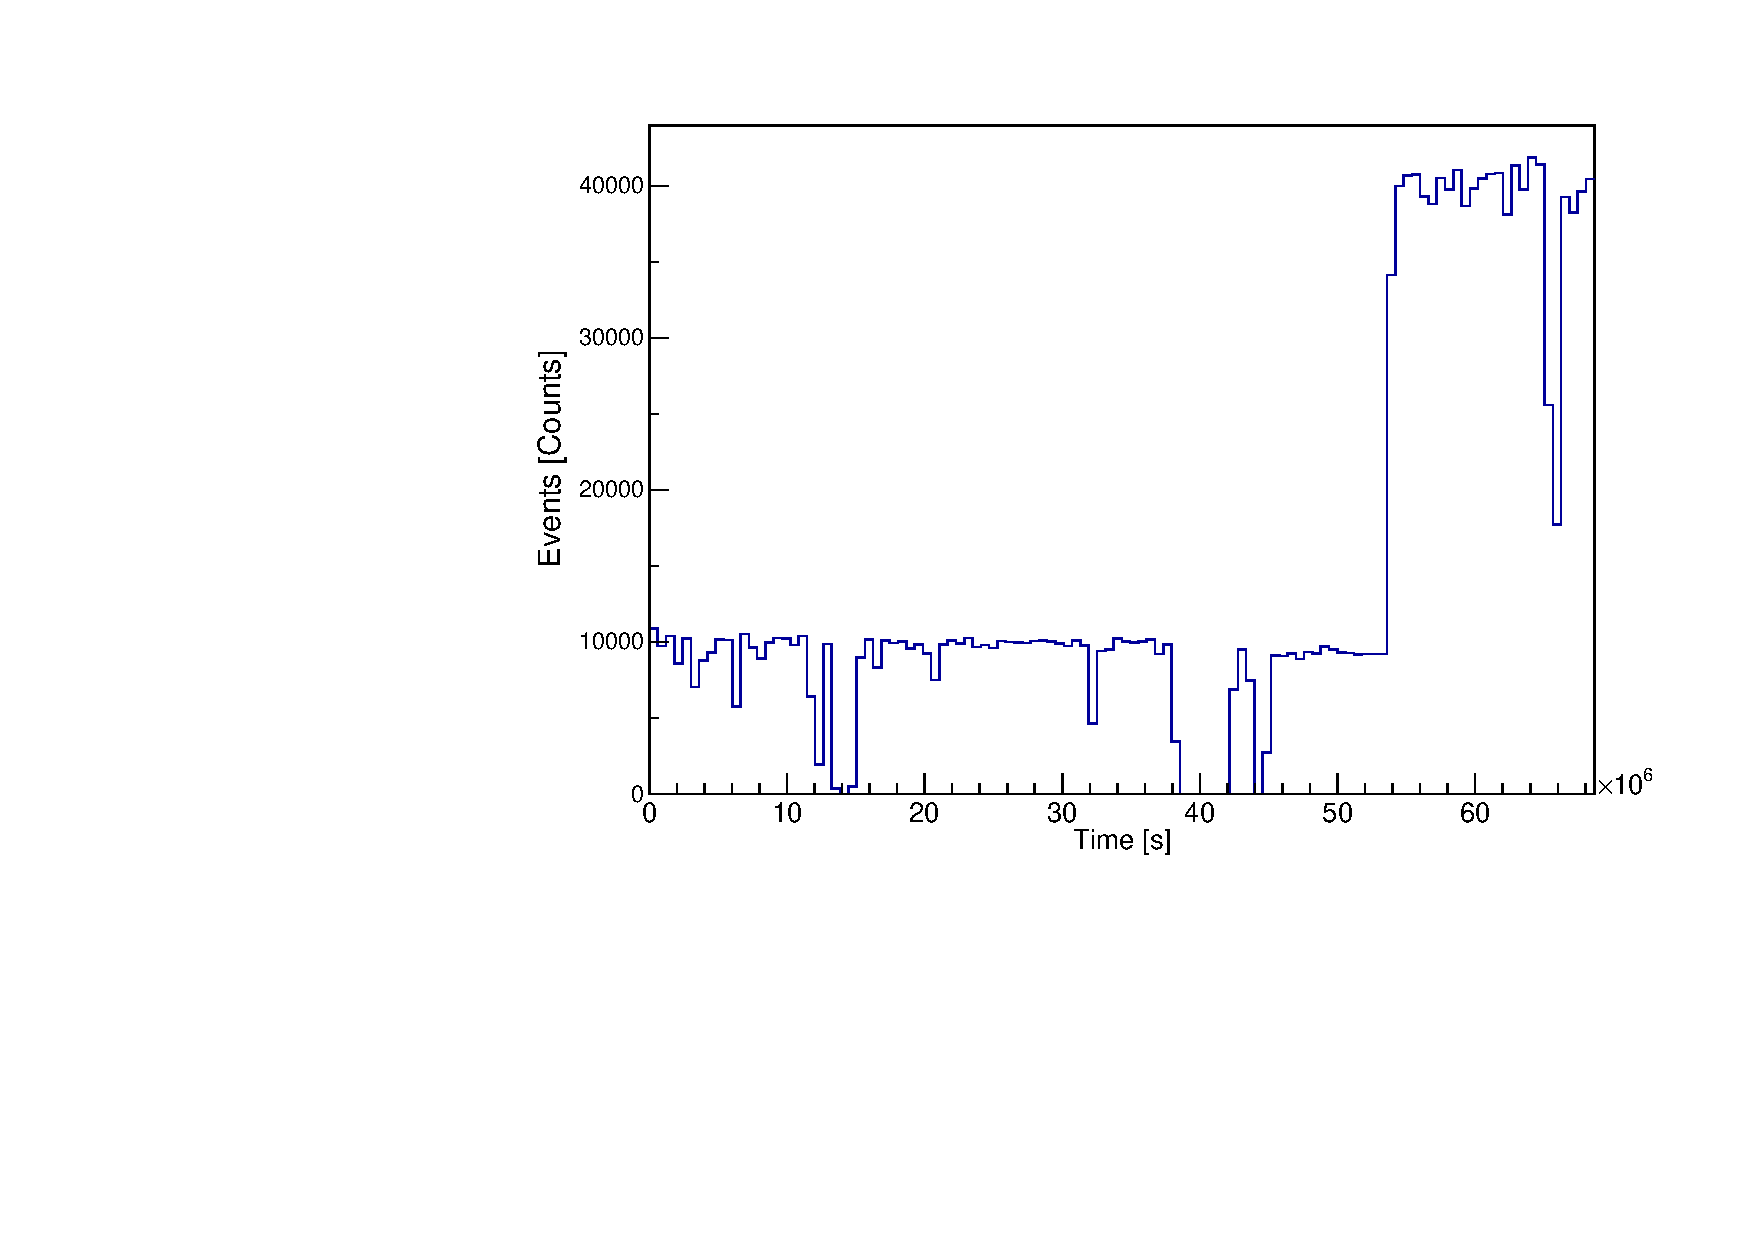
\includegraphics[width=\textwidth]{./Bilder/ZeitverlaufALLE.pdf}
		\caption{every event}
		\label{fig:ZeitAll}
	\end{subfigure}%
	\begin{subfigure}{.5\textwidth}
		\centering
		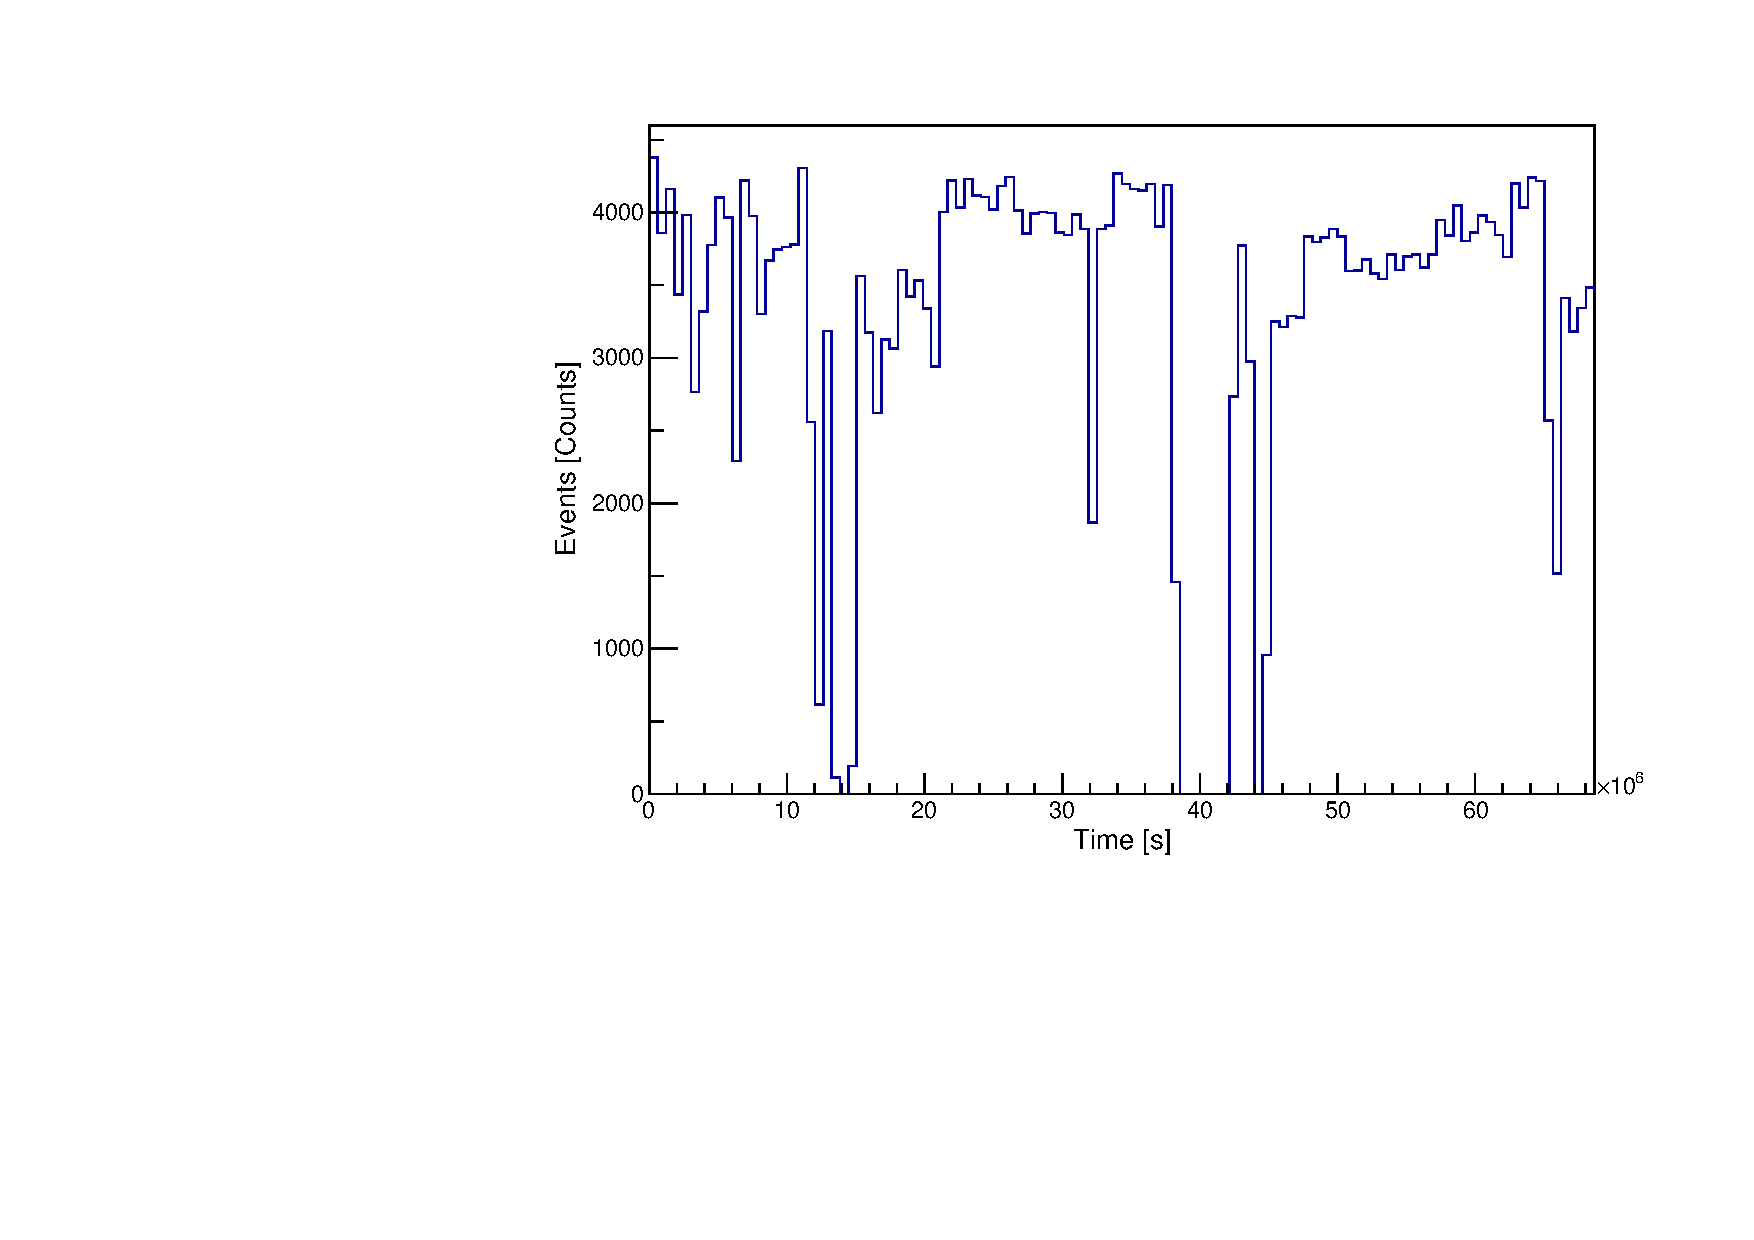
\includegraphics[width=\textwidth]{./Bilder/ZeitverlaufLimits.pdf}
		\caption{only energies between 200 and 400keV}
		\label{fig:ZeitLimits}
	\end{subfigure}
    \\
    \caption{Change of Intensity with time. In both figures are the amount of events measured in one week plotted over the whole time of \PII. In figure (a) no filters were imposed onto the displayed events while in (b) only those events are shown that have an energy between 200 and 400 keV. One can see that further precautions must be taken before an exponential decrease can be determined. }
\end{figure}

To determine the event rate one has to plot the amount of measured events over time in an event histogram with a suitable binning (see figure \ref{fig:ZeitAll}).
In this case a binning of one week per bin was chosen which results in about 114 bins for the 2.17 years of \PII.
As with the line count rate analysis, here we used only these events in the \ref{fig:ZeitAll} histogram where the Muon veto and the detector anticoincidence veto were not triggered.
When looking at the histogram for the first time two things jump into your eye.
Firtsly, there seems to be a great jump in the amount of events measured in the second half of \PII.
And secondly, there are times in which the amount of events measured drop to zero.
These two discontinuous changes to our expected outcome of an exponential decrease make it impossible for us to lay an exponential fit function throug the graph.
We therefor have to find a way to suppress them.
But for this to be done we first have to investigate where these discontinuities originate from.
\\

Firstly, we discuss the big jump in number of events measured.
This jump originates from the change of the lowering of the energy threshold on the 12.10.2017.
This reduction of the lower threshold dramatically increased the number of events measured.
Due to every detector having different characteristics, the limit was set for each detector individually.
Before the lowering the highest limit was set at about 140keV for the BEGes and at 185 for the COAX.
After the lowering all event with an energy of at least about 15keV could be recorded by all detectors.
For a more graphical representation, see the beginning of the spectra in figure \ref{fig:before} for all events measured before and figure \ref{fig:after} for all events after the lowering of the limit. 
This means that from the 12.10.2017 on a much higher event rate was measured just because more event were actually recored.
To work around this continuity problem all we have to do is limit our event used for the analysis to those that have a minimal energy of 200keV. 
While we are already at it we can also set up an upper limit on the energy.
Its purpose is to suppress events caused by isotopes with a higher Q-value energy than \Kr.
Even though they should only create a constant background, but their presence make a change in intensity harder to identify.
We therefor chose the upper limit to be at 400keV.
Theoretically the endpoint energy of \Kr is at 687keV, but the count rate towards the endpoint is that low that we would basically only include more constant background by setting the upper limit higher.
A new plot including only events between the energy limits of 200 and 400keV can be seen in figure \ref{fig:ZeitLimits}.
\\
\begin{figure}[t!]
	\centering
	\begin{subfigure}{.5\textwidth}
		\centering
		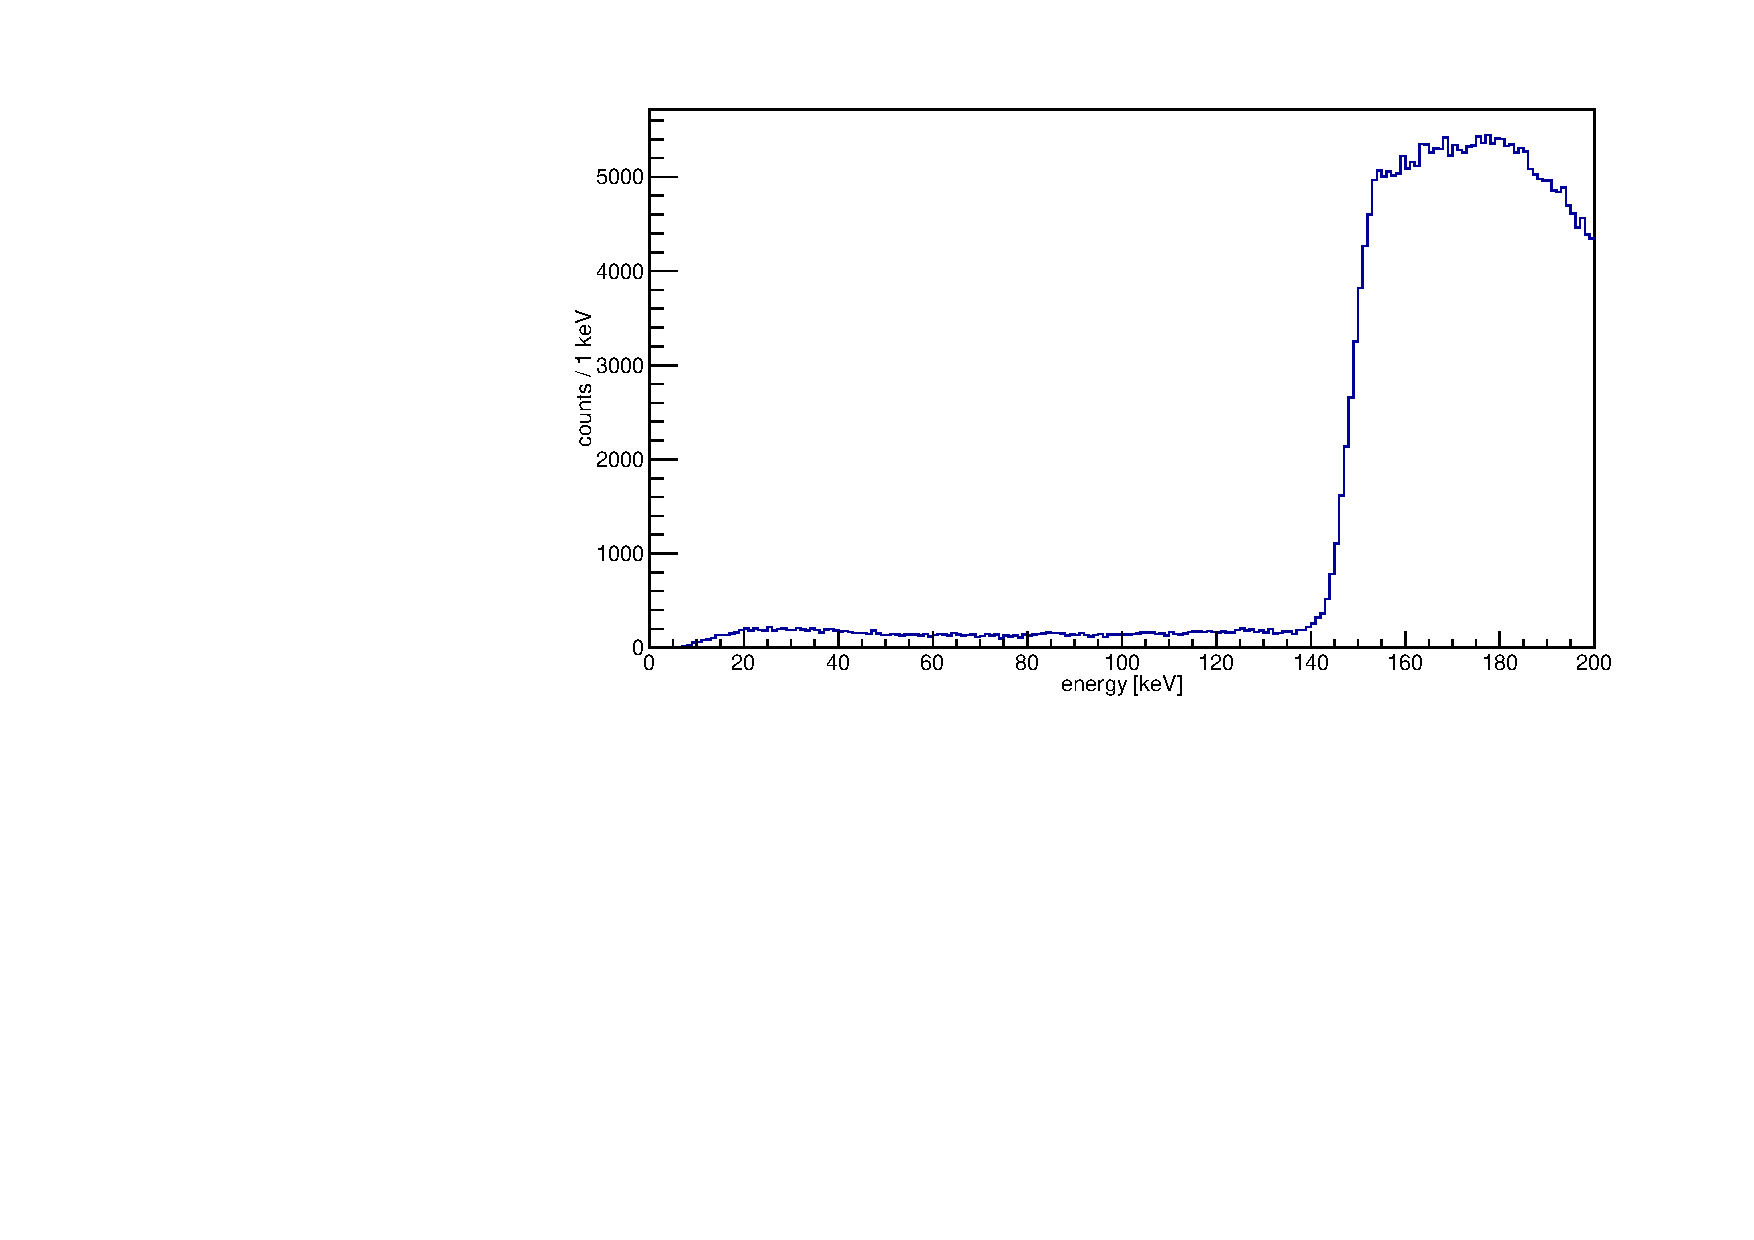
\includegraphics[width=\textwidth]{./Bilder/beforeTheFall.pdf}
		\caption{before}
		\label{fig:before}
	\end{subfigure}%
	\begin{subfigure}{.5\textwidth}
		\centering
		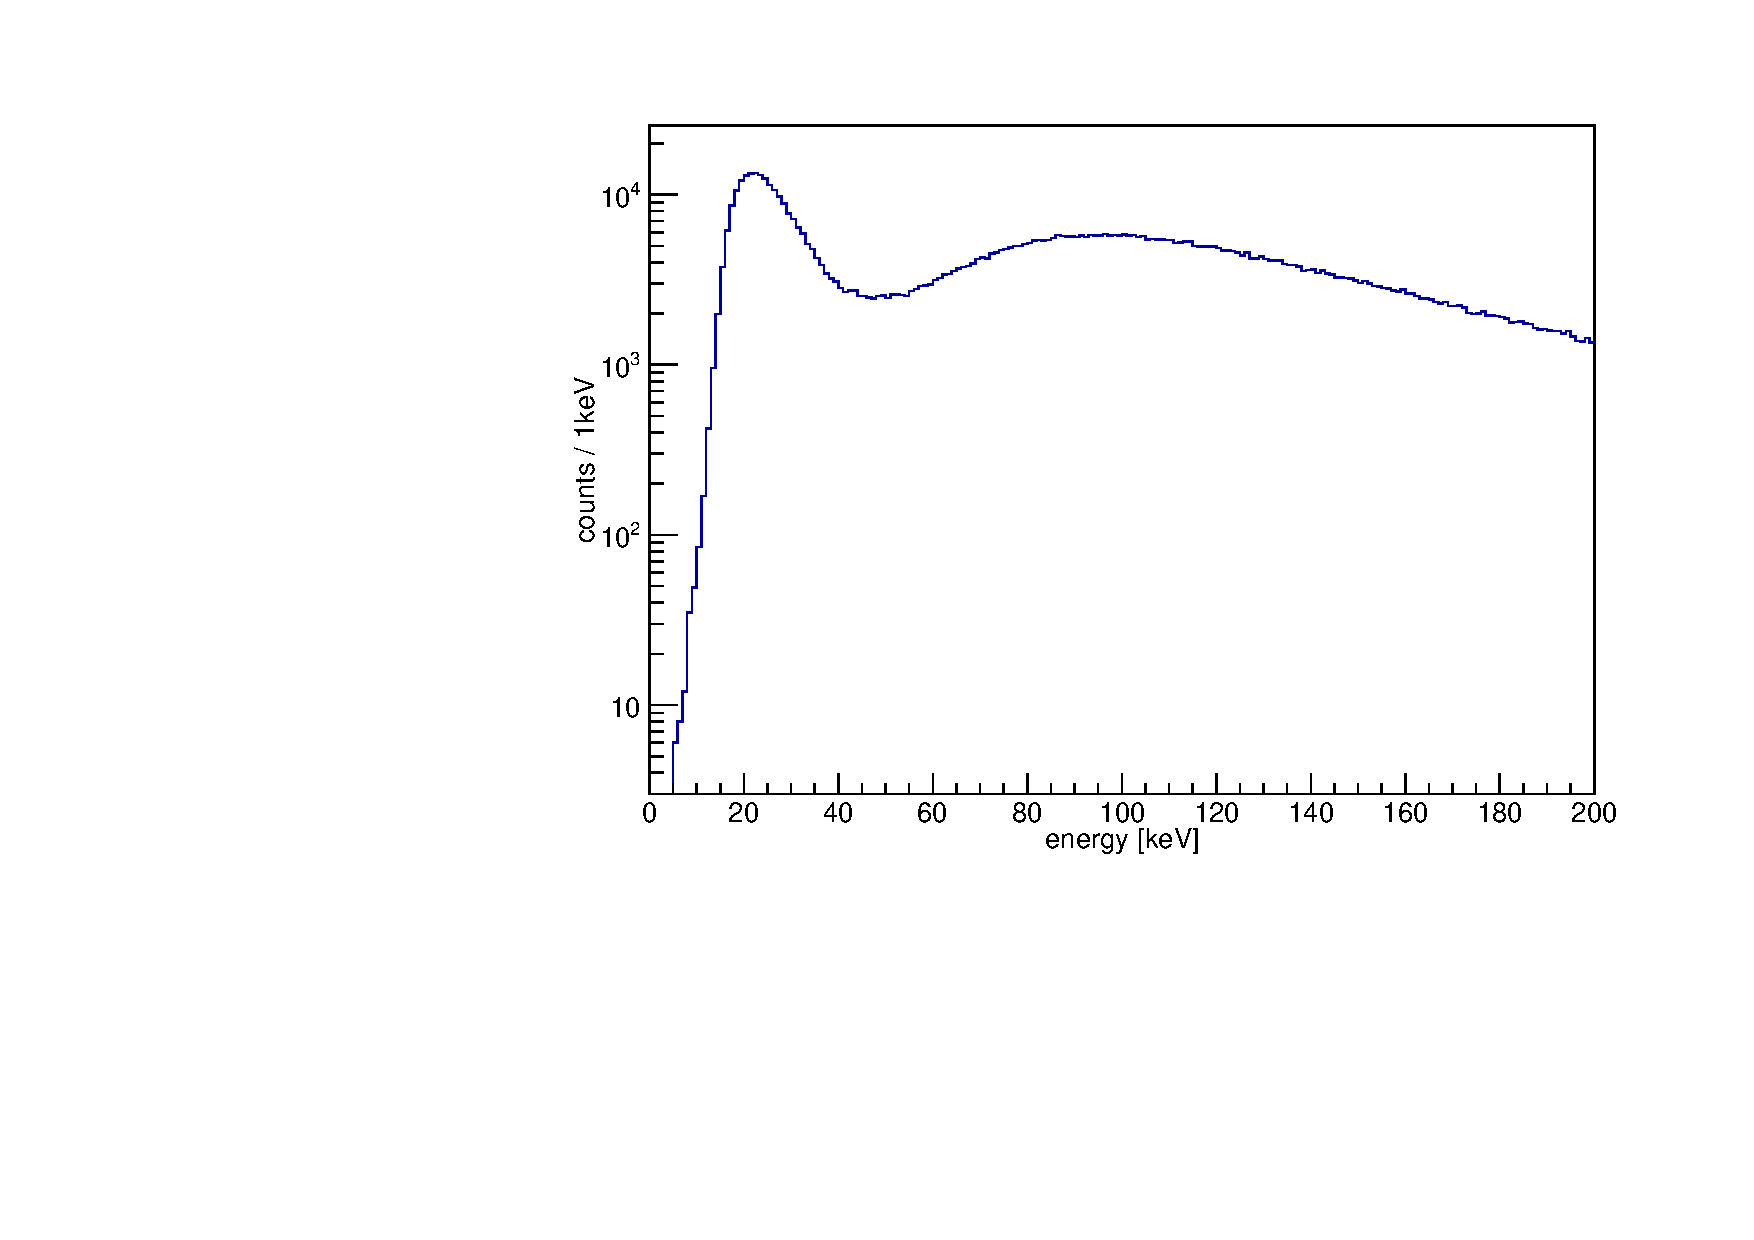
\includegraphics[width=\textwidth]{./Bilder/afterTheFall.pdf}
		\caption{after}
		\label{fig:after}
	\end{subfigure}
	\\
	\vspace{0.5cm}
	\caption{ }
	\vspace{0.5cm}
\end{figure}

The second discontinuous behavior originates from the same problem that we faced in the line count rate analysis.
Not all detectors were on all of the time and there were also time intervals in which no signal at all was recorded.
Due to the fact that some of the detectors were turned on or off over the time of \PII~ will result in discontinuous changes in the event rate because more or fewer events were able to be measured.
But this can easily be solved by only considering those events measured in a detector that was always turned on.
Which detector was always on over all of \PII~ can be seen in figure \ref in the appendix.
On the other hand due to there being time intervals in which no events were recorded the event rate drops discontinuous to zero there.
In section \ref{sec:CalcActiv} we solved this problem by calculating an effective measuring time for each detectors.
Here, however, we are not interested in an average measurement time over the entire \PII.
In this method we must find a way to weigh each individual bin of the event histogram with the corresponding effective measurement time of that bin.
This is where the test pulse signal comes in handy.
It is a clear indication of when exactly data was actually recorded.
This means that similar to the first method we can now determine effective measuring times of each time interval of the bins.
These mean measuring times can easily be calculated by plotting the test pulse signals in an histogram with the same binning as the event histogram and dividing each of these bins with the frequency of the test pulse of $f_\mathrm{TP} = 0.05\unit{Hz}$ (see figure \ref{fig:effectiveMeasuringTimes}).
The contents of these bins in the test pulse histogram correspond now to the respective measuring time in the binning intervals. 
\\

By dividing all bins of the event histogram by the corresponding bins in the test pulse histogram, you would get a new histogram showing the change of events measured in the time intervals of the bins (see figure \ref{fig:ChangeInEventRate}).
Or in other words, this new histogram shows us the event rate per week over all of \PII.
\\
\begin{figure}[t!]
	\centering
	\begin{minipage}{.5\textwidth}
		\centering
		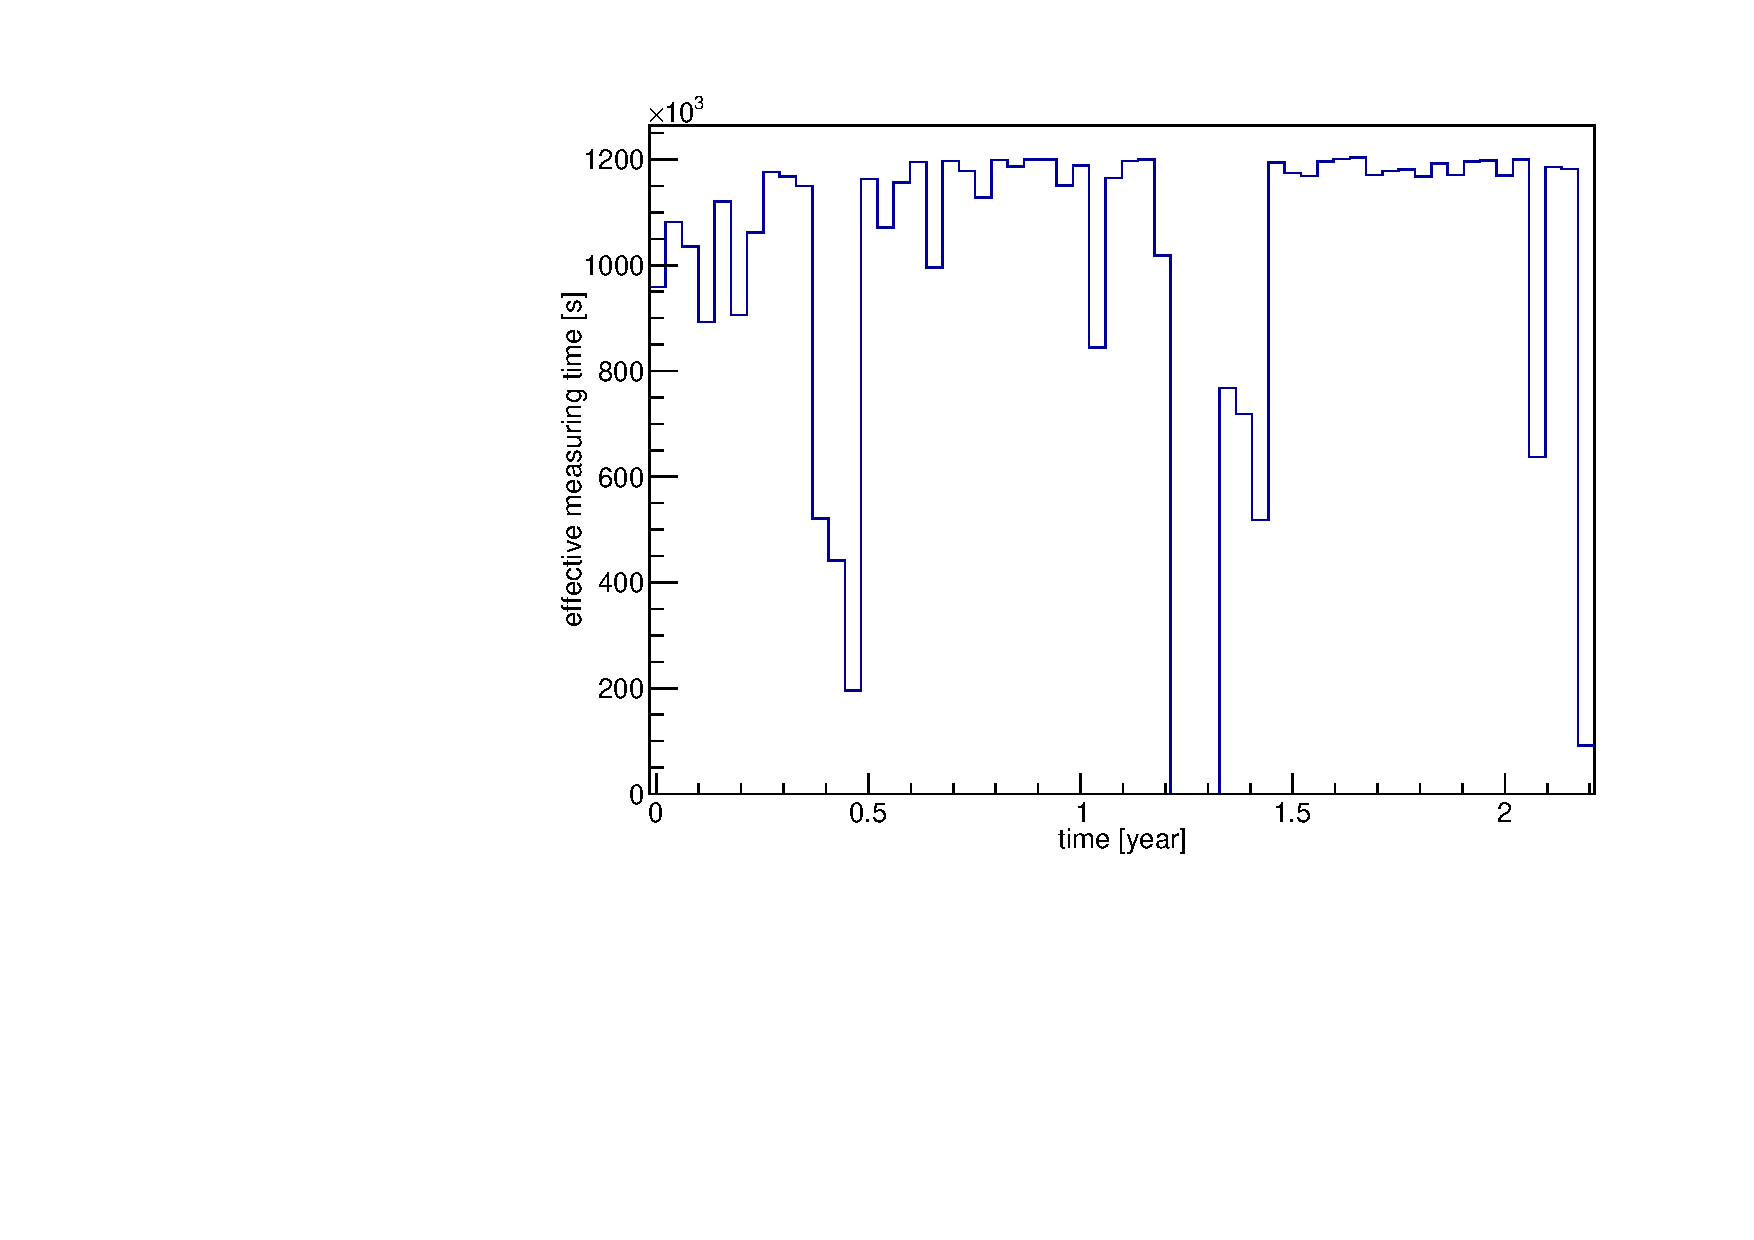
\includegraphics[width=\textwidth]{./Bilder/testpuler.pdf}
		\caption{effective measuring times}
		\label{fig:effectiveMeasuringTimes}
	\end{minipage}%
	\begin{minipage}{.5\textwidth}
		\centering
		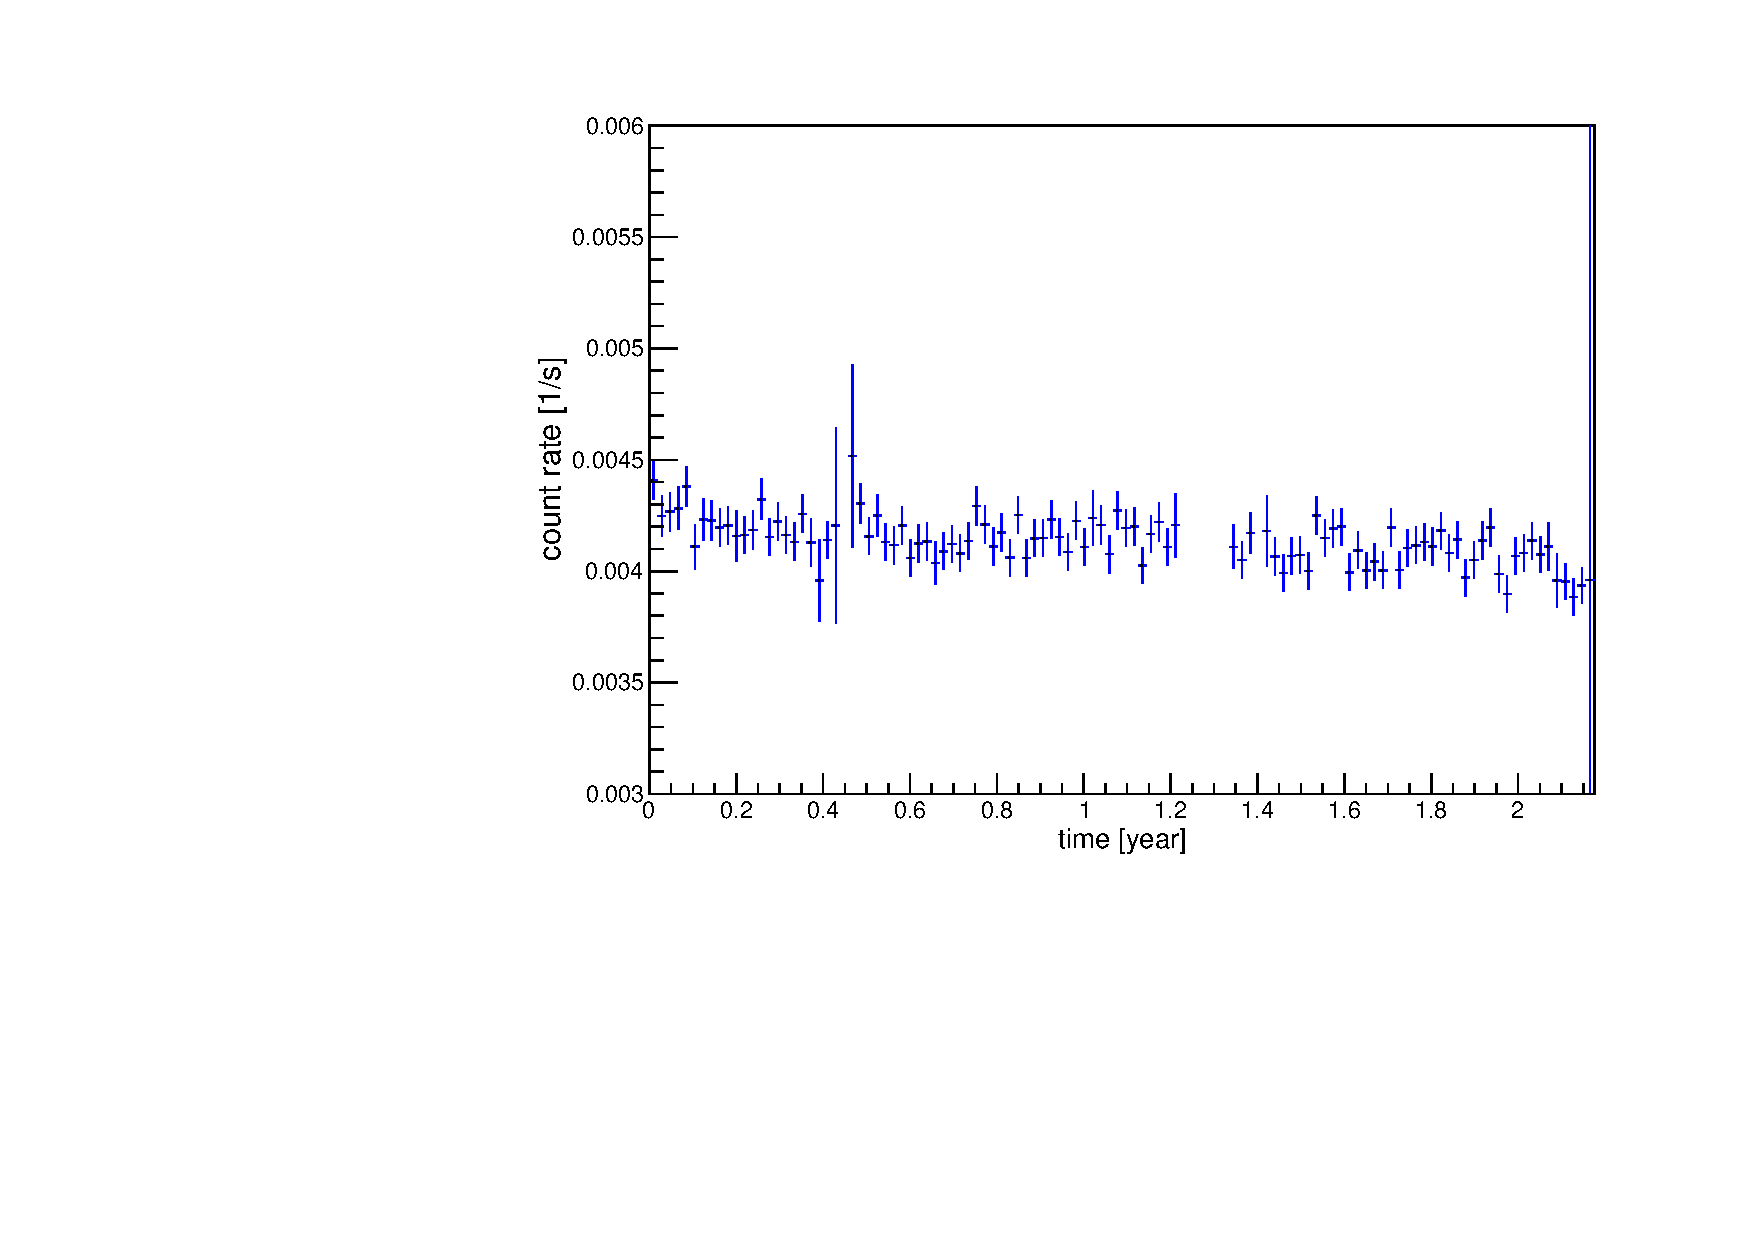
\includegraphics[width=\textwidth]{./Bilder/eventRate.pdf}
		\caption{after}
		\label{fig:ChangeInEventRate}
	\end{minipage}
	\\
\end{figure}

From this graph we now want to determine the exponential change in the event rate by applying an exponential fit function.
The exact fit function used is
\begin{equation}
\mathrm{f}(x) = \mathrm{A}\times\exp\left(-\frac{\log(2)}{\mathrm{B}} x \right) + \mathrm{C}
\label{equ:FitFilters}
\end{equation}
In this is A corresponding to the measured \Kr event rate of the decreasing function, B the half life of the decrease and C the constant event background rate.
Due to us exacting only \Kr to change over time we can already fix fit-parameter B to \(10.739\unit{y}\) which is the half life of \Kr and leaving the other two parameter relatively free.
From the resulting fit function (seen figure \ref{fig:ChangeInEventRateFit}) we get the fit parameters as seen in table \ref{tab:FitParZeit}.
The only parameter we need for our analysis is parameter \(\mathrm{A} = R_{\mathrm{count}} = \) being the \Kr event rate meaning that !!!!! events caused by \Kr decays could be measured every second.
Now that we have the \Kr event rate all we need now to determine the specific activity is the conversion factor from the measured events to the necessary \Kr decays in the liquid argon to cause this \Kr event rate.
As described above we need a new Monte Carlo simulation for that.
What this simulation actually simulates and how we determine the conversion factor from it is the topic of the following section.


\begin{table}[t!]
	\centering
	\begin{tabular}{|l|r|}
		\hline
		Name	& Value  \\ 
		\hline
		A  &	(17.844639 \(\pm\)	3.179471)\\	
		\hline
		B  &	(513.838989 \(\pm\)	0.665171)\\	
		\hline
		C  &	(0.828315 \(\pm\)	1.377836)\\
		\hline
	\end{tabular}
	\caption{Fit parameters of fit function \ref{equ:FitNoFilters} applied on the spectra of the respective detectors.}
    \label{tab:FitParZeit}
\end{table}

\begin{figure}[t!]
	\centering
	\ifmakefigures%
	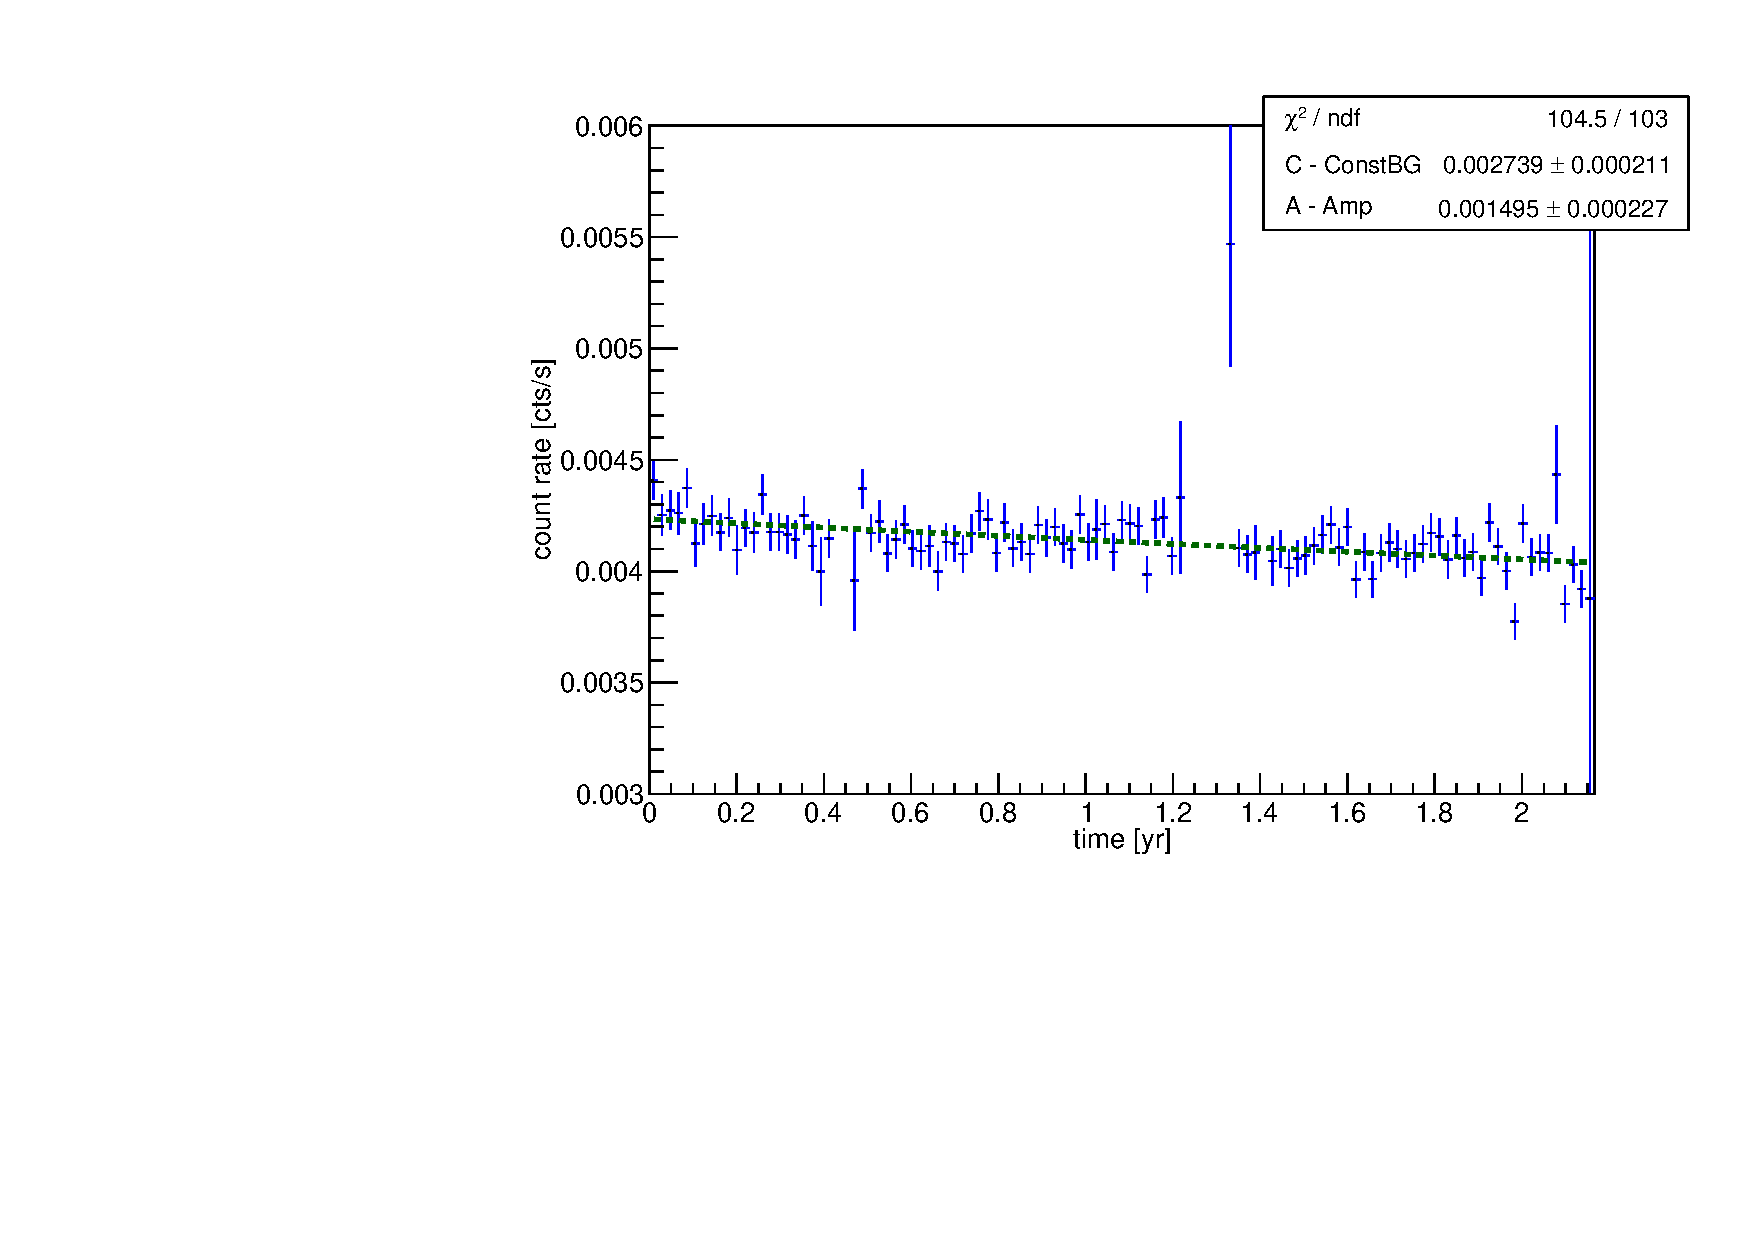
\includegraphics[width=100mm]{./Bilder/eventRateFit.pdf}
	\fi%
	\caption{effective measuring times}
	\label{fig:ChangeInEventRateFit}
\end{figure}%
\begin{figure}[t!]
	\centering
	\begin{minipage}{.5\textwidth}
		\centering
		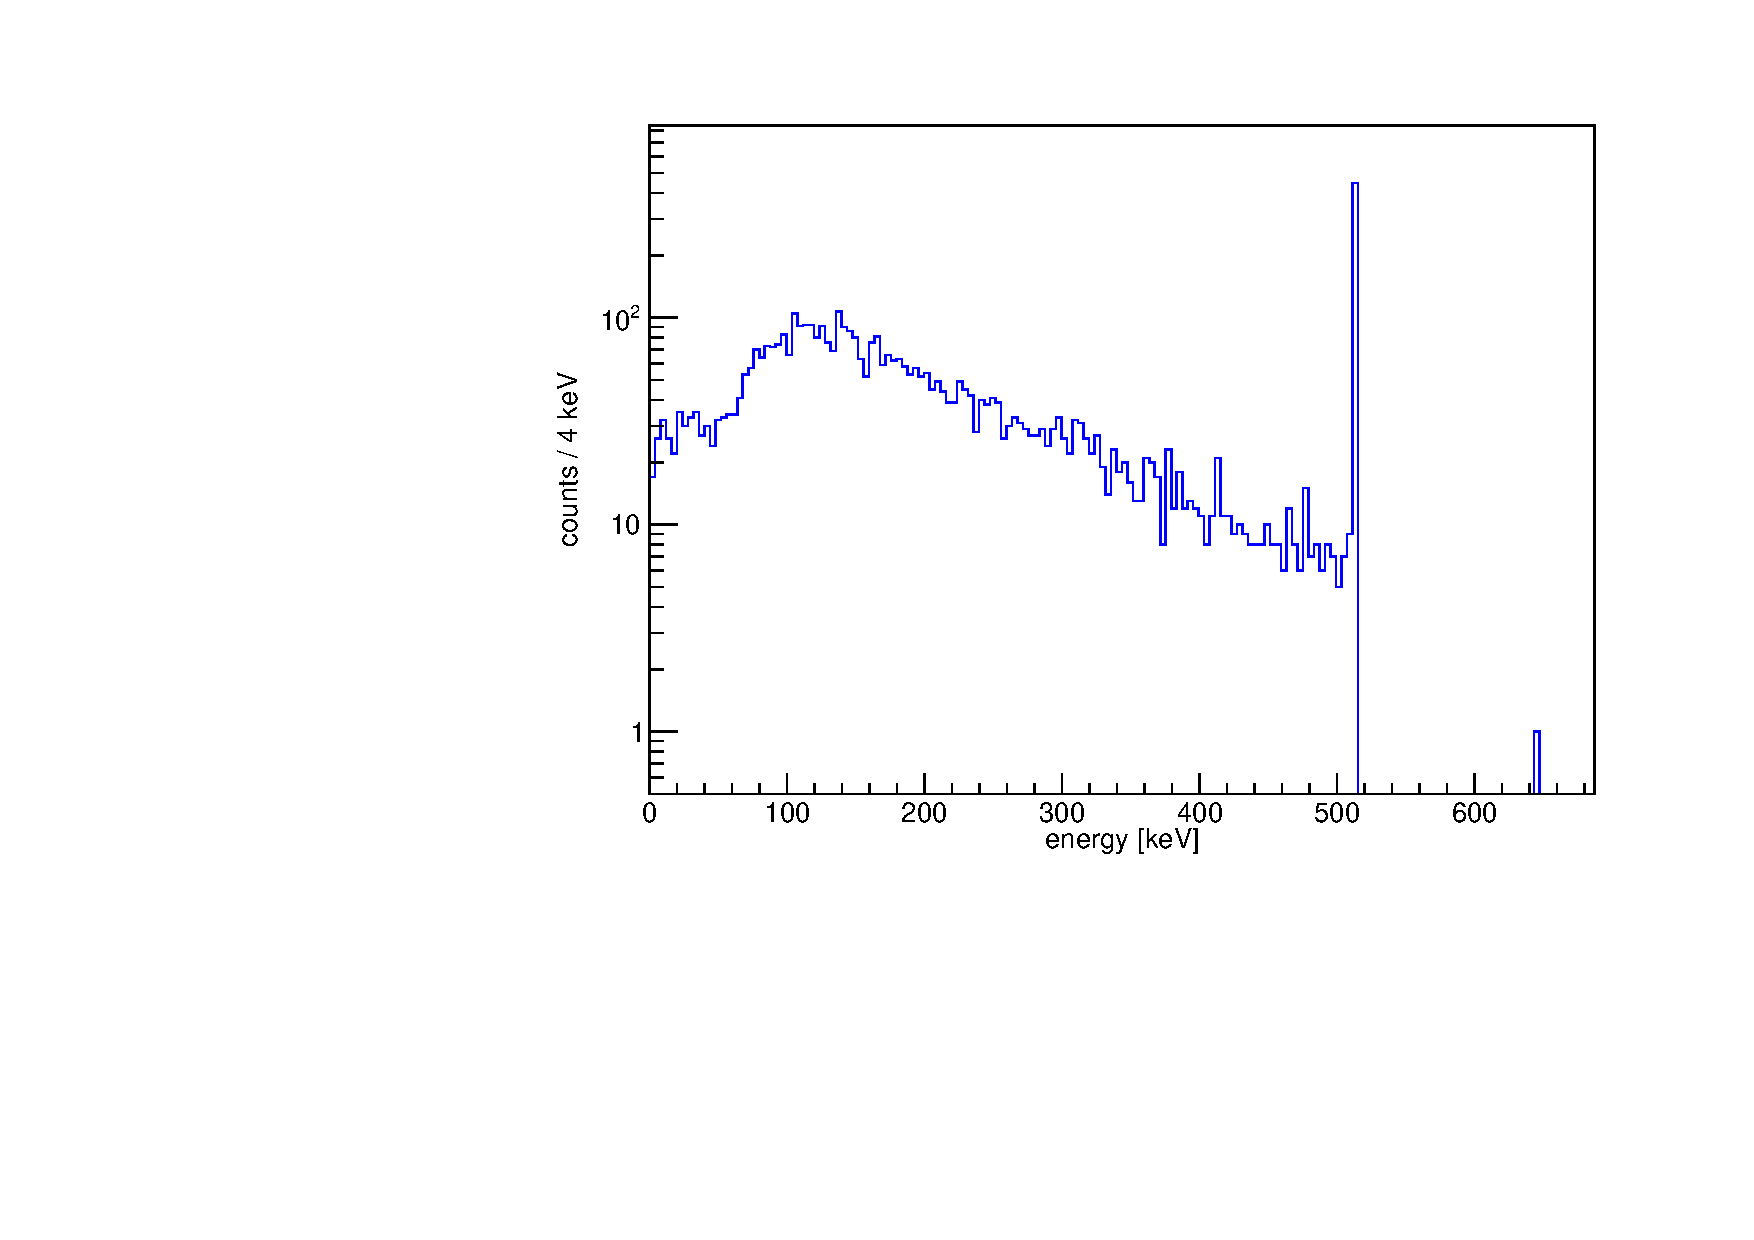
\includegraphics[width=\textwidth]{./Bilder/Sim1Phasenraum.pdf}
		\caption{after}
		\label{fig:Sim1Spektrum}
	\end{minipage}%
	\begin{minipage}{.5\textwidth}
		\centering
		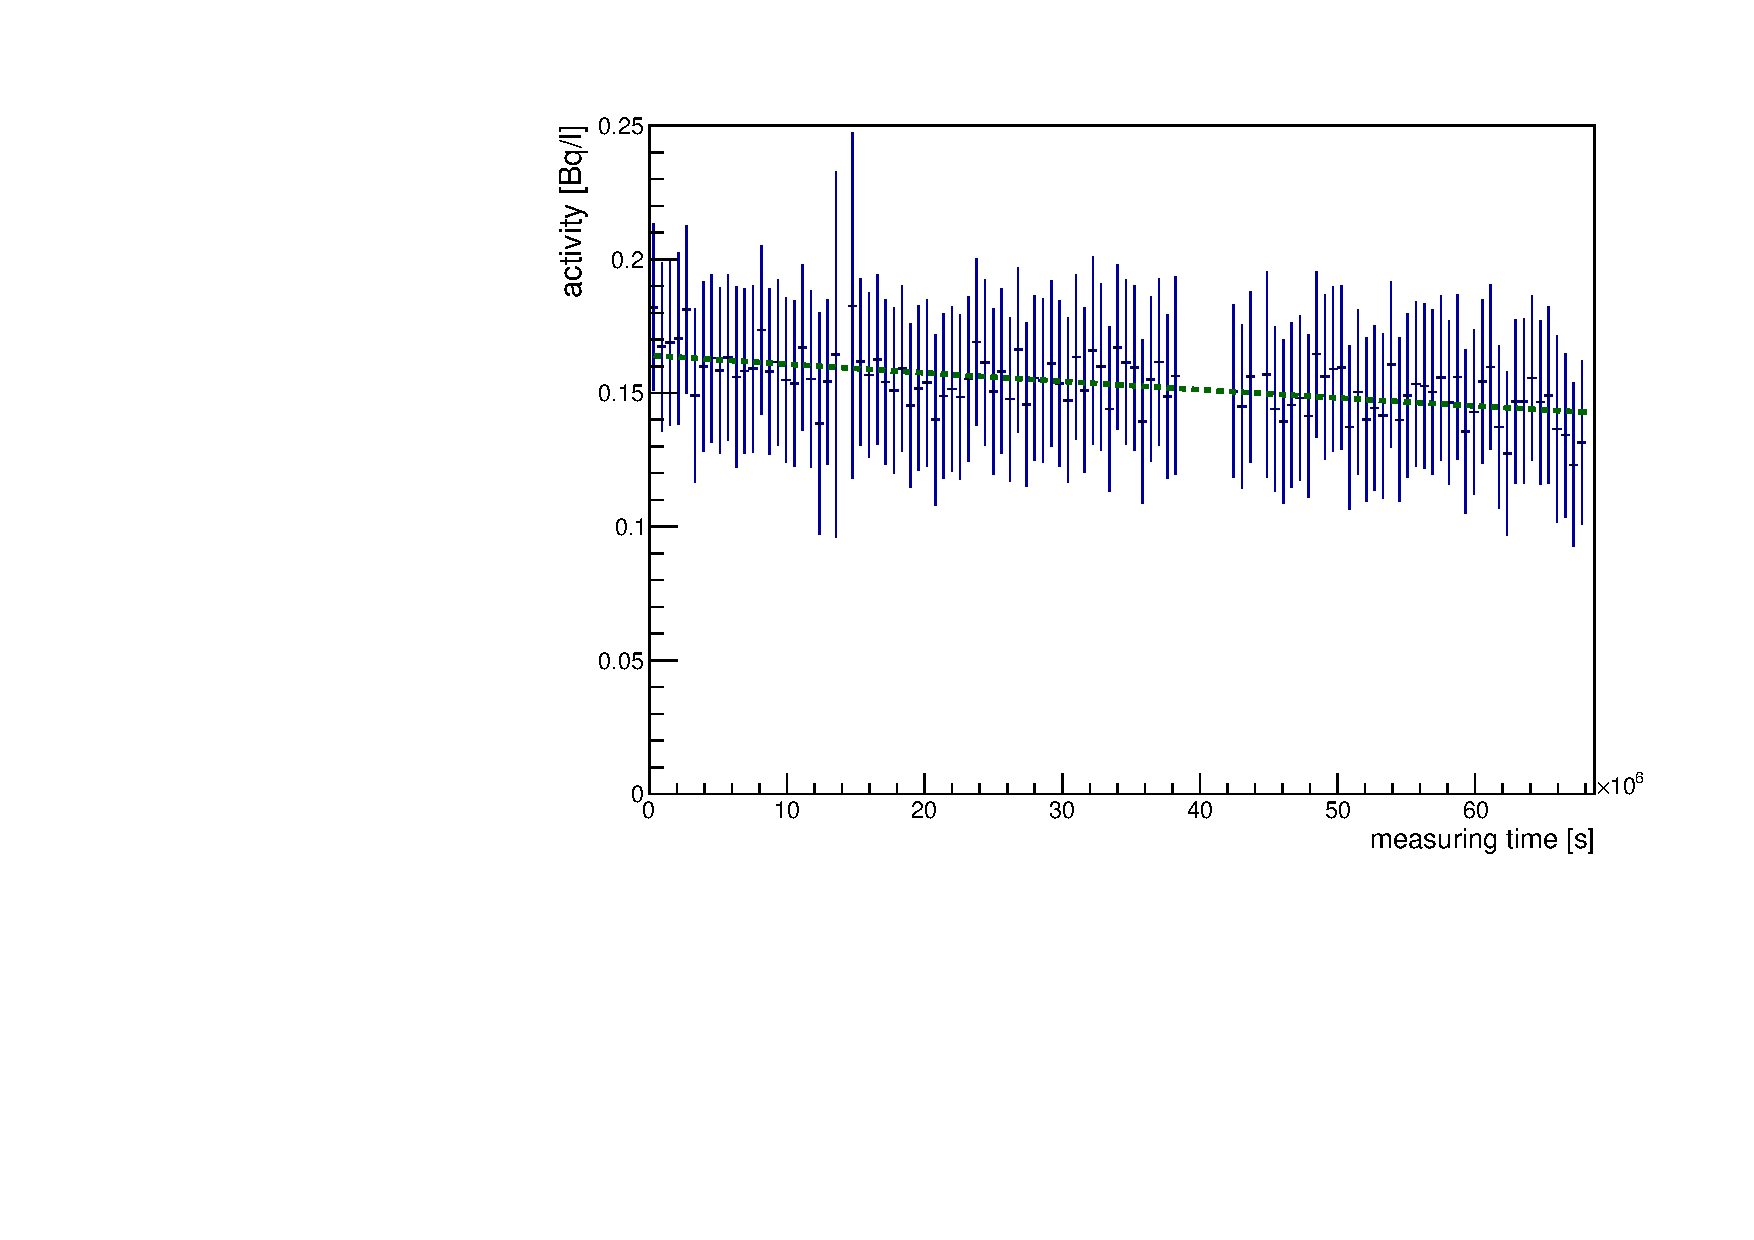
\includegraphics[width=\textwidth]{./Bilder/Aktivitaet.pdf}
		\caption{specific activity of \Kr over time}
		\label{fig:activity}
	\end{minipage}
\end{figure}
\section{Monte Carlo simulation}
\label{sec:MonteCarlo2}


!!!!! zur deadlayer noch genauer was heraussuchen !!!!!

To calculate this conversion factor we have to apply the same process as in the line count rate analysis.
Just that we this time don't simulate the emission of photons with an energy of 514keV in the liquid argon but rather simulate the actual \Kr decays themselves.
But a problem is, that we can expect the detector efficiency of \Kr to be very small.#
This is because the electrons probability of being detected is being suppressed by the fact the detectors themselves have a small dead layer of germanium around them.
If an electron is captured in this dead layer it will create no signal that could be recored even though it hit the detector.
On the other hand if a photon hits the detector it is very likely to deposit all of its energy inside the active detector area due to it being able to transmit further into the detector.
It also has to be considered that only those decays will be considered by us that made their event in one of the detectors that was always on.
Every other decay that made an event in another detector will be discarded making the detector efficiency even smaller. 
Because of this low expected detector efficiency we have to simulate a much higher amount of decays than photons were emitted in the other simulation.
\\

In this simulation we simulated N = 1 billion \Kr decays in a volume of again $V_{sim} = 17.65 \mathrm{m}^3$.
Due to the massive amount of simulated events only those decays were saved in which an event has been measured.
These events created a combined spectrum of the emitted electrons plus the photons emitted from the excited \nuc{Rb}{85m} as seen in figure \ref{fig:Sim1Spektrum}.
If you compare this spectrum with the one calculated for the other Monte Carlo simulation we can see these two spectra look very much alike.
But this would mean that the majority of the measured events must have been caused by the photons of the \nuc{Rb}{85m} relaxation.
That would also mean that almost none of the electrons emitted in the beta decay of \Kr created any signal.
This is actually an advantage for us.
If the majority of the measured events were created by electrons then we would have to apply a correction onto our detector efficiency.
This is because of a weakness of the simulated detectors.
The dead layer of the actual detectors isn't known that well which is why the simulated detectors can only work with an assumptions of the actual dead volume of the detectors.
Unfortunately, it's hard to correct the determined value for this weakness.
We are therefor in luck that the 514keV photons are responsible for the majority of event in the spectrum.
In this case no such correction has to be applied.
\\

But this conclusion of photons being the main cause of the spectrum assumes that in both simulations the same environmental conditions were simulated.
Whether this is true or not can easily be determined by looking at line count of the characteristic 514keV peak.
In the case of the first simulation an amount of 10179 events were measured by the BEGe detectors in the 514keV peak with a decay density of about 2832 $\unit{photon}/\unit{l}$.
On the other hand in the second simulation only 817 events were measured with a decay density of 56640$\unit{decay}/\unit{l}$.
But one has to consider that in the case of the first simulation only the photons of the \nuc{Rb}{85m} relaxation were emitted and \Kr only decays into this exited state with a probability of 0.434$\%$.
The effective decay density of the first simulation is therefor about 652511 $\unit{decay}/\unit{l}$.
To compare these two line counts, we now have to scale one of the two values so that they would theoretically have had the same decay density.
By applying the scale of $\frac{56640}{652511}$ onto the amount of events in the 514keV peak from the first simulation you get a adjusted value of 884 events.
The fact, that this value is roughly the same size as the value 817 form the second simulation, proves, that a similar environmental situation must have been simulated.
This conclusion also justifies retroactively the simplification in the first simulation of only emitting photons to replace the actual decay could be done.
\\

Now to calculating the conversation factor from this simulation.
Like we need the amount of events measured in the range of interest.
In this case we determine an amount of $\Delta$N = (1438$\pm$38) events in the spectrum that deposited an energy between 200 to 400keV.
With the absolute amount N of decays simulated we determine a detector efficiency of
\begin{equation*}
    \epsilon_{\beta} = \frac{\Delta \mathrm{N}}{\mathrm{N}} = (1.438\pm0.038)\times10^{-6} \frac{\unit{events}}{\unit{decay}}
\end{equation*}
This values says that any decay in the liquid argon has a probability of $\epsilon_{\beta}$ to be detected by one of the detectors that was always on.
With this value we can again calculate the volume independent conversation factor
\begin{equation*}
    \frac{1}{\epsilon_{\beta} V_{sim}} = (39.38\pm1.04) \frac{\unit{decay}}{\unit{events} \times l }
\end{equation*}
\\

With this conversation factor we can now also calculate the specific activity of \Kr.
By applying equation \ref{equ:activityAt0} and feeding it with the values found we result in an specific activity of $a = (0.0614\pm0.0419) \frac{\unit{Bq}}{\unit{l}}$ at the start of Phase II.

\begin{equation}
    a(t=0) = \frac{R_\mathrm{count}}{\epsilon_{\beta} V_{sim}} 
    \label{equ:activityAt0}
\end{equation}

We can get back to the graph \ref{fig:ChangeInEventRateFit} and apply the same formula to each of its values and the fit function.
The resulting graph can be seen in figure \ref
Because we want to compare this value to the specific activity found in the line count rate analysis, we have to now calculate the mean specific activity over all of Phase II.
This can easily be done by integrating an exponential decay function over all of \PII~ and then dividing it by 2.17 years.

\begin{equation*}
    \bar{a} = \frac{1}{2.17\unit{y}} \int_0^{2.17y} a(t=0)\times\exp \left( \frac{\log(2)}{T} t \right) \mathrm{d}t
\end{equation*}
with T being the half life of \Kr.
This results in an mean specific activity of $ \bar{a_{2}} = 57.294 \frac{\unit{mBq}}{\unit{l}}$.
\\

If you now compared this result with the specific activity found in the line count rate analysis you will realize that there is a problem.
The mean specific activity of all investigated detectors found in the first method had a value of $\bar{a}_{1} = (5.08\pm0.857)\times10^{-4}\frac{\unit{Bq}}{\unit{l}}$.
Compared to this is the value determined here two orders of magnitude bigger.
This is problematic.
But in actuality we could have seen this problem coming.
Because if we would expect the amplitude of the function shown in figure \ref{fig:activity} to be in the same order of magnitude as the other activity we determined, no real change should be seen over the uncertainty.
The critical question are now: 
Which of the methods is faulty, which of the assumption we used was wrong and can we still make a statement about \Kr specific activity from the problematic approach.
These question will be answers in the following section.
\\


\section{Discussion}
\label{Discussion}

The biggest advantage of the line count rate analysis compared to the second method is that in its case the investigated effect can only originate from \Kr and no other isotope.
Because of this the likelihood of its determined value being the actual specific activity is relatively high.
By comparing the results of the first method with those of the WARP and Darkside experiments, we have already seen that the specific activity of \Kr is lower than in all other experiments.
The second method however has the problem that theoretically every other isotope that is residual in the liquid argon contributes to the investigated change over time.
It can therefor be very likely that our mistakes lies in the assumption that all contribution of any other isotope to this change can be ignored. 
In the beginning of this chapter we already discussed all of the isotopes that are the most probable sources of error.
We already mentioned there that any contributions from \nuc{Ar}{39} and \nuc{Po}{210} can be disregarded due to their either high half life or their high mean kinetic energy of the escaping particle.
But as it was already indicated there, it might be necessary to discuss the influence of \nuc{Ar}{42} further.
\nuc{Ar}{42} has a half life of 32.9 y which is in the same order of magnitude as the half life of \Kr.
Therefore, we can expect to see a change in its activity over the course of \PII~ of about 4.4$\%$ of its absolute specific activity.
With an specific activity big enough one could expect this isotope to be responsible for the measured decrease.
But due to the fact that \nuc{Ar}{42}'s specific activity has already been determined to be much lower than the measured amplitude it can not be the only cause of this .
\\

But what is really interesting about \nuc{Ar}{42}, is not the decay of \nuc{Ar}{42} itself, but rather the contributions of the daughter nuclei \nuc{K}{42}.
\nuc{K}{42} has a half life of 12.355 h \cite{chen_nuclear_2016}.
It can now be approximated, that \nuc{K}{42}'s specific activity is equal to \nuc{Ar}{42}'s specific activity.
This can be assumed, because in comparison to the half life of \nuc{Ar}{42} the resulting \nuc{K}{42} practically decays instantaneously.
This means that it is possible to directly assign one \nuc{K}{42} decay to each \nuc{Ar}{42} that decays.
This doubles the number of decays which can be attributed to \nuc{Ar}{42}.
But assuming that the individual \nuc{Ar}{42} and \nuc{K}{42} isotopes are homogeneously distributed in the liquid argon, their combined specific activity is still by far not big enough to explain the bigger amplitude measured.
\\

And here comes the critical point.
The \nuc{K}{42} isotopes are not homogeneously distributed in the liquid argon.
To understand why they are not we have look at what a \nuc{K}{42} does right after it is formed.
Right after a \nuc{Ar}{42} decays is the resulting \nuc{K}{42} isotope positively ionized.
This results from the newly formed electron escaping from the decay position due to its high velocity.
Because the \nuc{K}{42} isotope is positively charged, it is its aim to reduce its potential energy created by electrostatic fields.
\\

Such fields are present in the liquid argon tank originate from the germanium detectors.
In a germanium detector it is necessary to create a great electrostatic potential difference between the doped electrodes.
The resulting electric field separates electron-hole pairs that might have been created by other particles depositing their energy in the semiconductor \cite{spieler_semiconductor_2005}.
The field then guids the particles to the respective electrodes and by that creating a current which can be measured externally.
In the case of the GERDA experiment are strong fields necessary.
They are supposed to guarantee that the majority of electron-hole pairs reach the corresponding electrodes much faster than their mean free time $\tau$. %Hier noch die Buchquelle
If the fields would not be as strong, the detection probability of any event would be much lower which is not ideal for an experiment in which extremely rare events have to be measured.
\\

Now that the positively ionized isotopes see these electrostatic fields of the detectors, they want to move in the direction of the negative charge located on the outer negatively doped surface of the detectors.
Because in the liquid argon the mean time it takes the ionized \nuc{K}{42} to capture an electron as compensate for its positive charge is relatively long. %!!!!! hier brauche ich noch das paper zur charakteritsichen Zeit in der das Nuklid ionisiert ist !!!!!
Thats why even though the fields are not very strong outside of the detectors the \nuc{K}{42} can still travel a relatively long distance before it either captures an electron or decays further. 
However, due to the higher density of \nuc{K}{42} isotopes near the germanium detectors it can be expected that also the specific activity around the detector increases.
\\

This effect has already been measured in the GERDA set up and it is one of the greatest background sources of the whole experiment.
\nuc{K}{42} has also the unfortunate characteristic for the GERDA experiment that its Q-value at about $Q_{\beta}=3525\unit{MeV}$ lies higher than the Q-value of the double beta decay of \nuc{Ge}{76} $Q_{\beta \beta} = 2039\unit{MeV}$.
This means that electrons of the \nuc{K}{42} decay can create background events in the investigated rage. 
Initially it was not expected to create much background.
Its influence on the measurement however was only recognized after the start of \PI, when its counting rate was too high by a factor of 20. \cite{becerici_schmidt_results_2014}. %!!!!! Refernz zu Becerici Schmidt 
Techniques to suppress the background of \nuc{K}{42} were introduced over time like the usage of nylon mini-shrouds as a mechanically barrier.
The mini-shrouds together with active filters of the pulse shape analysis and the liquid argon veto have proven to bee able to suppress \nuc{K}{42} events by more then three orders of magnitude.
\\

In this case however it is not possible for the analysis to use the active filters to suppress the \nuc{K}{42} further.
Because otherwise we would also filter out the \Kr events that we wanted to investigate in the first place.
So it still can be expected that a not negligible proportion of the measured specific activity comes from the denser \nuc{K}{42} in the region of the detectors.
What effective specific activity can be expected from the \nuc{Ar}{42} is difficult to estimate, but you can assume that it should be far greater than that of \Kr.
To get a quantitative approximation, you can now use the plot of the event rate change again (see \ref{fig:ChangeInEventRate}) and modify the fit function used so that two exponential decays plus a constant background are taken into account.
Both of the exponential decay fit functions have their half life fixed to the respective values of \Kr (10.739y) and \nuc{Ar}{42} (32.9y).
The used fit function can be seen in equation \ref{fig:double}, the resulting fit function in figure and the fit parameter in table.
\begin{equation}
    \mathrm{f}(x) = \mathrm{A}\times\exp\left(-\frac{\log(2)}{\mathrm{B}} x \right) + \mathrm{C}\times\exp\left(-\frac{\log(2)}{\mathrm{D}} x \right) + \mathrm{E}
\end{equation}

\begin{figure}[t!]
	\centering
	\begin{minipage}{.5\textwidth}
	\centering
	\ifmakefigures%
	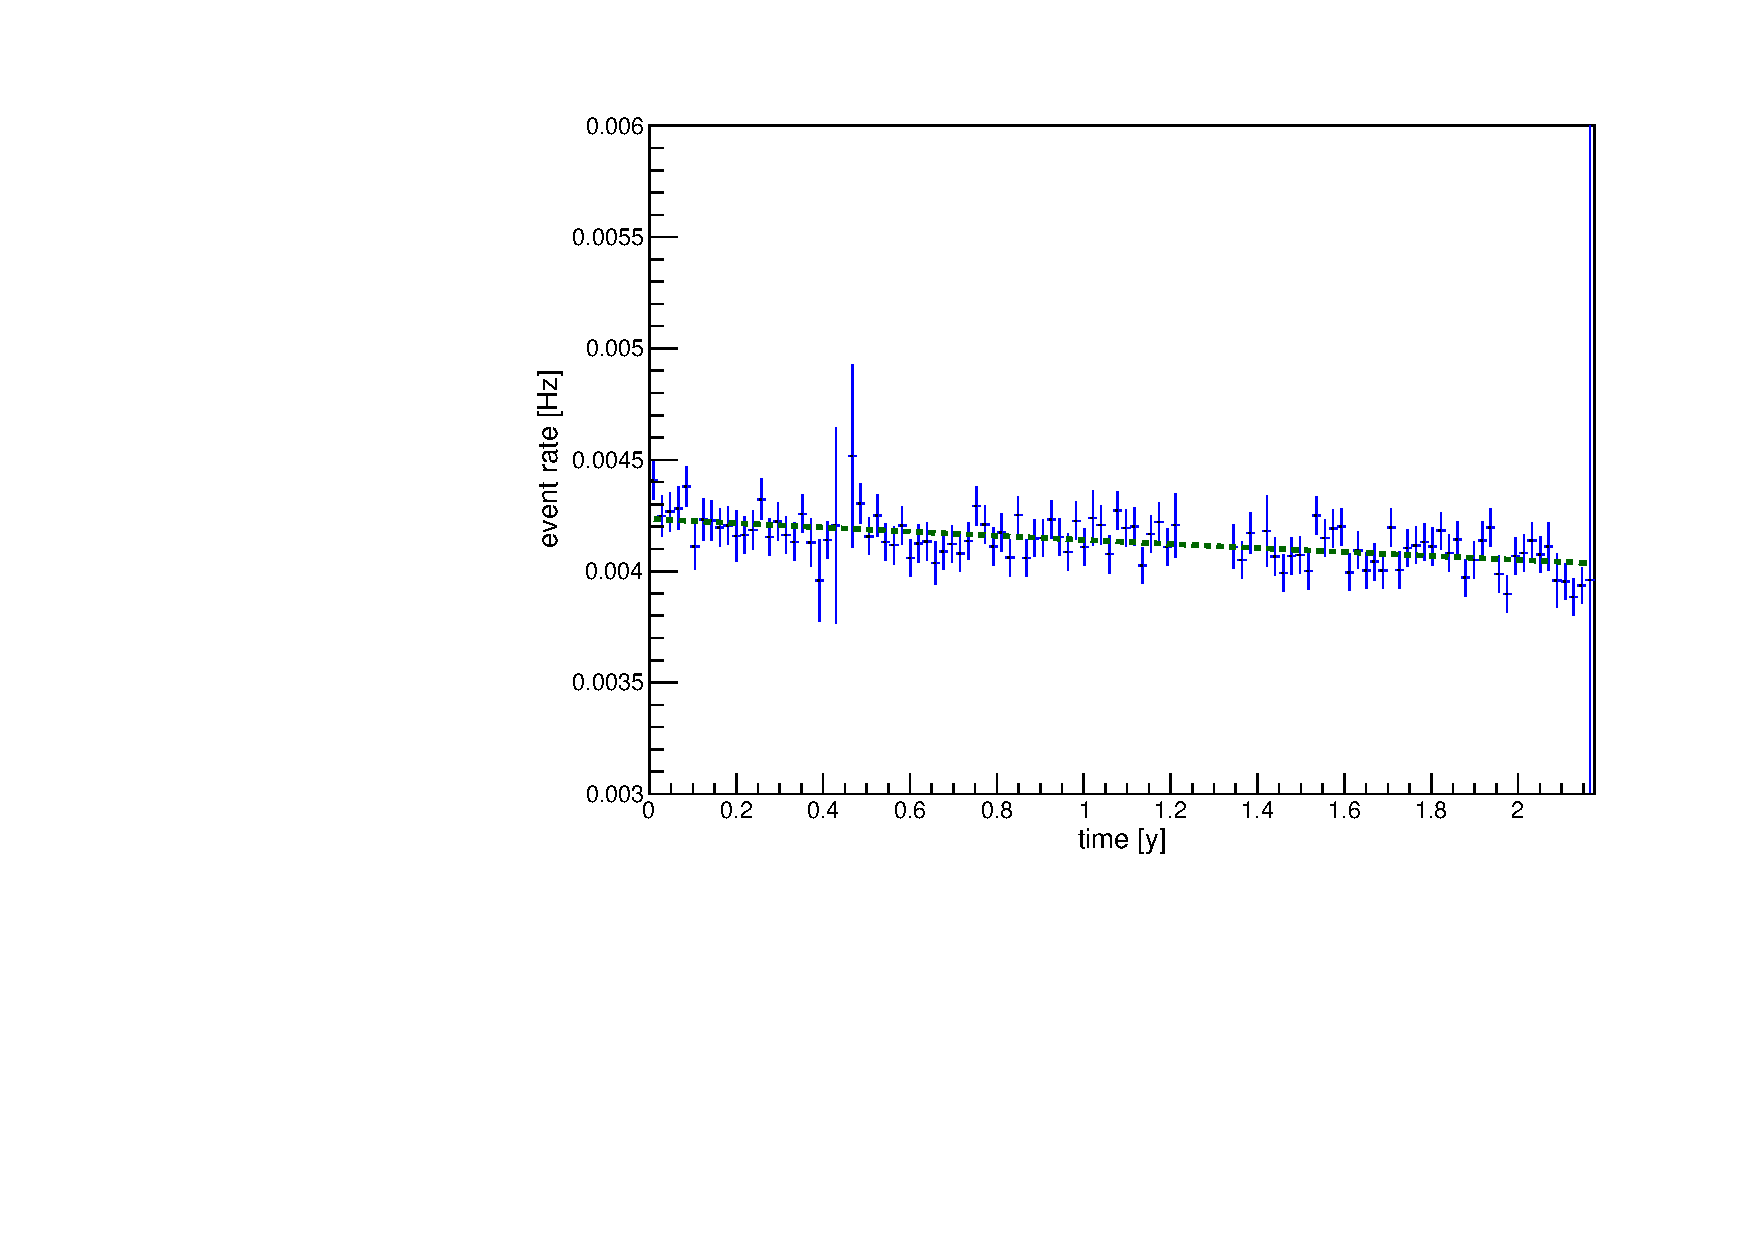
\includegraphics[width=75mm]{./Bilder/doppelt.pdf}
	\fi%
	\caption{double exponential decay fit}
	\label{fig:double}
	\end{minipage}%
	\begin{minipage}{.5\textwidth}
    \centering
    \begin{tabular}{|l|c|}
        \hline
        Name  & Value \\
        \hline
        A     & 0.0010244$\pm$0.000122073 \\
        \hline
        B    & 10.739 \\
        \hline
        C   & 0.00145395$\pm$0.000129916 \\
        \hline
        D  & 32.9 \\
        \hline
        E & 0.00175652$\pm$0.000119112 \\
        \hline
    \end{tabular}
    \captionof{table}{}{Fit parameters of the double exponential decay analysis}
    \label{tab:doubleFitpara}
	\end{minipage}
\end{figure}


In a direct comparison of figure \ref{fig:double} with graph \ref{fig:ChangeInEventRateFit} no real difference can be see.
But when looking at the fit parameters you can see that in this case the \nuc{Ar}{42} exponential fit function has a bigger amplitude than \Kr.
Because the \nuc{K}{42} density is not homogeneously distributed in the liquid argon it is impossible to run a Monte Carlo simulation to again determine a new detector efficiency.
But using the conversation factor determined from the second simulation to make an estimate the respective effective specific activities can be calculated to $(40.4\pm0.59)\frac{\unit{mBq}}{\unit{l}}$ for \Kr and $(57.3\pm0.66)\frac{\unit{mBq}}{\unit{l}}$ for all of the decays resulting from \nuc{Ar}{42}.
These values are both still way to high for what was expected from them.
For the \Kr it is obvious but for \nuc{Ar}{42} the maximum effective specific activity expected to be measured should have only been about one orders of magnitude higher than the actual specific activity of only the \nuc{Ar}{42}.
Due to the fit parameters still generating far too much specific activity for these isotopes shows that other sources of change are still not accounted for.
Nevertheless it has been shown with this fit that \Kr does not contribute solemnly to the change of count rate over time and with this the assumption from before has been shown to be false.
\\

Theoretically it would now still be possible to determine an specific activity of \Kr from plot \ref{fig:ChangeInEventRate} but considerein every individual source of change in count rate.
But because of the higher number of fit parameters that would have to be determined and the relatively large uncertainties in the plot compared to the overall change, it is not difficult to be pessimistic whether this analysis can even make a statement about the specific activity of \Kr.
\\

At the end of this analysis it is again of interest to investigate how the change in the count rate would have looked over time if the specific activities of the WARP or the Darkside experiment had been present.
Again, in the case of the WARP experiment an activity of $(0.16\pm0.13)\frac{\unit{Bq}}{\unit{l}}$ was measured. 
If one would plot its equivalent amplitude in a diagram like Figure \ref{fig:ChangeInEventRateFit} a significant change would have been visible.
On the other hand is the activity in the Darkside experiment with its $(2.8577 \pm 0.18122) \frac{\unit{mBq}}{\unit{l}}$ too small to measure an apparent change over time.
\\

% use fit to calculate the decrease in rate of the signals in range from 200 to 500keV
% from fit and assumption that only Kr85's activity is decreasing one can calculate the specific activity from the amplitude of the fit

% use Volume of LAr-Tank to determine the number of Kr85 and from this the concentration in the argon

\chapter{Summary and Outlook}
\label{sec:ConcAndOutlook}

With the line count rate analysis carried out in this paper it could be shown that the specific activity of \nuc{Kr}{85} in the liquid argon of the GERDA experiment has a value of $(0.508\pm0.0857) \frac{\unit{mBq}}{\unit{l}}$. 
Compared to WARPs $(160\pm130)\frac{\unit{mBq}}{\unit{l}}$ and to Darksides $(2.8577 \pm 0.18122) \frac{\unit{mBq}}{\unit{l}}$ its value is much smaller.
On the other hand, the second attempt to determine a value for the specific activity via the change of count rate over time has failed.
This was due to the falsely made assumption that \Kr is the only isotope in the liquid argon to show significant change in its activity over time.
\\




%%%%%%%%%%%%%%%%%%%%%%%%%%%%%%%%%%%%%%%%%%%%%%%%%%%%%%%%%%%%%%%%%%%%%%%%%%%%%%%%
% -----------------------------------------------  ADD SOME ACKNOWLEDGMENTS  ---
%%%%%%%%%%%%%%%%%%%%%%%%%%%%%%%%%%%%%%%%%%%%%%%%%%%%%%%%%%%%%%%%%%%%%%%%%%%%%%%%
\section*{Acknowledgments}

%%%%%%%%%%%%%%%%%%%%%%%%%%%%%%%%%%%%%%%%%%%%%%%%%%%%%%%%%%%%%%%%%%%%%%%%%%%%%%%%
%%%%%%%%%%%%%%%%%%%%%%%%%%%%%%%%%%%%%%%%%%%%%%%%%%%%%%%%%%%%%%%%%%%%%%%%%%%%%%%%

%----------------------------------------------------------------- appendix ----
%%%%%%%%%%%%%%%%%%%%%%%%%%%%%%%%%%%%%%%%%%%%%%%%%%%%%%%%%%%%%%%%%%%%%%%%%%%%%%%%
% --------------------------------------------------- ADD APPENDIX (IN CASE) ---
%%%%%%%%%%%%%%%%%%%%%%%%%%%%%%%%%%%%%%%%%%%%%%%%%%%%%%%%%%%%%%%%%%%%%%%%%%%%%%%%
\appendix

\section{Determining the resolution of the detector types}
\label{sec:ResDetermination}
rgdagadgadgdsgdsgrsgserg



% \section{}
% \label{}

%--------------------------------------------------------------- references ----
\backmatter

\bibliographystyle{plain}
\bibliography{references}
\listoffigures
\listoftables

\end{document}
